\documentclass[10pt,a4paper]{article}
\usepackage[margin=2.3cm,headheight=14pt]{geometry}
\usepackage{fontspec,unicode-math}
\setmainfont{Libertinus Serif}
\setsansfont{IBM Plex Sans}
\setmonofont[Scale=0.86]{IBM Plex Mono}
\setmathfont{Libertinus Math}
\usepackage{microtype,graphicx,booktabs,tabularx,xltabular,xcolor,float,fvextra,caption,fancyhdr,titlesec,enumitem,multicol,array}
\usepackage{placeins}
\usepackage[numbers,sort&compress]{natbib}
\usepackage[colorlinks,hypertexnames=false,linkcolor=teal!70!black,citecolor=teal!70!black,urlcolor=teal!70!black]{hyperref}
\newfloat{listing}{tbp}{lol}\floatname{listing}{Listing}
\captionsetup{font=small,labelfont=bf}
\renewcommand{\tabularxcolumn}[1]{>{\raggedright\arraybackslash}p{#1}}
\setlength{\tabcolsep}{4pt}
\setlength{\LTpre}{6pt}\setlength{\LTpost}{6pt}
\setlength{\emergencystretch}{3em}
\setlist{itemsep=2pt,topsep=4pt}
\newcommand{\ax}[1]{\par{\raggedright\noindent\hangindent=2.2em\hangafter=1 $#1$\par}\smallskip}
\titleformat{\section}{\sffamily\Large\bfseries\color{teal!55!black}}{\thesection}{0.8em}{}
\titleformat{\subsection}{\sffamily\large\bfseries}{\thesubsection}{0.7em}{}
\titleformat{\subsubsection}{\sffamily\normalsize\bfseries}{\thesubsubsection}{0.6em}{}
\renewcommand{\floatpagefraction}{0.75}\renewcommand{\topfraction}{0.85}\renewcommand{\textfraction}{0.12}
\pagestyle{fancy}\fancyhf{}
\fancyhead[L]{\sffamily\footnotesize Representing biomedical experiments: technical report}
\fancyhead[R]{\sffamily\footnotesize\nouppercase{\leftmark}}
\fancyfoot[C]{\sffamily\footnotesize\thepage}
\renewcommand{\headrulewidth}{0.3pt}
\begin{document}
\begin{titlepage}
\sffamily
\vspace*{2.2cm}
\noindent{\color{teal!55!black}\rule{\linewidth}{1.2pt}}\par\vspace{0.6cm}
\noindent{\Huge\bfseries Representing Biomedical Experiments\par}\vspace{0.4cm}
{\Large A conceptual framework, its partonomy\\[2pt] and its description-logic axiomatization\par}\vspace{0.3cm}
{\large with the challenge--rescue experiment as a case study\par}\vspace{0.6cm}
\noindent{\color{teal!55!black}\rule{\linewidth}{1.2pt}}\par\vspace{1.0cm}
{\large Technical report on the experiment layer of the robot science assistant\\ on Cell 01 of the LabAutomationTwin\par}
\vspace{1.4cm}
{\normalsize [Authors and affiliations]\par}
\vfill
{\small\rmfamily
\begin{tabular}{@{}ll@{}}
Generated & 2026-10-17, from the generators' outputs \\
Case study & challenge--rescue experiment, design \texttt{c\_\allowbreak{}d85\_\allowbreak{}t48\_\allowbreak{}n1} \\
Ontology & 174 concepts, 52 object and 12 data properties, 246 TBox axioms (OWL~2~DL), HermiT-checked \\
Status & research prototype; biology is a surrogate, quantities ILLUSTRATIVE (D016) \\
\end{tabular}\par}
\end{titlepage}
\pagenumbering{roman}
\tableofcontents
\clearpage
\pagenumbering{arabic}

\section{Executive summary}\label{sec:summary}
A robot scientist has to do more with an experiment than execute it. It has to know why each step is there, which
culture plays which part, what a measurement stands for, which comparison answers which question, and whether the
design can support the conclusion it is meant to support---ideally before anything is pipetted. This report describes
how the experiment layer of the robot science assistant (RSA) on Cell~01 of the LabAutomationTwin came to represent
experiments in that way, and what the resulting representation can and cannot check.

\paragraph{The case.} The running example is a \emph{challenge--rescue} experiment on organoid cultures
(Section~\ref{sec:case}): two cultures are injured with a challenge agent, one of them is given a rescue agent
48~h later, an untreated culture serves as control, and organoid size is imaged at 72~h. The experiment
discriminates three recovery hypotheses---graded recovery, a threshold (``point of no return''), and a protective
response that moves the threshold. The design \texttt{c\_\allowbreak{}d85\_\allowbreak{}t48\_\allowbreak{}n1} was selected for its expected information gain of
0.5439~bit over the hypotheses. All biology is Cell~01's illustrative surrogate (D016).

\paragraph{From action lists to experiment logic.} The representation was developed in nine steps
(Section~\ref{sec:evolution}): from a culture-level plan of 12 actions ordered by causal links, through
CRAM/RPL plans and entity designators, to the observation that the experiment's \emph{logic} is three cultures,
each defined by its treatment, compared pairwise so that each comparison isolates one exposure. Written that way
(\texttt{experiment.ldl}), the experiment is short, has no variables, and the 13 culture actions and their
order are \emph{derived} from it; the derivation reproduces all 12 actions of the hand-written plan and adds
the validity analysis that the hand-written plan only implied.

\paragraph{A conceptual framework.} Generalising from the case, Section~\ref{sec:framework} proposes a framework of
five layers---epistemic, design, protocol, execution and biological system---that keeps apart what is
\emph{planned}, what \emph{happens}, what is \emph{measured} and what is \emph{believed}. Its core concepts (units,
factors and levels, arms, controls defined by what they control for, replicates, readouts as proxies, comparisons,
interaction contrasts, analysis plans, hypotheses that \emph{posit} biology, belief and information gain,
deviations, conclusions) organise a multi-axial taxonomy of experiments. Validity criteria are assigned to the
mechanism that can enforce them: description logic for what experiments \emph{are}, closed-world queries for what a
design \emph{must contain}, run-time monitors for what an execution \emph{must keep}, and probabilistic models for
what it \emph{will tell us}. Three partonomies (process, material, plan) are separated from containment, membership,
participation and realization (Section~\ref{sec:partonomy}).

\paragraph{Axiomatization and reasoning.} The framework is axiomatized in OWL~2~DL (Section~\ref{sec:owl}):
246 TBox axioms over 174 concepts in 13 groups, 71 of them definitions, so that the HermiT
reasoner \emph{classifies} arms, comparisons, designs and experiments from their content. Closure axioms in the ABox
make the definitions with negation decidable. The ontology is consistent alone, with both designs, and together with
Cell~01's biology ontology; all 8 negative controls are detected as inconsistencies; 30 subsumptions
between experiment classes are inferred rather than stated. What OWL~2 cannot express---single-factor contrasts,
replicate counts, plate-edge placement, factorial coverage, interaction estimability---is checked by closed-world
queries (Section~\ref{sec:closed}).

\paragraph{The main finding.} The reasoner classifies the current experiment as a \emph{validated injury--rescue}
experiment that is hypothesis-discriminating, sufficiently informative, pre-specified and well contrasted, but
\emph{not} as adequately controlled: it lacks a rescue-only arm (so the interaction of injury and rescue is not
estimable), a vehicle arm, a positive control and replicates, and its wells lie on the plate edge. An improved,
ILLUSTRATIVE design---a challenge $\times$ time-of-rescue factorial with 5 arms, 15 units and
5 comparisons including a therapeutic-window contrast---is classified as an
\emph{adequately controlled injury--rescue design}, and each variant that removes one ingredient loses exactly the
corresponding class (Section~\ref{sec:results}). The critique a biomedical reviewer would make is thus available as
a formal result before the experiment is run.

\paragraph{What our laboratory affords.} Laboratories are built for classes of experiments, so the ontology also
describes laboratories (Section~\ref{sec:afford}). Capability classes are defined by the functions a laboratory's
devices bear, its environments and its validated readouts; requirement classes are defined by a design's content.
HermiT classifies Cell~01, from its 10 component records, as a treatment-and-imaging module that is dosing,
cultivation, imaging, quality-controlled, containment-capable and connected, but not an endpoint-reader or
multi-environment laboratory. Matched against it, the current design is executable in Cell~01; the improved design
lacks only a vehicle stock and, with it, needs two dosing sessions per time point (at most 11 wells fit an
excursion); an ATP endpoint is executable on site with a transfer to an ILLUSTRATIVE core plate reader; and a design
with an oxygen factor is not executable, because no laboratory provides two environments.

\paragraph{Limits.} The CRAM plans are not executed (no Lisp CRAM is installed); the factors and analysis plan exist
in the OWL layer but not yet in the authored LDL; BFO and OBI are followed in style, not imported; the replication
minimum and the information target are illustrative criteria; in vivo and clinical experiments are outside the
current taxonomy (Section~\ref{sec:limits}).


\section{Motivation and scope}\label{sec:motivation}
Laboratory automation has made it routine for robots to \emph{perform} protocols. Robot scientists such as Adam and
Eve \citep{king2009,williams2015} went further and closed the loop from hypothesis to experiment to analysis, and
self-driving laboratories in chemistry and materials science \citep{burger2020,abolhasani2023} have shown how far
closed-loop experimentation can go when the experiment space is well parameterised. Biomedical experiments are
harder to parameterise: the system is alive, the quantities of interest are hidden and reached only through proxies,
and whether an experiment supports its conclusion depends on its \emph{logic}---which cultures are compared, what
they differ in, which controls exclude which alternative explanation---more than on any single step. Poor design is
one of the recognised causes of irreproducible biomedical results \citep{baker2016}, and reporting guidelines such
as ARRIVE \citep{kilkenny2010} and CONSORT \citep{schulz2010} exist largely to make that logic explicit after the
fact.

For a robot scientist the logic has to be explicit \emph{before} the fact, in a form a program can inspect. The RSA
already derives culture-level plans, refines them into lab actions and motions, and audits their execution (see the
companion report on the RSA kernel). What it lacked was a representation of the experiment \emph{as an experiment}:
of its question and hypotheses, its units and their roles, its treatments, its comparisons and their purpose, and
the standards against which a design is judged. This report fills that gap. Its contributions are:
\begin{enumerate}
\item a sequence of representations of one experiment, from an ordered list of actions to a variable-free entity
  designator organised by the experiment's logic, with the actions and their order derived and checked
  (Sections~\ref{sec:case}--\ref{sec:authored});
\item a conceptual framework for biomedical experiments in five layers, with core concepts, a multi-axial taxonomy,
  validity criteria assigned to enforcement mechanisms, and a lifecycle (Section~\ref{sec:framework});
\item a partonomy that separates process, material and plan parthood from containment, membership, participation and
  realization (Section~\ref{sec:partonomy});
\item two formalisations: an LDL concept hierarchy with a closed-world checker (Section~\ref{sec:ldlconcepts}) and an
  OWL~2~DL axiomatization with defined concepts, classified and checked by HermiT (Sections~\ref{sec:dlv1}--\ref{sec:results});
\item an evaluation on the case study and on an improved design, with negative controls at every level.
\end{enumerate}
The scope is the in-vitro injury--rescue family of experiments; the framework is written to extend beyond it, and
Section~\ref{sec:limits} lists what that extension still requires.


\section{Background}\label{sec:background}
\subsection{Experimental design}
The vocabulary of controlled experimentation goes back to Fisher \citep{fisher1935}: experimental units, treatments,
replication to estimate chance variation, randomisation to protect against systematic bias, and blocking to remove
known sources of variation. For laboratory biology, Lazic \citep{lazic2016} gives a modern account; it stresses that
the experimental unit is the entity \emph{independently} assigned to a treatment (a culture, not a measurement of it),
that technical and biological replicates answer different questions, and that controls are defined by what they rule
out. Factorial designs vary several factors at once and make their interactions estimable. Clinical trials use the
same notions under other names: arms, epochs and the cells of an arm-by-epoch grid, as formalised in the CDISC Study
Design Model \citep{cdisc_sdm}.

\subsection{Ontologies of experiments}
Ontologies of scientific experiments were proposed early: EXPO \citep{soldatova2006} describes experiments as
investigations with hypotheses, designs, objects and results; EXACT \citep{soldatova2008} describes protocols as
sequences of actions. The Ontology for Biomedical Investigations (OBI) \citep{brinkman2010,bandrowski2016}, part of
the OBO Foundry \citep{smith2007}, models investigations as planned processes that realize plans, assays with
specified inputs and outputs, study designs and their independent variables, and roles borne by material entities;
it is built on the Basic Formal Ontology (BFO) \citep{arp2015}, which separates continuants (material entities,
qualities, roles, dispositions) from occurrents (processes). The ISA framework \citep{sansone2012} carries
investigation, study and assay metadata for data deposition. The framework of this report follows BFO and OBI in
style---planned processes execute plans, roles and dispositions are borne, data are about qualities---without
importing them (Section~\ref{sec:limits}).

\subsection{Description logics and OWL}
Description logics \citep{baader2003} are decidable fragments of first-order logic built from concepts and roles.
$\mathcal{SROIQ}(\mathbf{D})$ \citep{horrocks2006} underlies OWL~2~DL \citep{owl2}: it adds role hierarchies,
transitivity, inverse roles, role chains, qualified number restrictions and datatypes. Number restrictions are
allowed only on \emph{simple} roles (roles that are neither transitive nor composite, and have no such sub-roles).
OWL reasons under the open-world assumption: what is not stated is unknown, not false. Checking that a design
\emph{contains} something is therefore a closed-world question, usually answered with constraint languages such as
SHACL \citep{shacl2017} or with integrity-constraint semantics \citep{motik2009}. Concrete domains with feature chains
\citep{baader1991} can compare data values reached by different paths, which OWL~2 cannot. HermiT \citep{glimm2014} is
a hypertableau reasoner for OWL~2; Owlready2 \citep{lamy2017} embeds ontologies and reasoners in Python.

\subsection{Plans and Bayesian design in the RSA}
The RSA represents plans in a lab designator language (LDL) and executes them as structured reactive controllers in
the style of RPL and CRAM \citep{mcdermott1991,beetz2001,beetz2010}; knowledge comes from a KnowRob-style ontology
\citep{tenorth2013}. Designs are chosen by expected information gain \citep{lindley1956,chaloner1995}: the mutual
information between the hypotheses and the outcome of a candidate design, estimated by nested Monte Carlo over Cell~01's
surrogate.


\section{The challenge--rescue experiment}\label{sec:case}
\subsection{System, question and hypotheses}
The units are organoid cultures in wells of a microplate, kept in an incubator under a standard culture environment.
Cell~01's surrogate describes each culture by hidden states---injury, an adaptive protective response, a
glutathione-like protective reserve, and viability---driven by two abstract agents: a \emph{challenge} that raises
injury and consumes the reserve, and a \emph{rescue} that restores the reserve and supports recovery. The structure
resembles classic toxicology paradigms in which an antidote's efficacy depends on how late it is given; the project
names no agent, doses are in arbitrary units (au), and every coefficient is a placeholder (D016). Organoid cultures
\citep{sato2009} are a natural target for such experiments because their morphology can be imaged without
destroying them.

Earlier (simulated) data showed that a rescue at 6~h is effective at every challenge dose tested. The open question is
what happens when the rescue comes much later. Table~\ref{tab:hyp} lists the competing hypotheses and the effect each
predicts for the selected design; the effect is the difference in organoid radius between the rescued and the
challenge-only culture at 72~h.

\begin{table}[tbp]\centering\small
\caption{The three recovery hypotheses and their predicted rescue effects for design \texttt{c\_\allowbreak{}d85\_\allowbreak{}t48\_\allowbreak{}n1} (surrogate, ILLUSTRATIVE).}\label{tab:hyp}
\begin{tabularx}{\linewidth}{@{}p{2.4cm}Xp{2.6cm}@{}}\toprule hypothesis & claim & predicted effect (µm) \\ \midrule
M1 graded & recovery declines smoothly with injury and delay; no point of no return & 8.5 $\pm$ 11.4 \\
M2 threshold & once cumulative injury exceeds a threshold, the culture loses its capacity to recover & 25.0 $\pm$ 6.3 \\
M3 protective & as M2, but the adaptive response raises the threshold & 25.4 $\pm$ 6.5 \\
\bottomrule\end{tabularx}\end{table}


\subsection{The selected design}
The planner scored 45 candidate designs (three challenge doses, five rescue delays, one to three wells per arm) by
expected information gain and selected the cheapest design that reaches the required 0.5~bit
(Figure~\ref{fig:eig}). Expected gain grows with the delay, because the hypotheses agree at short delays (all were
calibrated to the effective 6~h rescue) and diverge only at long ones; at 48~h and the highest dose, one well per arm
already gives 0.5439~bit, and two or three wells give 0.601 and 0.641~bit. The resulting design has three
cultures on plate P17: \emph{rescued} (challenge 0.85~au at 0~h, rescue 0.70~au at 48~h, well A01),
\emph{comparator} (challenge only, A02) and \emph{control} (untreated, A05), all imaged at 72~h.

\begin{figure}[tbp]\centering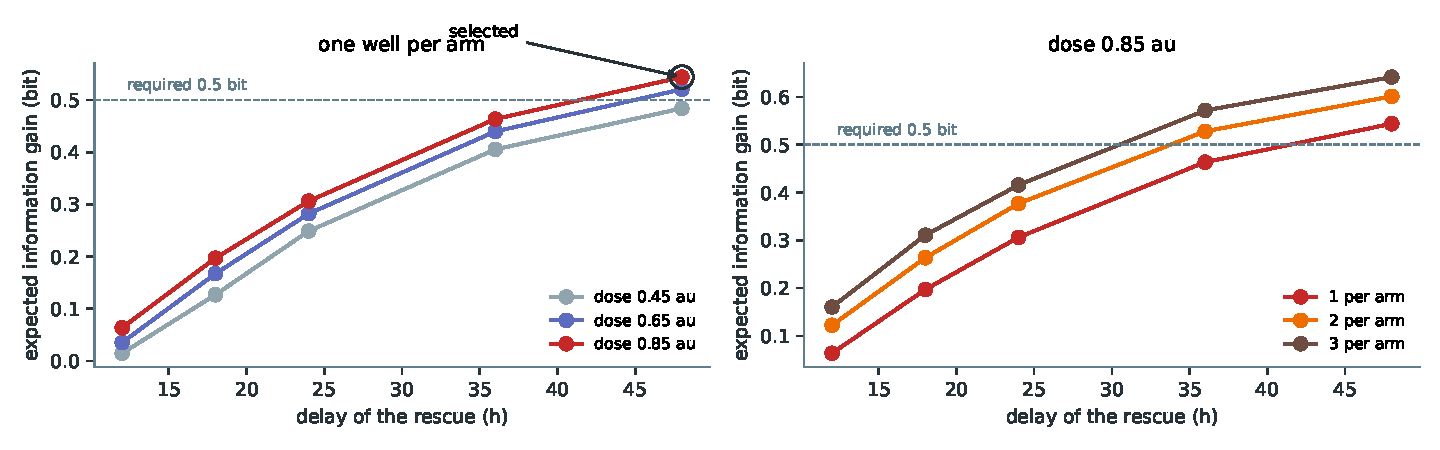
\includegraphics[width=\linewidth,height=0.72\textheight,keepaspectratio]{figures/eig.pdf}
\caption{Expected information gain of the candidate designs over the three hypotheses. Left: one well per arm, by dose and delay; the selected design is circled. Right: the selected dose with one to three wells per arm. Surrogate, ILLUSTRATIVE.}\label{fig:eig}\end{figure}


\subsection{What a run shows}
Executed on the surrogate (Figure~\ref{fig:culture}), the challenge shrinks both challenged cultures; after the
rescue at 48~h the rescued culture partly recovers. At 72~h the radii are 201.6~µm (rescued), 186.8~µm
(comparator) and 267.6~µm (control). The validity comparison shows that the challenge injured the cultures
(-80.8~µm); the primary comparison gives a rescue effect of 14.8~µm. With a measurement noise of
$\sigma \approx$ 2.5~µm, the posterior over the hypotheses moves from uniform to M1 0.68, M2 0.15, M3
0.17: the entropy falls from 1.585 to 1.228~bit, a gain of 0.357~bit in this run against 0.5439~bit expected.
In biological terms: no hard point of no return at 48~h, but a late rescue is clearly weaker than an early one. M2
and M3 predict nearly the same effect in this design; it separates graded from threshold-like recovery, not the two
threshold variants from each other.

\begin{figure}[tbp]\centering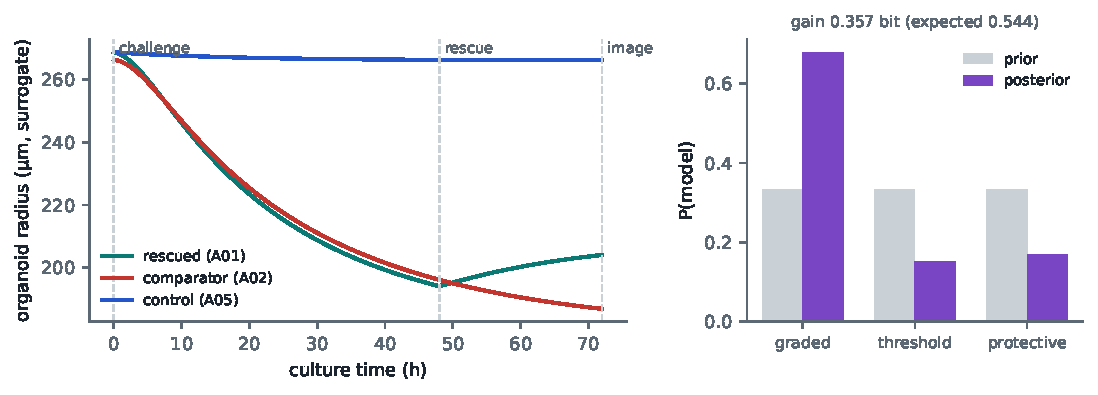
\includegraphics[width=\linewidth,height=0.72\textheight,keepaspectratio]{figures/culture.pdf}
\caption{Surrogate run of the selected design: organoid radius of the three cultures over culture time (left) and the belief over the hypotheses before and after the analysis (right). ILLUSTRATIVE.}\label{fig:culture}\end{figure}


\subsection{How a biomedical reviewer would judge it}
As a real experiment the design would not stand. It has one culture per arm, so culture-to-culture variation cannot be
separated from the treatment effect. It has no rescue-only arm, so part of the rescue effect might be a general growth
effect of the rescue agent rather than rescue of injury. Its control receives nothing while the treated wells receive
liquid, so solvent and volume effects are confounded with the challenge. Its wells lie on the plate's edge row, where
evaporation and temperature effects are strongest. It has a single delay and a single readout, and organoid size is
only a proxy for viability. These are exactly the kinds of defects that a representation of the experiment
\emph{as an experiment} should make visible; Section~\ref{sec:results} shows that the final axiomatization does.


\section{From action lists to experiment logic}\label{sec:evolution}
Table~\ref{tab:evolution} summarises the representations the experiment went through. Each step was prompted by
something the previous one made hard to see; each is generated from the one before it or from its source, and each
was checked mechanically.

\begin{table}[tbp]\centering\footnotesize
\caption{Nine representations of the challenge--rescue experiment.}\label{tab:evolution}
\begin{tabularx}{\linewidth}{@{}p{0.3cm}p{3.0cm}p{3.7cm}XX@{}}\toprule  & representation & file & explicit & derived / checked \\ \midrule
1 & culture-level plan & \texttt{culture\_\allowbreak{}plan.ldl} & 12 actions with physical and knowledge effects & order from causal links (13: 7 physical, 6 knowledge) \\
2 & CRAM/RPL controller & \texttt{culture\_\allowbreak{}plan\_\allowbreak{}src.lisp} & control flow, policies, failure handling & partial order = derived order; refinement into lab designators 8/8 \\
3 & experiment as an entity & \texttt{challenge\_\allowbreak{}rescue\_\allowbreak{}experiment.lisp} & question, materials, rules, steps, insights & one-line top-level plan: \emph{conduct} the experiment \\
4 & nested designators with roles & (superseded) & every participant fills a role; no variables & references identify one step each; after-roles = derived order \\
5 & organised by logic & (superseded) & cultures with treatments, shared conditions, comparisons & single difference per comparison; 12/12 actions regenerated \\
6 & authored experiment designator & \texttt{experiment.ldl} & the logic; validity comparison explicit & 13 actions and order derived; vs.\ the hand-written plan \\
7 & LDL concept hierarchy & \texttt{experiment\_\allowbreak{}concepts.ldl} & 5 experiment concepts, partonomy, procedure & closed-world conformance, classification, 8 negative controls \\
8 & DL statement (v1) & \texttt{experiment\_\allowbreak{}dl.pdf} & the LDL concepts in $\mathcal{SROIQ}(\mathbf{D})$ & simple-role restriction; expressivity of each check \\
9 & OWL~2~DL axiomatization (v2) & \texttt{experiment.ofn} & BFO-style biomedical ontology, defined classes & HermiT consistency, classification, realization; closed-world queries \\
\bottomrule\end{tabularx}\end{table}


\subsection{The culture-level plan}
The first representation states only what is done to the cultures, how they are observed and how the observations
are interpreted and analysed; no plate, instrument or robot appears. Every action states a \emph{physical} effect (on
the cultures' state) and a \emph{knowledge} effect (records, images, estimates, the belief). The order is not written:
it is derived from causal links, a link holding when an effect of one action entails a requirement of another.
Listing~\ref{lst:cp} shows three of the 12 actions; Figure~\ref{fig:poset12} shows the derived order. The plan
is precise, but its logic is implicit: that the comparator exists to isolate the rescue, or that the control licenses
the comparison, can only be reconstructed from requirement lists.

\begin{Verbatim}[fontsize=\scriptsize,breaklines,frame=lines,framesep=2mm]
    (an action ?c1 (type challenging) (culture ?cr) (substance ?ch) (dose 0.85 au) (at (culture-time 0 h))
      (physical (the culture ?cr (exposed-to ?ch 0.85 au)) (the culture ?cr (injury rising)))
      (knowledge (a record (of ?c1) (states ?cr ?ch 0.85 au 0 h))))
    ...
    (an action ?a1 (type analysing) (belief ?B) (statistic (difference (radius ?cr) (radius ?cc)))
      (requires (an estimate (of ?cr) (organoid-radius))
                (an estimate (of ?cc) (organoid-radius))
                (an estimate (of ?ck) (organoid-radius)))                 ; the control licenses the comparison
      (knowledge (the belief ?B (posterior updated)) (the belief ?B (information-gain measured))))))
\end{Verbatim}
\vspace{-4pt}\captionof{listing}{Two of the twelve actions of the culture-level plan (\texttt{culture\_\allowbreak{}plan.ldl}).}\label{lst:cp}\medskip

\begin{figure}[tbp]\centering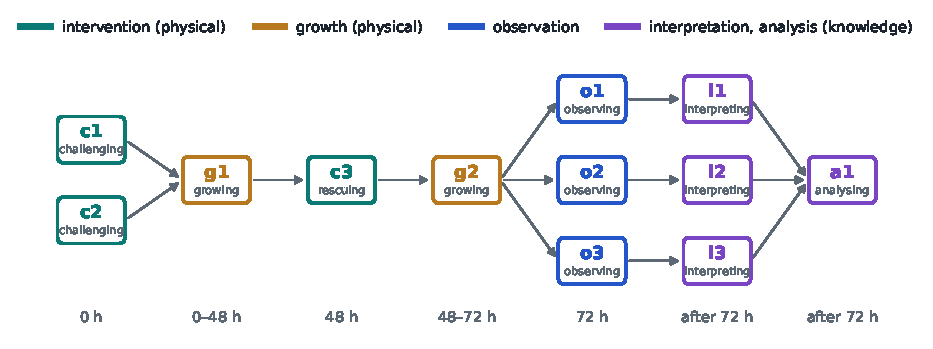
\includegraphics[width=0.85\linewidth,height=0.72\textheight,keepaspectratio]{figures/poset12.pdf}
\caption{Order of the twelve culture actions, derived from causal links over physical (solid) and knowledge (dashed) effects.}\label{fig:poset12}\end{figure}


\subsection{The plan as a CRAM/RPL controller}
The culture plan was then generated as a top-level CRAM/RPL controller: one action plan per culture action type, each
waiting for its requirements, performing its refinement (a lab action designator, or a computation for interpreting
and analysing) and asserting its effects; a partial order of the twelve designators; and a top-level function that
binds the cultures, substances and belief, verifies the given state, runs the plan under the plan's own policies (the
control stays untreated, no contamination, standard environment) and restores the safe state on any exit. The
generator checks that the partial order equals the derived order and that the refinement templates reproduce the lab
designators of the lab-level plan for all eight lab-refined actions. The controller was correct but, as a
representation of the experiment, opaque: the experiment's purpose was dispersed over control structures.


\subsection{The experiment as an entity, and roles}
The third and fourth representations turned the experiment into one entity designator---question, hypotheses,
materials, rules, steps and insights---performed by a one-line top-level plan, \texttt{(perform (an action (type
conducting) (experiment \ldots)))}, whose generic action plan derives everything from the entity. Nesting entity
designators with roles removed all variables: every participant fills a named role, and every later mention is a
definite description that identifies one entity, such as \texttt{(the culture (role rescued))}; steps refer to the
steps they follow by the shortest identifying description. The generator checks that every reference identifies
exactly one step and that the \texttt{after} roles equal the derived order.


\subsection{Organised by the experiment's logic}
Organising the entity by steps still hid the logic. The experiment is three cultures, each defined by its treatment,
kept under shared conditions and observed the same way; comparisons between cultures that differ in exactly one
exposure determine the effects. Rescued and comparator differ only in the rescue, so their difference measures the
rescue's effect; comparator and control differ only in the challenge, so their difference shows that the challenge
injured the cultures---the precondition for there being anything to rescue. Written this way, the twelve actions
follow from the structure and were regenerated exactly, and the second comparison, which the culture plan expressed
only as a requirement of the analysis, became explicit.


\section{The authored experiment designator}\label{sec:authored}
The organised form became the authored source, \texttt{experiment.ldl} (Listing~\ref{lst:xldl}). It has no
variables and no lab entities. The generator \texttt{experiment\_\allowbreak{}designator.py} checks that every comparison isolates
exactly one exposure---the one whose effect it determines---and refuses to proceed otherwise; derives the culture
actions (an intervention per exposure, growth between the treatment times, an observation and an interpretation per
culture, an analysis per comparison, with a licensed comparison's analysis requiring the licensing one's finding);
writes them in the format of the culture plan; and derives their order with the same causal-link machinery.

\begin{Verbatim}[fontsize=\tiny,breaklines,frame=lines,framesep=2mm]
(an experiment
  (instance-of challenge-rescue-experiment)        ; registry/lab/experiment_concepts.ldl; checked by rsa/experiment_concepts.py
  (name challenge-rescue)
  (question (a question
              (asks (which (a recovery-model)))
              (explains (the rescue-efficacy (after (a delay (of 48 h)))))
              (candidate (a recovery-model (name M1_graded)))
              (candidate (a recovery-model (name M2_threshold)))
              (candidate (a recovery-model (name M3_protective)))))
  ;; the design guarantees the gain in expectation (e2m); what one execution yields is measured, not promised
  (goal (the belief (expected-information-gain (>= 0.5 bit))))
  (belief (a belief (over (M1_graded M2_threshold M3_protective)) (prior uniform) (entropy 1.585 bit)))

  ;; what the treatments are made of, and what exposure to them does to a culture
  (substance (a substance (role challenge) (causes (injury rising))))
  (substance (a substance (role rescue) (causes (recovery possible))))

  ;; the cultures: each is defined by its treatment
  (culture (a culture (role rescued) (state baseline)
             (treatment (a treatment
                          (exposure (an exposure (to (the substance (role challenge))) (dose 0.85 au) (at (culture-time 0 h))))
                          (exposure (an exposure (to (the substance (role rescue))) (dose 0.70 au) (at (culture-time 48 h))))))))
  (culture (a culture (role comparator) (state baseline)
             (treatment (a treatment
                          (exposure (an exposure (to (the substance (role challenge))) (dose 0.85 au) (at (culture-time 0 h))))))))
  (culture (a culture (role control) (state baseline)
             (treatment (no treatment))))

  ;; everything but the treatment is shared, so that a difference between cultures is a difference of treatment
  (shared-conditions (a condition
                       (environment culture-standard)
                       (from (culture-time 0 h))
                       (to (culture-time 72 h))
                       (observation (an observation
                                      (readout morphology)
                                      (at (culture-time 72 h))
                                      (side-effect (light-dose increased))      ; imaging is not free (Cell 01 L17)
                                      (interpreted-as (an estimate (quantity organoid-radius) (sigma 2.5 um)))
                                      (needs (a scale (of (an image)) (known true)))))))

  ;; the comparisons: each between two cultures whose treatments differ in exactly one exposure (checked)
  (comparison (a comparison (role validity)
                (between (the culture (role comparator)) (the culture (role control)))
                (determines (the effect (of (the substance (role challenge)))))
                (established-when (the effect (below 0 um) (by-more-than 2 sd)))   ; ILLUSTRATIVE criterion
                (licenses (the comparison (role primary)))))
  (comparison (a comparison (role primary)
                (between (the culture (role rescued)) (the culture (role comparator)))
                (determines (the effect (of (the substance (role rescue)))))
                (updates (the belief))))

  (prevents
    (an exposure (of (the culture (role control))) (to (some substance)))   ; the control stays untreated
    (an event (type contamination) (of (a culture))))
  (maintains
    (each culture (environment culture-standard)))

  ;; what the experiment produces
  (insight (an insight (role answer) (answers (the question)) (form (a posterior (over (the belief))))
             (from (the comparison (role primary)))))
  (insight (an insight (role effect) (of (the substance (role rescue))) (from (the comparison (role primary)))))
  (insight (an insight (role effect) (of (the substance (role challenge))) (from (the comparison (role validity))))))
\end{Verbatim}
\vspace{-4pt}\captionof{listing}{The authored experiment designator (\texttt{rsa/registry/lab/experiment.ldl}).}\label{lst:xldl}\medskip


The derivation yields 13 actions ordered by 15 causal links (7 physical, 8
knowledge): \{x1, x2\} $<$ g1 $<$ x3 $<$ g2 $<$ \{o1, o2, o3\} $<$ \{i1, i2, i3\} $<$ v1 $<$ a1 (Figure~\ref{fig:order13}). Compared with the hand-written plan, all 12 of its actions
are reproduced and one is added, the validity analysis \texttt{v1}; the primary analysis now waits for v1's finding
that the challenge's effect is established, so the belief is not updated unless the challenge worked. The order
changes accordingly: the edges i2$\to$a1, i3$\to$a1 are replaced by i2$\to$v1, i3$\to$v1, v1$\to$a1. Two
effects that the hand-written plan states are not stated in the authored source ((the culture rescued (injury-burden accumulated)); (the culture rescued (viability settled))); neither affects the order.

\begin{figure}[tbp]\centering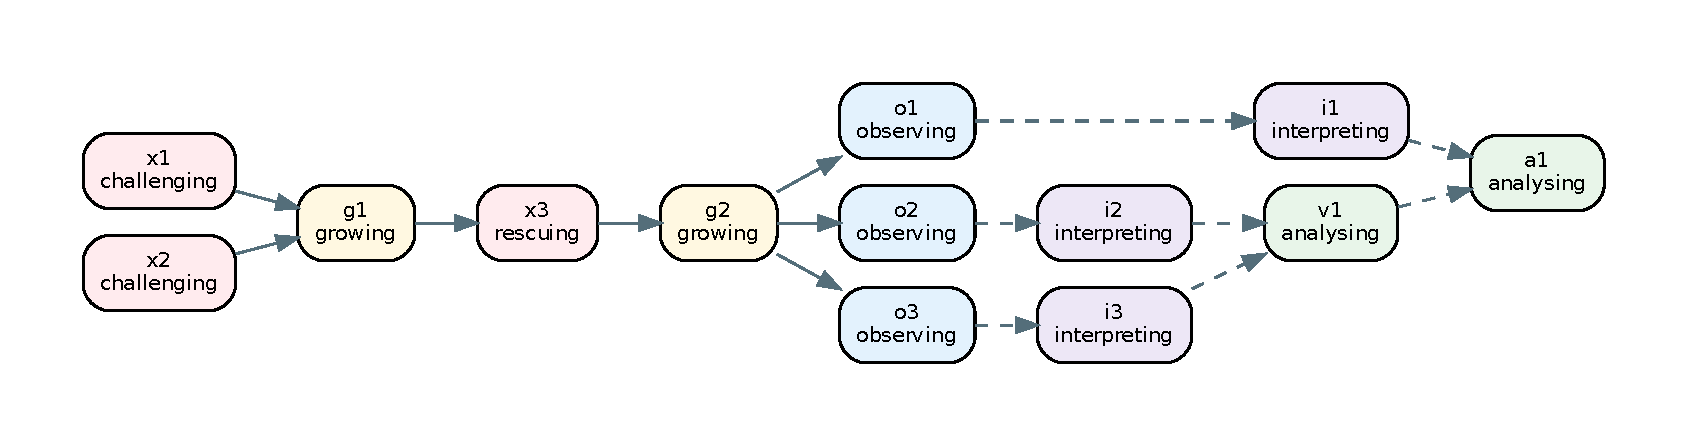
\includegraphics[width=\linewidth,height=0.72\textheight,keepaspectratio]{figures/order13.pdf}
\caption{The 13 culture actions derived from \texttt{experiment.ldl}: interventions (red), growth (yellow), observations (blue), interpretations (violet), analyses (green); solid edges are physical links, dashed edges knowledge links.}\label{fig:order13}\end{figure}


The top-level plan performing the designator is one \texttt{perform} of a \texttt{conducting} action whose
\texttt{experiment} role is filled by the entire designator, enriched with the placement chosen by the mapping to
Cell~01 (plate P17, wells A01, A02, A05), the models' predictions and the checked single differences
(Listing~\ref{lst:top}).

\begin{Verbatim}[fontsize=\scriptsize,breaklines,frame=lines,framesep=2mm]
(def-top-level-cram-function challenge-rescue ()
  (perform (an action
               (type conducting)
               (experiment (an experiment
                               (instance-of challenge-rescue-experiment)
                               (name challenge-rescue)
                               (question (a question
                               ...
\end{Verbatim}
\vspace{-4pt}\captionof{listing}{The head of the top-level plan (\texttt{rsa/out/challenge\_\allowbreak{}rescue\_\allowbreak{}designator.lisp}).}\label{lst:top}\medskip


\section{A conceptual framework for biomedical experiments}\label{sec:framework}
\subsection{Core idea}
\emph{An experiment is a planned process that intervenes on and observes a biological system, executing a design, in
order to change a belief about hypotheses.} The framework keeps four things apart because most errors in practice
come from confusing them: what is \emph{planned} (design and protocol), what \emph{happens} (execution), what is
\emph{measured} (data) and what is \emph{believed} (hypotheses, belief, conclusions). The biology is the hidden state in
between, reached only through interventions and through readouts that are proxies for it. No biological fact or
parameter is asserted by the framework: hypotheses \emph{posit} biology, data are \emph{proxies} (D016).

\begin{figure}[tbp]\centering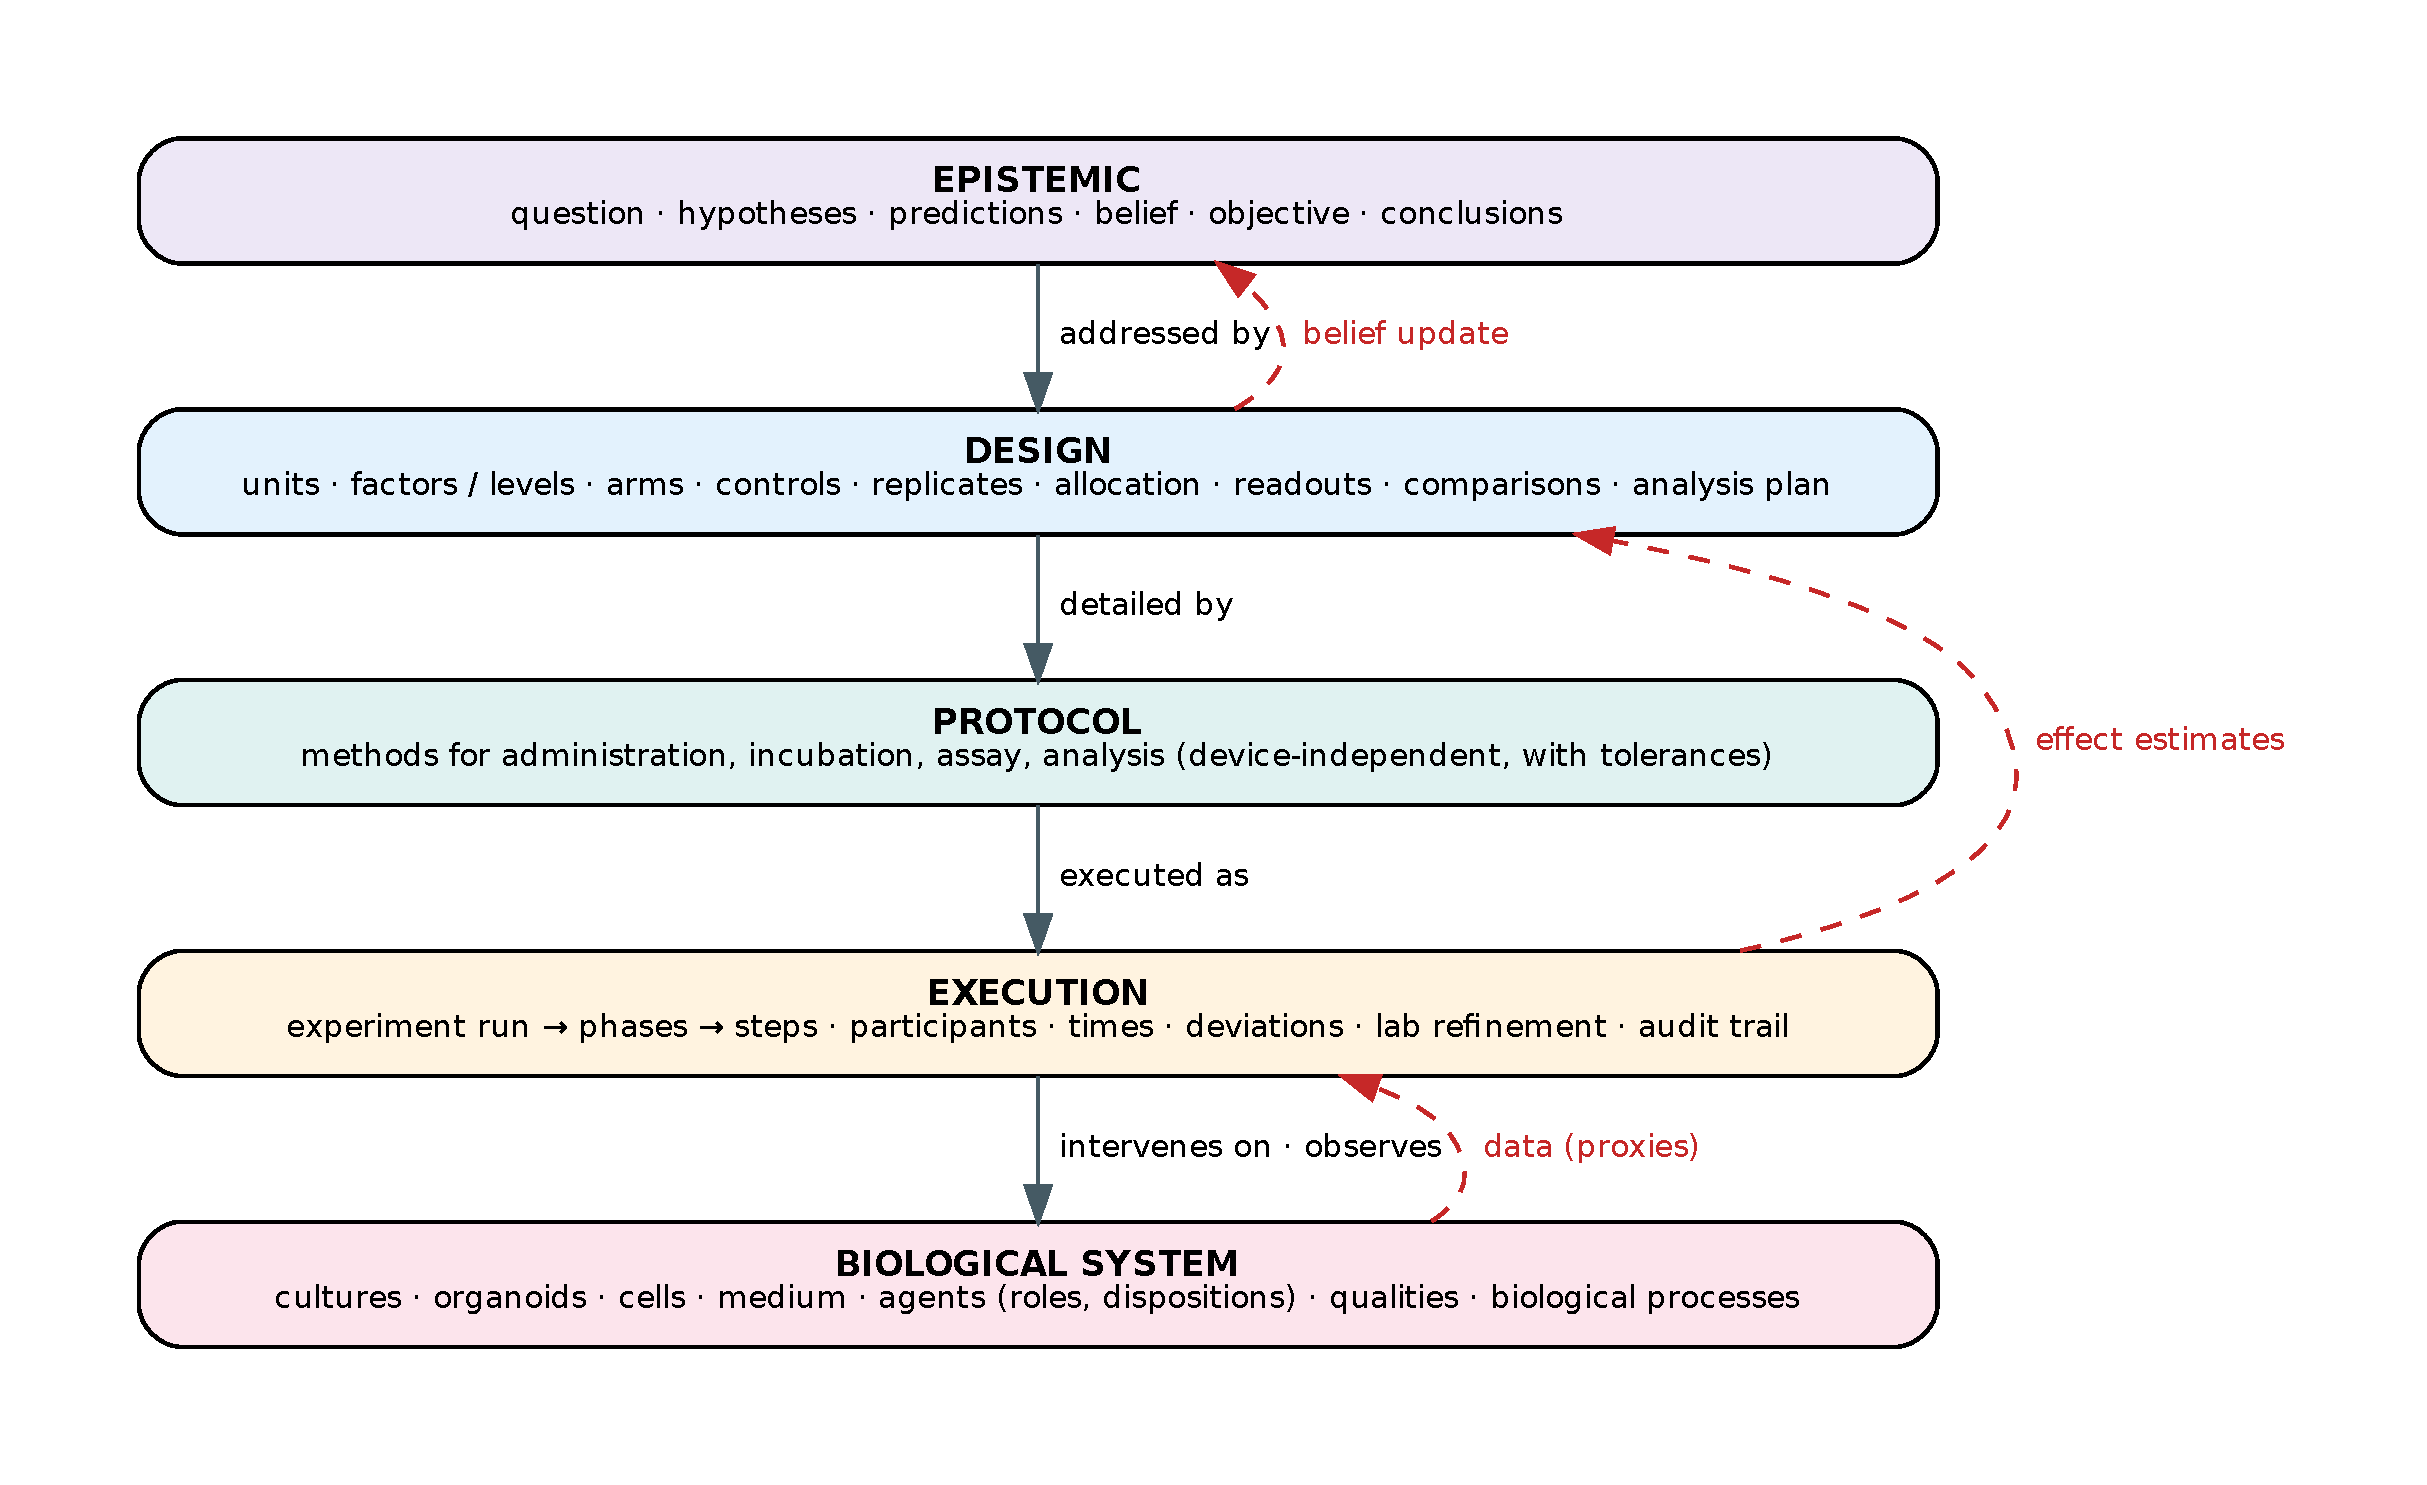
\includegraphics[width=0.95\linewidth,height=0.72\textheight,keepaspectratio]{figures/framework.pdf}
\caption{The five layers of the framework. Downward relations (black) connect the plan to the system; upward relations (red) carry evidence back to the belief.}\label{fig:framework}\end{figure}


\subsection{Five layers}
The \textbf{epistemic layer} holds the question, the competing hypotheses, their predictions, the belief over them,
the objective (here: discriminate the hypotheses with at least a target information gain) and the conclusions. The
\textbf{design layer} holds the units, factors and levels, arms, controls, replication, allocation, readouts,
comparisons and the analysis plan---everything decided before anything is done to a culture. The \textbf{protocol
layer} details each kind of step (how to dose, incubate, image and analyse), device-independent and with tolerances.
The \textbf{execution layer} is the run: phases, steps, participants, times, deviations, the refinement into lab
actions and the audit trail. The \textbf{biological system} is the cultures, organoids, cells, medium, agents with
their roles and dispositions, their qualities, and the biological processes they undergo. Each layer is linked to the
next by one kind of relation (Figure~\ref{fig:framework}): the experiment \emph{executes} the design; steps
\emph{realize} parts of the plan; cultures \emph{participate} in steps; data are \emph{about} qualities and are
\emph{proxies for} hidden states; effect estimates \emph{update} the belief; conclusions are \emph{derived from}
evidence.

\begin{table}[tbp]\centering\small
\caption{Core concepts of the framework.}\label{tab:concepts}
\begin{tabularx}{\linewidth}{@{}p{3.2cm}X@{}}\toprule concept & meaning \\ \midrule
experimental unit & what is treated independently and measured: a culture in a well \\
factor, level & what is varied (agent, dose, time of rescue) and the values it takes \\
treatment & one combination of levels, given as a schedule of administrations \\
arm & a treatment and the units assigned to it; units are members of an arm, not its parts \\
control & an arm defined by what it controls for: negative (untreated, vehicle), positive (expected effect from prior evidence), agent-alone (the agent's own effect), comparator (isolates one factor) \\
replicate & units under the same treatment; biological (independent units) vs.\ technical (repeated measurement) \\
allocation & assignment and placement of units: randomisation, blocking, avoiding edge wells, blinding \\
readout & what is measured, when, by which assay, and what it is a proxy for (size for viability) \\
comparison & a pair of arms whose difference estimates the effect of exactly one factor \\
interaction contrast & a difference of comparisons: whether one factor's effect depends on another \\
validity check & a comparison that licenses another (the injury happened; the agent works) \\
analysis plan & one decision rule per comparison and a rule for deviations, fixed before the run \\
hypothesis, prediction & a model that posits processes, and its expected effect for a comparison \\
belief, information gain & a probability over hypotheses, and how much a design is expected to change it \\
deviation & a difference between execution and plan; it can invalidate comparisons \\
conclusion (insight) & a statement derived from effect estimates and the posterior, with provenance \\
\bottomrule\end{tabularx}\end{table}


\subsection{A multi-axial taxonomy}
Biomedical experiments are classified along independent axes, so the taxonomy is a polyhierarchy rather than a tree:
the \emph{system} (in silico, in vitro---cell line, primary cells, organoid---ex vivo, in vivo, clinical); the
\emph{purpose} (exploratory, confirmatory, hypothesis-discriminating, dose--response, time-course, screening); the
\emph{design structure} (comparative, controlled, factorial, within- or between-unit, randomised, blinded); the
\emph{intervention} (challenge, therapy or rescue, both); and \emph{adequacy} (validated, agent-controlled,
positive-controlled, replicated, pre-specified). Because classes are \emph{defined} rather than merely named, a
reasoner places an experiment under every class it satisfies; the challenge--rescue experiment is, at once, in vitro,
hypothesis-discriminating, a controlled injury--rescue experiment and validated---but not adequately controlled.

\begin{table}[tbp]\centering\small
\caption{Validity criteria and the mechanism that enforces each.}\label{tab:enforce}
\begin{tabularx}{\linewidth}{@{}p{1.9cm}Xp{4.6cm}@{}}\toprule validity & criteria & enforced by \\ \midrule
internal & single factor per comparison; negative, agent-alone and positive controls; randomisation; blinding & defined classes (reasoner); closed-world checks \\
statistical & biological replicates; expected information or power & closed-world counts; information-gain model \\
construct & readout states its proxy relation; manipulation checked by a validity comparison & ontology; licensing order in the plan \\
executional & identity, contamination and environment kept; plan realized; deviations recorded & run-time monitors (CRAM policies); audit trail \\
external & relevance of the system to the target biology & stated as an assumption, never inferred \\
\bottomrule\end{tabularx}\end{table}


\subsection{Criteria and their enforcement}
Table~\ref{tab:enforce} assigns each kind of validity to the mechanism able to enforce it. The principle is a division
of labour: \emph{description logic for what experiments are; closed-world queries for what a design must contain;
run-time monitors for what an execution must keep; probabilistic models for what it will tell us}. A design's
adequacy is thus checked before the run, an execution's integrity during it, and the information it yields after it,
each by the formalism suited to the question.

\subsection{Lifecycle}
The framework is used along a lifecycle: question $\rightarrow$ hypotheses and predictions $\rightarrow$ candidate
designs $\rightarrow$ selection by information and cost $\rightarrow$ \textbf{adequacy check before the run}
$\rightarrow$ protocol $\rightarrow$ refinement into lab actions $\rightarrow$ monitored execution $\rightarrow$ data
$\rightarrow$ analysis by the pre-specified rules $\rightarrow$ belief update $\rightarrow$ conclusions $\rightarrow$ next
question. Each step reads and writes one layer, and the audit trail links them. In the RSA, selection is the
information-gain planner, the adequacy check is the reasoner of Section~\ref{sec:owl} together with the closed-world
queries of Section~\ref{sec:closed}, refinement and execution are the LDL and CRAM layers, and the belief update is
the posterior over the recovery models.

\subsection{Design principles}
Five principles recur. \emph{Plans are information.} A design is an information entity that a process executes;
the same design can be run many times, and each run is classified by its design. \emph{Membership is not
parthood.} A culture is assigned to an arm; it is not part of it, and a level is shared by the arms at that level.
\emph{Roles and dispositions are borne.} An agent is a challenge because it bears that role in this experiment, and a
toxicant because it bears a toxicity disposition; the role is given because of the disposition. \emph{Data are
proxies.} A size datum is about organoid size and is a proxy for viability, never viability itself. \emph{Hypotheses
posit.} A threshold hypothesis posits a loss of recovery capacity; nothing in the ontology asserts that it occurs.


\section{Partonomy}\label{sec:partonomy}
Parthood is the backbone of any representation of experiments, and also its most common source of error: a culture is
not part of an arm, a well is not part of a treatment, an instrument is not part of an assay. The framework therefore
has one transitive parthood relation with three kinds of sub-relations, and keeps every other whole--part-like
relation separate (Table~\ref{tab:partonomy}). Parthood is \emph{kind-preserving}: processes have processes as parts,
material entities material entities, information entities information entities. The kinds of parthood are
\emph{simple} sub-roles of the transitive \emph{hasPart}, so they may be counted (exactly three phases, at most four
arms) without violating the OWL~2 restriction on number restrictions.

\begin{table}[tbp]\centering\footnotesize
\caption{Parthood and the relations kept apart from it.}\label{tab:partonomy}
\begin{tabularx}{\linewidth}{@{}p{3.9cm}p{2.2cm}Xp{3.3cm}@{}}\toprule relation & kind & connects & example \\ \midrule
hasPart & parthood & transitive; kind-preserving & — \\
hasPhase, hasStep & process parthood & experiment $\to$ phases $\to$ steps & cultivation phase has step x1 \\
hasWell, hasOrganoid, hasCell, hasMedium & material parthood & plate $\to$ wells; culture $\to$ organoids, medium & P17 has well A01 \\
hasArm, hasFactor, hasLevel, hasAdministrationSpec, hasComparisonSpec, hasReadout, hasAnalysisPlan, hasDecisionRule & plan parthood & design $\to$ arms, factors, comparisons, readout, analysis plan; arm $\to$ administrations & design has arm rescued \\
contains / containedIn & location & well contains culture; chain containedIn $\circ$ partOf $\sqsubseteq$ locatedIn & A01 contains the rescued culture \\
assignedTo & membership & unit $\to$ arm (functional) & rescued culture assigned to arm rescued \\
atLevel & plan reference & arm $\to$ factor level (shared between arms) & arm rescued at level rescue 0.7au\_\allowbreak{}48h \\
hasParticipant & participation & chain hasPart $\circ$ hasParticipant $\sqsubseteq$ hasParticipant & x1 has input the rescued culture \\
executes & realization & process $\to$ plan part & x1 executes the challenge administration \\
bearerOf / inheresIn & dependence & continuant $\to$ role, disposition, quality & agent bears the challenge role \\
\bottomrule\end{tabularx}\end{table}


Figure~\ref{fig:partonomy} shows the three partonomies of the case study side by side. The process partonomy has the
experiment, its three phases and the 13 steps; the material partonomy has the plate and its three wells, which
\emph{contain} (not have as parts) the three cultures; the plan partonomy has the treatments and their exposures.
Interventions \emph{realize} exposures---the dotted edges---which is how the execution is tied to the plan without
either being part of the other.

\begin{figure}[tbp]\centering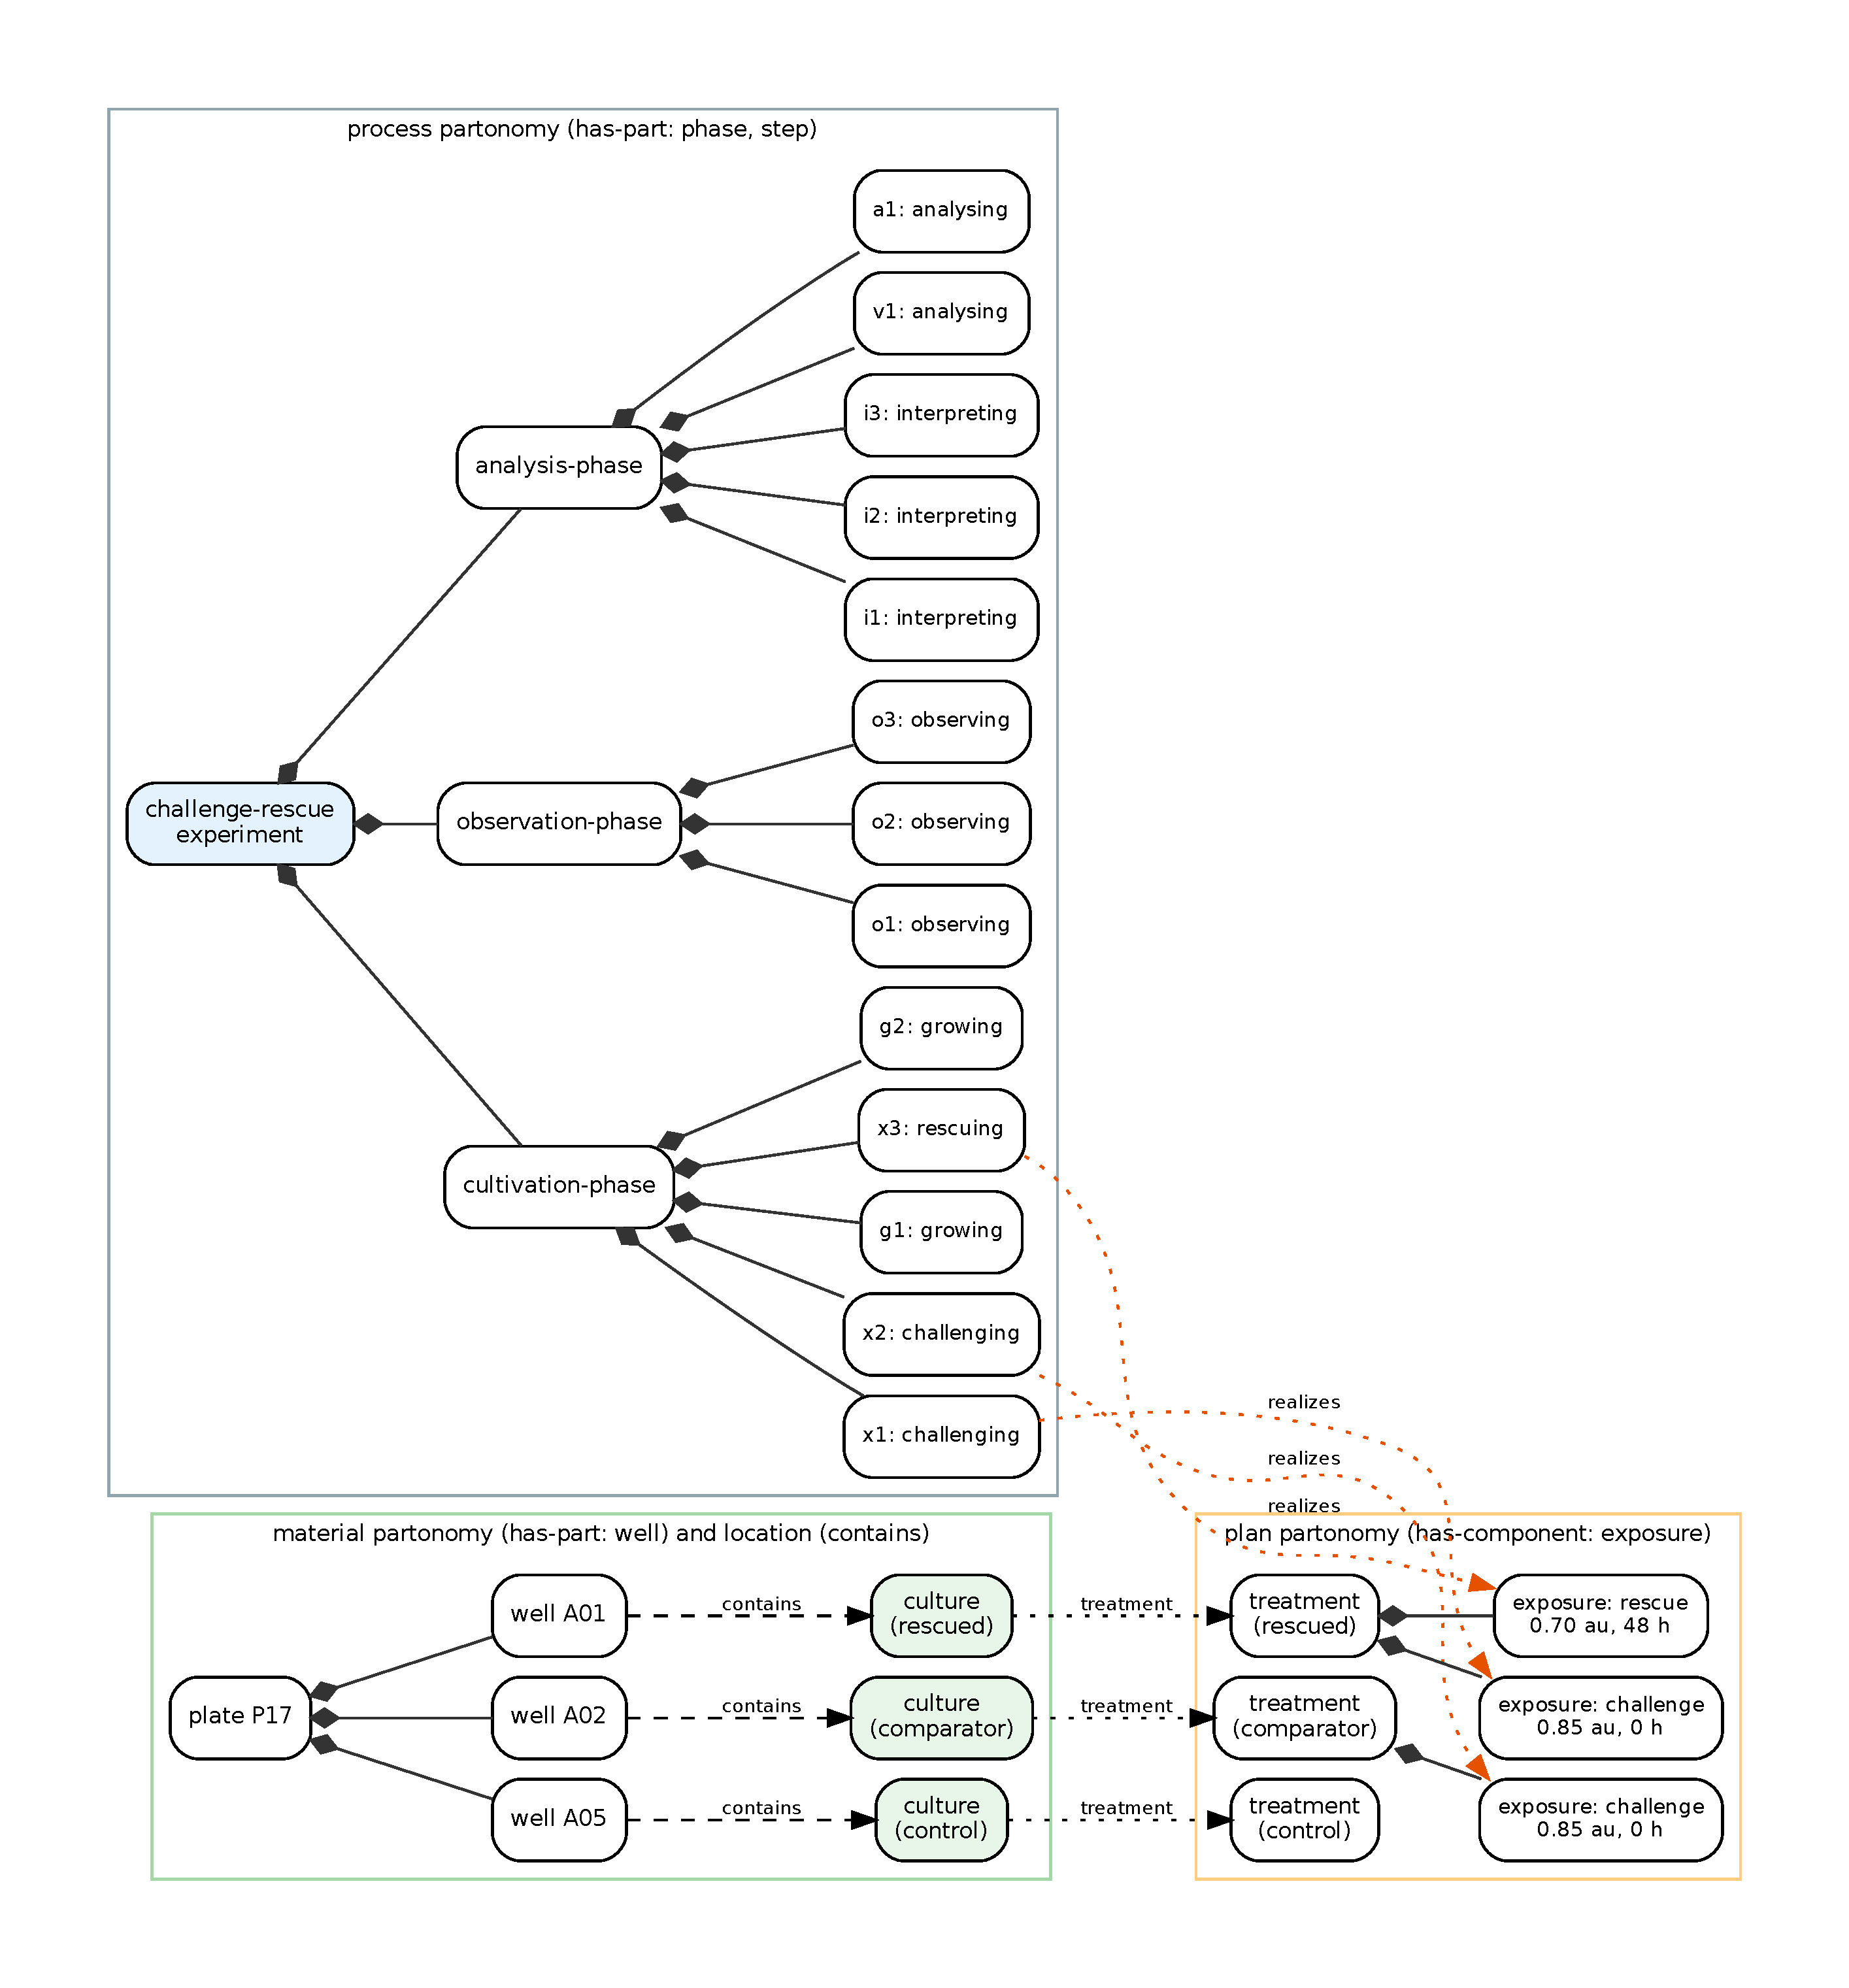
\includegraphics[width=\linewidth,height=0.72\textheight,keepaspectratio]{figures/partonomy.pdf}
\caption{The three partonomies of the case study: process (top), material and location (bottom left), plan (bottom right); dotted edges are realization.}\label{fig:partonomy}\end{figure}


\section{The LDL concept layer}\label{sec:ldlconcepts}
Before the DL axiomatization, the experiment concepts were written in LDL itself
(\texttt{experiment\_\allowbreak{}concepts.ldl}): a specialization hierarchy of 33 concepts with 27 roles,
each concept stating the roles its instances must fill (a pattern and a cardinality), the roles whose fillers are
restricted, and named checks. Five concepts form the experiment hierarchy: \emph{experiment}, then
\emph{comparative} and \emph{hypothesis-discriminating}, then \emph{controlled}, then \emph{challenge--rescue}, which
specializes both branches (Figure~\ref{fig:concepts_v1}). The procedure that derives the actions is attached to
\emph{comparative-experiment} and inherited by every specialization. Listing~\ref{lst:concepts} shows two concepts.

\begin{Verbatim}[fontsize=\scriptsize,breaklines,frame=lines,framesep=2mm]
(a concept controlled-experiment
  (specializes comparative-experiment)
  (documentation "one unit is an untreated control, it stays untreated, and every comparison isolates exactly one
exposure: its two units differ in that exposure only, and it is the exposure whose effect the comparison determines")
  (has unit (an entity (role control) (treatment (no treatment))) (exactly 1))
  (has prevents (an exposure (of (the culture (role control)))) (at-least 1))
  (check single-difference))

(a concept challenge-rescue-experiment
  (specializes controlled-experiment hypothesis-discriminating-experiment)
  (documentation "units are injured by a challenge; one is then given a rescue after a delay. A validity comparison
(comparator vs control) establishes the challenge's effect and licenses the primary comparison (rescued vs
comparator), which determines the rescue's effect and updates the belief over models of recovery")
  (has substance (a substance (role challenge)) (exactly 1))
  (has substance (a substance (role rescue)) (exactly 1))
  (has unit (a culture (role rescued)
              (treatment (a treatment (exposure (an exposure (to (the substance (role challenge)))))
                                      (exposure (an exposure (to (the substance (role rescue))))))))
       (exactly 1))
  (has unit (a culture (role comparator) (treatment (a treatment (exposure (an exposure (to (the substance (role challenge))))))))
       (exactly 1))
  (has comparison (a comparison (role validity) (between (the culture (role comparator)) (the culture (role control)))
                    (determines (the effect (of (the substance (role challenge))))) (licenses (the comparison (role primary))))
       (exactly 1))
  (has comparison (a comparison (role primary) (between (the culture (role rescued)) (the culture (role comparator)))
                    (determines (the effect (of (the substance (role rescue))))) (updates (the belief)))
       (exactly 1))
  (check rescue-after-challenge))
\end{Verbatim}
\vspace{-4pt}\captionof{listing}{Two concepts of the LDL concept layer (\texttt{experiment\_\allowbreak{}concepts.ldl}).}\label{lst:concepts}\medskip


The checker \texttt{experiment\_\allowbreak{}concepts.py} verifies the experiment \emph{as derived and placed}---with its phases and
steps from the procedure and its plate and wells from the mapping---against its concept and all ancestors, checks
every part against its own concept (50/50 parts conform), and classifies it independently. The declared concept
is confirmed as the most specific one; all 36 constraints hold (Table~\ref{tab:v1conf}). Each of the
8 negative controls---modified copies of the design or of its derived plan---fails exactly at the level
whose constraint it breaks and is reclassified under the more general concepts it still satisfies
(Table~\ref{tab:v1neg}).

\begin{table}[tbp]\centering\small
\caption{Conformance of the experiment to the LDL concept hierarchy.}\label{tab:v1conf}
\begin{tabularx}{\linewidth}{@{}Xp{2.4cm}p{2.2cm}@{}}\toprule concept & constraints & satisfied \\ \midrule
experiment & 4 & 4 \\
comparative-experiment & 17 & 17 \\
controlled-experiment & 3 & 3 \\
hypothesis-discriminating-experiment & 5 & 5 \\
challenge-rescue-experiment & 7 & 7 \\
\bottomrule\end{tabularx}\end{table}

\begin{table}[tbp]\centering\footnotesize
\caption{Negative controls of the LDL concept layer.}\label{tab:v1neg}
\begin{tabularx}{\linewidth}{@{}p{4.8cm}XX@{}}\toprule modification & fails at & still an instance of \\ \midrule
comparator dose 0.60 au & controlled-experiment & hypothesis-discriminating-experiment, comparative-experiment \\
control culture removed & comparative-experiment, controlled-experiment & hypothesis-discriminating-experiment \\
rescue given with the challenge (0 h) & challenge-rescue-experiment & hypothesis-discriminating-experiment, controlled-experiment \\
belief and answer removed & hypothesis-discriminating-experiment & controlled-experiment \\
rescue intervention missing from the plan & comparative-experiment & hypothesis-discriminating-experiment \\
comparator on another plate & comparative-experiment & hypothesis-discriminating-experiment \\
an observation step in two phases & comparative-experiment & hypothesis-discriminating-experiment \\
a well as part of a treatment & experiment, comparative-experiment & --- \\
\bottomrule\end{tabularx}\end{table}

\begin{figure}[tbp]\centering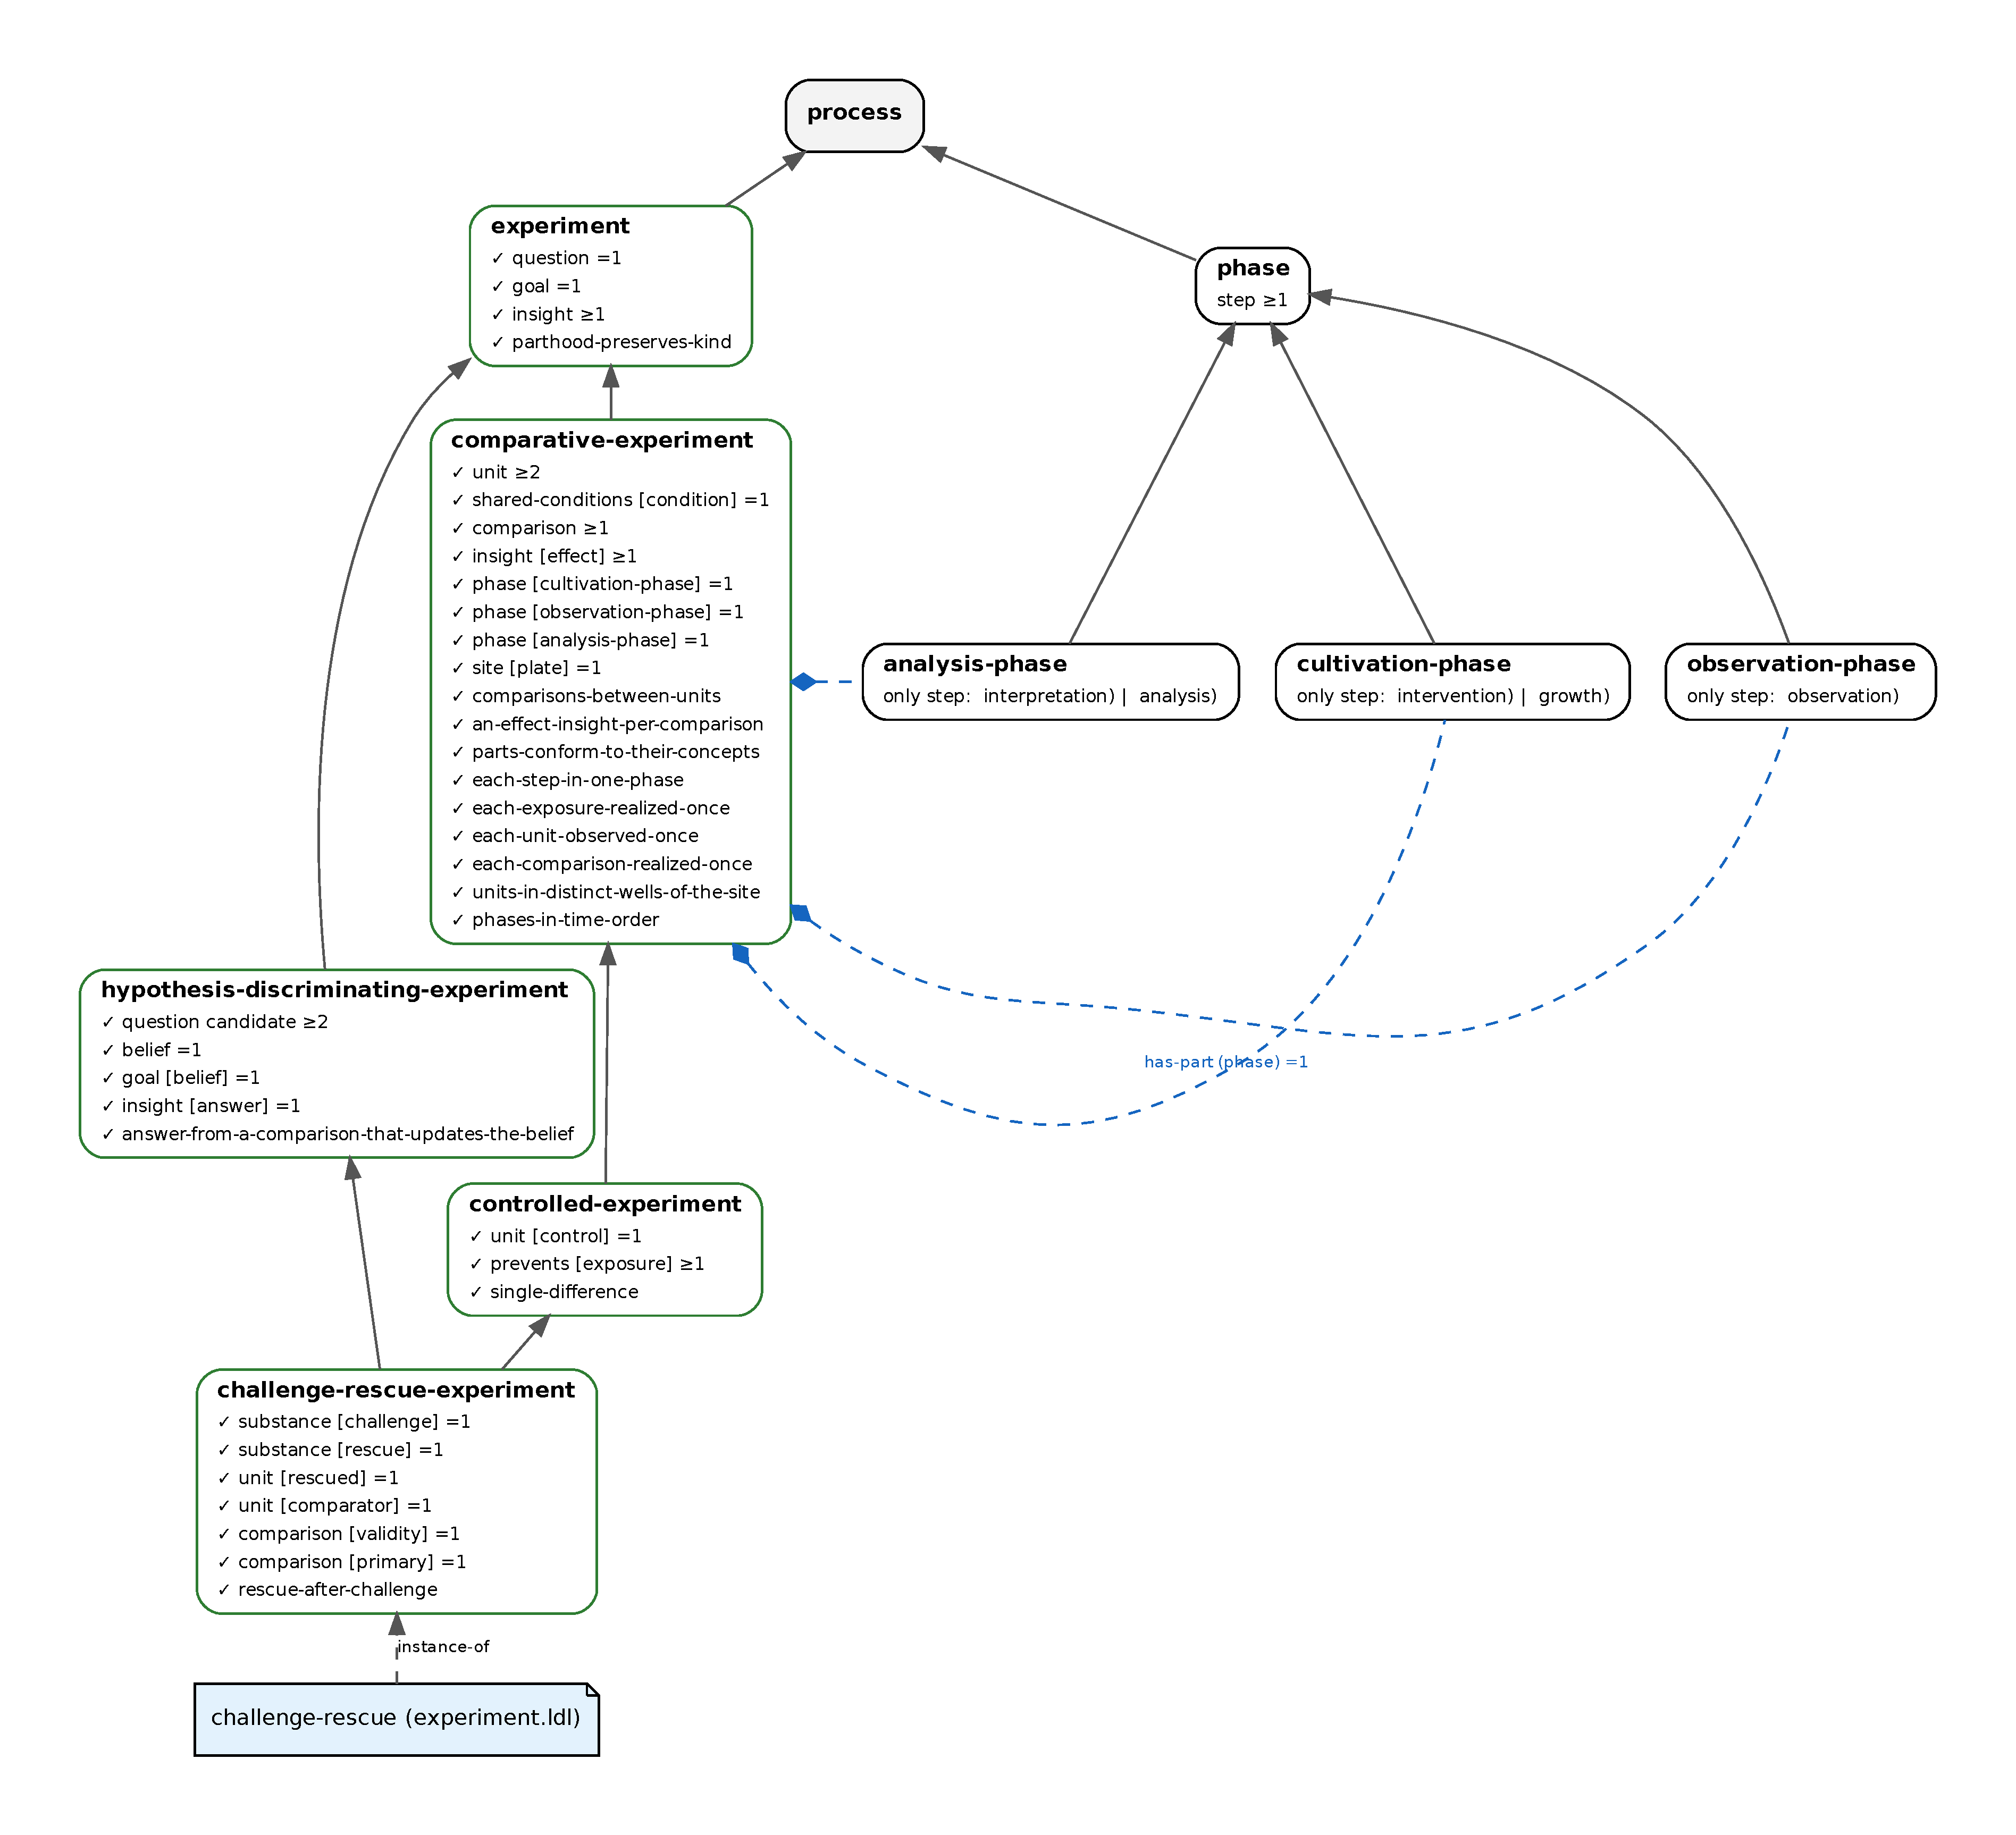
\includegraphics[width=0.9\linewidth,height=0.72\textheight,keepaspectratio]{figures/concepts_v1.pdf}
\caption{The LDL concept hierarchy with each concept's own constraints, checked against the experiment; the instance is declared \texttt{instance-of} challenge-rescue-experiment.}\label{fig:concepts_v1}\end{figure}


\section{A first description-logic statement}\label{sec:dlv1}
The first DL statement (\texttt{experiment\_\allowbreak{}dl.py}) was generated from the LDL concept file: each \texttt{has}
clause became a qualified number restriction, each \texttt{only} clause a value restriction, a pattern's slots nested
existentials, and \texttt{(role $x$)} the restriction $\exists \mathit{hasRole}.X\mathit{Role}$. Because it was
generated, it could not drift from what the checker checks. Its main value was diagnostic: stating each named check
in the logic it needs (Table~\ref{tab:v1expr}) showed which parts of the experiment concept OWL~2 can carry and which
it cannot. Single difference compares two individuals' sets of exposures and needs first-order logic with counting;
``rescue after challenge'' and the order of phases compare data values reached by different paths and need concrete
domains with feature chains \citep{baader1991}; ``all units on one plate'' is a role-value map, undecidable together
with the rest. The generator also verified that number restrictions are placed only on simple roles.

The first statement had three weaknesses that the second axiomatization removes: the design and the experiment were
one entity, so a plan and its execution could not be told apart; roles were values of a \emph{hasRole} slot rather
than realizable entities borne by participants; and the concepts were \emph{primitive}, so nothing was classified---the
hierarchy was only checked against what was declared.

\begin{table}[tbp]\centering\footnotesize
\caption{Expressivity of the named checks of the LDL concept layer.}\label{tab:v1expr}
\begin{tabularx}{\linewidth}{@{}p{5.2cm}X@{}}\toprule constraint & logic it needs \\ \midrule
parthood-preserves-kind & OWL 2 DL \\
answer-from-a-comparison-that-updates-the-belief & OWL 2 DL \\
comparisons-between-units & SROIQ role inclusion \\
an-effect-insight-per-comparison & FOL \\
parts-conform-to-their-concepts & DL semantics \\
each-step-in-one-phase & OWL 2 DL \\
each-exposure-realized-once & OWL 2 DL + rule \\
each-unit-observed-once & FOL \\
each-comparison-realized-once & OWL 2 DL + rule \\
units-in-distinct-wells-of-the-site & FOL (path agreement) \\
phases-in-time-order & ALC(D) feature chains \\
single-difference & FOL with counting \\
rescue-after-challenge & ALC(D) feature chains \\
\bottomrule\end{tabularx}\end{table}


\section{The OWL~2~DL axiomatization}\label{sec:owl}
The second axiomatization (\texttt{experiment\_\allowbreak{}ontology.py}) states the framework as a biomedical ontology in
$\mathcal{SROIQ}(\mathbf{D})$. It is written once, in a small DL syntax embedded in Python, and rendered three ways:
as DL notation (this report and Appendix~\ref{app:tbox}), as OWL functional syntax (\texttt{experiment.ofn}) and as
an Owlready2 ontology \citep{lamy2017} over which HermiT \citep{glimm2014} reasons. It has 246 TBox axioms over
174 concepts, 52 object properties and 12 data properties, in 13 groups
(Table~\ref{tab:tbox}); 71 axioms are definitions ($\equiv$), which is what lets the reasoner classify. The
namespace is \texttt{https://aicor.example/okf/experiment\#}. This section presents the axioms that carry the
framework; the full TBox is in Appendix~\ref{app:tbox}.

\begin{table}[tbp]\centering\small
\caption{The TBox by group.}\label{tab:tbox}
\begin{tabularx}{\linewidth}{@{}Xp{2.2cm}p{2.2cm}@{}}\toprule group & axioms & definitions \\ \midrule
Upper level & 21 & 0 \\
Relations and partonomy & 41 & 0 \\
Biological material and labware & 24 & 5 \\
Biological processes & 7 & 0 \\
Plans: designs, arms, administrations, comparisons & 20 & 15 \\
Factors, levels and treatments & 14 & 4 \\
Controls & 6 & 4 \\
Readouts and analysis plan & 17 & 4 \\
Design classes & 10 & 10 \\
Experiments, phases and steps & 26 & 10 \\
Data, hypotheses and conclusions & 12 & 0 \\
Laboratories, devices and capabilities & 35 & 12 \\
Design requirements & 13 & 7 \\
\bottomrule\end{tabularx}\end{table}


\subsection{Upper level and partonomy}
Continuants and occurrents are disjoint; material entities, specifically dependent continuants (qualities and
realizable entities) and information content entities are disjoint; roles and dispositions are disjoint realizable
entities; planned and biological processes are disjoint. Parthood is transitive and kind-preserving:

\ax{\mathrm{Trans}(\mathit{hasPart})}
\ax{\mathsf{Process} ⊑ ∀\mathit{hasPart}.\mathsf{Process}}
\ax{\mathsf{MaterialEntity} ⊑ ∀\mathit{hasPart}.\mathsf{MaterialEntity}}
\ax{\mathsf{InformationContentEntity} ⊑ ∀\mathit{hasPart}.\mathsf{InformationContentEntity}}
\ax{\mathit{containedIn} ∘ \mathit{partOf} ⊑ \mathit{locatedIn}}
\ax{\mathit{hasPart} ∘ \mathit{hasParticipant} ⊑ \mathit{hasParticipant}}

The bearer relation ranges over specifically dependent continuants---qualities as well as roles and dispositions. An
earlier version restricted it to realizable entities, which made organoid size, every size datum and the executed
experiment's ABox unsatisfiable; HermiT found the error at the first run, and the negative controls were guarded so
that they count only against a consistent base.

\subsection{Biological material, agents and units}

\ax{\mathsf{OrganoidCulture} ⊑ \mathsf{MaterialEntity} ⊓\allowbreak ∃\mathit{hasOrganoid}.\mathsf{Organoid} ⊓\allowbreak ∃\mathit{hasMedium}.\mathsf{CultureMedium}}
\ax{\mathsf{Organoid} ⊑ \mathsf{MaterialEntity} ⊓\allowbreak ∃\mathit{hasCell}.\mathsf{Cell}}
\ax{\mathsf{Well} ⊑ \mathsf{MaterialEntity} ⊓\allowbreak (≤1 \mathit{contains}.\mathsf{OrganoidCulture})}
\ax{\mathsf{RecoveryCapacity} ⊑ \mathsf{Disposition} ⊓\allowbreak ∃\mathit{inheresIn}.\mathsf{OrganoidCulture} ⊓\allowbreak ∀\mathit{realizedIn}.\mathsf{RecoveryProcess}}
\ax{\mathsf{ToxicityDisposition} ⊑ \mathsf{Disposition} ⊓\allowbreak ∃\mathit{inheresIn}.\mathsf{ChemicalAgent} ⊓\allowbreak ∀\mathit{realizedIn}.\mathsf{InjuryProcess}}
\ax{\mathsf{Toxicant} ≡ \mathsf{ChemicalAgent} ⊓\allowbreak ∃\mathit{bearerOf}.\mathsf{ToxicityDisposition}}
\ax{\mathsf{ChallengeAgent} ≡ \mathsf{ChemicalAgent} ⊓\allowbreak ∃\mathit{bearerOf}.\mathsf{ChallengeAgentRole}}
\ax{\mathsf{ChallengeAgent} ⊑ \mathsf{Toxicant}}
\ax{\mathsf{ExperimentalUnit} ≡ \mathsf{OrganoidCulture} ⊓\allowbreak ∃\mathit{bearerOf}.\mathsf{ExperimentalUnitRole}}

An organoid culture is organoids in medium; a well holds at most one culture. Agents are chemical entities defined by
the roles they bear in the experiment; the challenge agent is a toxicant because its role is given for its toxicity
disposition. An experimental unit is an organoid culture bearing the experimental-unit role. Recovery capacity and
toxicity are dispositions realized only in recovery and injury processes, respectively.

\subsection{Arms, defined by their treatment}
An arm's class follows from what it administers. With the closure axioms of Section~\ref{sec:closed}, the reasoner
infers these classes from an arm's administration specifications alone:

\ax{\mathsf{UntreatedArm} ≡ \mathsf{ArmSpecification} ⊓\allowbreak ¬∃\mathit{hasAdministrationSpec}.\mathsf{AdministrationSpecification}}
\ax{\mathsf{VehicleControlArm} ≡ \mathsf{ArmSpecification} ⊓\allowbreak ∃\mathit{hasAdministrationSpec}.\mathsf{VehicleSpec} ⊓\allowbreak ¬∃\mathit{hasAdministrationSpec}.(\mathsf{ChallengeSpec} ⊔\allowbreak \mathsf{RescueSpec})}
\ax{\mathsf{NegativeControlArm} ≡ \mathsf{UntreatedArm} ⊔\allowbreak \mathsf{VehicleControlArm}}
\ax{\mathsf{ChallengeOnlyArm} ≡ \mathsf{ArmSpecification} ⊓\allowbreak ∃\mathit{hasAdministrationSpec}.\mathsf{ChallengeSpec} ⊓\allowbreak ¬∃\mathit{hasAdministrationSpec}.\mathsf{RescueSpec}}
\ax{\mathsf{RescueOnlyArm} ≡ \mathsf{ArmSpecification} ⊓\allowbreak ∃\mathit{hasAdministrationSpec}.\mathsf{RescueSpec} ⊓\allowbreak ¬∃\mathit{hasAdministrationSpec}.\mathsf{ChallengeSpec}}
\ax{\mathsf{ChallengeRescueArm} ≡ \mathsf{ArmSpecification} ⊓\allowbreak ∃\mathit{hasAdministrationSpec}.\mathsf{ChallengeSpec} ⊓\allowbreak ∃\mathit{hasAdministrationSpec}.\mathsf{RescueSpec}}
\ax{\mathsf{ReplicatedArm} ≡ \mathsf{ArmSpecification} ⊓\allowbreak (≥3 \mathit{hasAssignedUnit}.\mathsf{ExperimentalUnit})}
\ax{\mathsf{PositiveControlArm} ≡ \mathsf{ArmSpecification} ⊓\allowbreak ∃\mathit{hasExpectedOutcome}.\mathsf{EvidenceBasedExpectation}}

\subsection{Factors, levels and comparisons}
A factor has at least two levels; an arm is at one level of each factor; a comparison contrasts the factors in which
its arms differ. A comparison is classified by the arms it compares:

\ax{\mathsf{InjuryValidityComparison} ≡ \mathsf{ComparisonSpecification} ⊓\allowbreak ∃\mathit{compares}.\mathsf{ChallengeOnlyArm} ⊓\allowbreak ∃\mathit{compares}.\mathsf{NegativeControlArm}}
\ax{\mathsf{RescueEffectComparison} ≡ \mathsf{ComparisonSpecification} ⊓\allowbreak ∃\mathit{compares}.\mathsf{ChallengeRescueArm} ⊓\allowbreak ∃\mathit{compares}.\mathsf{ChallengeOnlyArm}}
\ax{\mathsf{AgentAloneComparison} ≡ \mathsf{ComparisonSpecification} ⊓\allowbreak ∃\mathit{compares}.\mathsf{RescueOnlyArm} ⊓\allowbreak ∃\mathit{compares}.\mathsf{NegativeControlArm}}
\ax{\mathsf{RescueTimingComparison} ≡ \mathsf{ComparisonSpecification} ⊓\allowbreak (=2 \mathit{compares}.\mathsf{ChallengeRescueArm})}
\ax{\mathsf{Factor} ⊑ \mathsf{PlanSpecification} ⊓\allowbreak (≥2 \mathit{hasLevel}.\mathsf{FactorLevel})}
\ax{\mathsf{FactorLevel} ⊑ \mathsf{PlanSpecification} ⊓\allowbreak (=1 \mathit{levelOf}.\mathsf{Factor})}
\ax{\mathsf{SingleFactorComparison} ≡ \mathsf{ComparisonSpecification} ⊓\allowbreak (=1 \mathit{contrasts}.\mathsf{Factor})}
\ax{\mathsf{InteractionContrast} ⊑ \mathsf{PlanSpecification} ⊓\allowbreak (=2 \mathit{differenceOf}.\mathsf{ComparisonSpecification})}
\ax{\mathsf{PositiveControlComparison} ≡ \mathsf{ComparisonSpecification} ⊓\allowbreak ∃\mathit{compares}.\mathsf{PositiveControlArm} ⊓\allowbreak ∃\mathit{compares}.\mathsf{ChallengeOnlyArm}}

\subsection{Readouts and the analysis plan}
A readout measures a quality at a time and may be a proxy for another. The analysis plan has decision rules; a
comparison rule applies to exactly one comparison; a deviation rule applies to none. A design is pre-specified when it
has a readout, an analysis plan, and every comparison is covered by a rule:

\ax{\mathsf{ReadoutSpecification} ⊑ \mathsf{PlanSpecification} ⊓\allowbreak ∃\mathit{measures}.\mathsf{Quality} ⊓\allowbreak ∃\mathit{atTime_h}.\mathsf{decimal}}
\ax{\mathsf{SizeReadout} ≡ \mathsf{ReadoutSpecification} ⊓\allowbreak ∃\mathit{measures}.\mathsf{OrganoidSize} ⊓\allowbreak ∃\mathit{isProxyFor}.\mathsf{Viability}}
\ax{\mathsf{ComparisonRule} ⊑ \mathsf{DecisionRule} ⊓\allowbreak (=1 \mathit{appliesTo}.\mathsf{ComparisonSpecification})}
\ax{\mathsf{BayesianUpdateRule} ⊑ \mathsf{ComparisonRule} ⊓\allowbreak (≥2 \mathit{isAbout}.\mathsf{Hypothesis})}
\ax{\mathsf{DeviationRule} ⊑ \mathsf{DecisionRule} ⊓\allowbreak ¬∃\mathit{appliesTo}.⊤}
\ax{\mathsf{CoveredComparison} ≡ \mathsf{ComparisonSpecification} ⊓\allowbreak ∃\mathit{appliesTo}^{-}.\mathsf{ComparisonRule}}
\ax{\mathsf{PreSpecifiedDesign} ≡ \mathsf{StudyDesign} ⊓\allowbreak ∃\mathit{hasReadout}.\mathsf{ReadoutSpecification} ⊓\allowbreak ∃\mathit{hasAnalysisPlan}.\mathsf{AnalysisPlan} ⊓\allowbreak ∀\mathit{hasComparisonSpec}.\mathsf{CoveredComparison}}

\subsection{Design and experiment classes}
Design classes are defined by arms, comparisons, factors and the analysis plan. Adequate control---the reviewer's
standard---is the conjunction of agent control, a positive control, replication, single-factor comparisons and a
pre-specified analysis. Experiment classes mirror design classes: an investigation executes exactly one design and is
classified by it.

\ax{\mathsf{WellContrastedDesign} ≡ \mathsf{StudyDesign} ⊓\allowbreak ∀\mathit{hasComparisonSpec}.\mathsf{SingleFactorComparison}}
\ax{\mathsf{ControlledDesign} ≡ \mathsf{ComparativeDesign} ⊓\allowbreak ∃\mathit{hasArm}.\mathsf{NegativeControlArm}}
\ax{\mathsf{InjuryRescueDesign} ≡ \mathsf{ControlledDesign} ⊓\allowbreak ∃\mathit{hasArm}.\mathsf{ChallengeRescueArm} ⊓\allowbreak ∃\mathit{hasArm}.\mathsf{ChallengeOnlyArm} ⊓\allowbreak ∃\mathit{hasComparisonSpec}.\mathsf{RescueEffectComparison}}
\ax{\mathsf{ValidatedInjuryRescueDesign} ≡ \mathsf{InjuryRescueDesign} ⊓\allowbreak ∃\mathit{hasComparisonSpec}.\mathsf{InjuryValidityComparison}}
\ax{\mathsf{AgentControlledInjuryRescueDesign} ≡ \mathsf{ValidatedInjuryRescueDesign} ⊓\allowbreak ∃\mathit{hasArm}.\mathsf{RescueOnlyArm} ⊓\allowbreak ∃\mathit{hasArm}.\mathsf{VehicleControlArm} ⊓\allowbreak ∃\mathit{hasComparisonSpec}.\mathsf{AgentAloneComparison}}
\ax{\mathsf{TherapeuticWindowDesign} ≡ \mathsf{InjuryRescueDesign} ⊓\allowbreak (≥2 \mathit{hasArm}.\mathsf{ChallengeRescueArm})}
\ax{\mathsf{ReplicatedDesign} ≡ \mathsf{StudyDesign} ⊓\allowbreak ∀\mathit{hasArm}.\mathsf{ReplicatedArm}}
\ax{\mathsf{AdequatelyControlledInjuryRescueDesign} ≡ \mathsf{AgentControlledInjuryRescueDesign} ⊓\allowbreak \mathsf{PositiveControlledDesign} ⊓\allowbreak \mathsf{ReplicatedDesign} ⊓\allowbreak \mathsf{WellContrastedDesign} ⊓\allowbreak \mathsf{PreSpecifiedDesign}}
\ax{\mathsf{SufficientlyInformativeDesign} ≡ \mathsf{StudyDesign} ⊓\allowbreak ∃\mathit{expectedInformationGain_bits}.\mathsf{decimal}_{\geq 0.5}}
\ax{\mathsf{Investigation} ⊑ \mathsf{PlannedProcess} ⊓\allowbreak (=1 \mathit{executes}.\mathsf{StudyDesign})}
\ax{\mathsf{ValidatedInjuryRescueExperiment} ≡ \mathsf{Investigation} ⊓\allowbreak ∃\mathit{executes}.\mathsf{ValidatedInjuryRescueDesign}}

\subsection{Phases, steps, data and hypotheses}
A comparative experiment has exactly one cultivation, observation and analysis phase; each phase restricts its steps
(administrations and incubations; assays; data transformations). A size datum is about organoid size and a proxy for
viability. The recovery hypotheses are distinguished by what they posit:

\ax{\mathsf{ComparativeExperiment} ≡ \mathsf{Investigation} ⊓\allowbreak ∃\mathit{executes}.\mathsf{ComparativeDesign}}
\ax{\mathsf{ComparativeExperiment} ⊑ (=1 \mathit{hasPhase}.\mathsf{CultivationPhase}) ⊓\allowbreak (=1 \mathit{hasPhase}.\mathsf{ObservationPhase}) ⊓\allowbreak (=1 \mathit{hasPhase}.\mathsf{AnalysisPhase})}
\ax{\mathsf{CultivationPhase} ⊑ \mathsf{Phase} ⊓\allowbreak ∀\mathit{hasStep}.(\mathsf{Administration} ⊔\allowbreak \mathsf{Incubation})}
\ax{\mathsf{SizeDatum} ⊑ \mathsf{MeasurementDatum} ⊓\allowbreak ∃\mathit{isAbout}.\mathsf{OrganoidSize} ⊓\allowbreak ∃\mathit{isProxyFor}.\mathsf{Viability}}
\ax{\mathsf{GradedRecoveryHypothesis} ⊑ \mathsf{RecoveryHypothesis} ⊓\allowbreak ¬∃\mathit{posits}.\mathsf{LossOfRecoveryCapacity}}
\ax{\mathsf{ThresholdRecoveryHypothesis} ⊑ \mathsf{RecoveryHypothesis} ⊓\allowbreak ∃\mathit{posits}.\mathsf{LossOfRecoveryCapacity}}
\ax{\mathsf{ProtectiveResponseHypothesis} ⊑ \mathsf{ThresholdRecoveryHypothesis} ⊓\allowbreak ∃\mathit{posits}.(\mathsf{ProtectiveResponse} ⊓\allowbreak ∃\mathit{delays}.\mathsf{LossOfRecoveryCapacity})}

\subsection{Alignment to Cell~01's biology ontology}
Where a concept means the same as one of Cell~01's biology ontology (\texttt{aicor-biology.ttl}, read only), it is
subsumed by it: 17 axioms such as $\mathsf{Organoid} \sqsubseteq \mathsf{bio{:}Organoid}$,
$\mathsf{ChallengeAdministration} \sqsubseteq \mathsf{bio{:}ControlledToxicChallenge}$ and
$\mathsf{ImagingAssay} \sqsubseteq \mathsf{bio{:}ImagingProcess}$. Concepts whose meaning differs (the biology
ontology's models are scientific models, ours are hypotheses that posit processes) are not aligned. Reasoning over both
ontologies together is consistent with no unsatisfiable concept (HermiT 0.63~s).


\section{Closure and the closed world}\label{sec:closed}
\subsection{Closure axioms}
OWL reasons under the open world. That an arm has a challenge and \emph{no} rescue cannot be concluded from the absence
of a rescue assertion, and the definitions of Section~\ref{sec:owl} contain negations and universal restrictions. The
ABox therefore closes what the design states: every arm has at most as many administrations and assigned units as it
lists, the design at most as many arms and comparisons, and each comparison at most as many contrasted factors.
Together with distinctness assertions, these let HermiT conclude, for example, that the comparator arm---one
administration, which is a challenge specification, disjoint from rescue specifications---is a challenge-only arm, and
that a design all of whose (closed) arms are replicated satisfies $\forall \mathit{hasArm}.\mathsf{ReplicatedArm}$.
The closure of the design's arms had at first been stated over arm specifications only; under the open world another
kind of filler remained possible and the universal restriction could not be concluded, so the closure now ranges over
every filler.

\subsection{Closed-world checks}
What OWL~2 cannot state, or cannot conclude under the open world, is checked by queries over the design as given:
every arm has one level of each factor; each comparison contrasts exactly one factor; the administration schedules of
compared arms differ only at time points belonging to the contrasted factor (vehicle matching); whether the design is a
full factorial (information, not a requirement); whether some interaction is estimable (a complete $2\times2$
sub-table of two factors' levels); every comparison has a decision rule; a positive control licenses the primary
comparison; at least 3 replicates per arm (an ILLUSTRATIVE criterion); units off the plate edge; all units
on one plate; and, for an executed experiment, each administration specification executed exactly once. The
single-factor check replaces the earlier time-point check: the therapeutic-window comparison (late vs.\ early rescue)
differs at two time points but in one factor, the time of rescue.


\section{Reasoning results}\label{sec:results}
\subsection{Consistency}
HermiT finds the ontology consistent with the current experiment's ABox (0.57~s), with the improved design's
(0.74~s), with both together, and with Cell~01's biology ontology, with no unsatisfiable concept in any case.
\subsection{The current experiment}
Table~\ref{tab:real1} lists the most specific concepts the reasoner infers for the design, its arms and comparisons,
the experiment and some steps. Nothing in the table is asserted: the ABox states only administrations, assignments,
comparisons, levels, rules and closures.

\begin{table}[tbp]\centering\footnotesize
\caption{Realization of the current experiment (HermiT).}\label{tab:real1}
\begin{tabularx}{\linewidth}{@{}p{5.0cm}X@{}}\toprule individual & inferred most specific concepts \\ \midrule
\texttt{challenge\_\allowbreak{}rescue\_\allowbreak{}design} & $\mathsf{FactorialDesign}$, $\mathsf{HypothesisDiscriminatingDesign}$, $\mathsf{PreSpecifiedDesign}$, $\mathsf{RequiresImaging}$, $\mathsf{SufficientlyInformativeDesign}$, $\mathsf{ValidatedInjuryRescueDesign}$, $\mathsf{WellContrastedDesign}$ \\
\texttt{objective} & $\mathsf{DiscriminationObjective}$ \\
\texttt{agent\_\allowbreak{}challenge} & $\mathsf{ChallengeAgent}$ \\
\texttt{agent\_\allowbreak{}rescue} & $\mathsf{RescueAgent}$ \\
\texttt{arm\_\allowbreak{}rescued} & $\mathsf{ChallengeRescueArm}$ \\
\texttt{arm\_\allowbreak{}comparator} & $\mathsf{ChallengeOnlyArm}$ \\
\texttt{arm\_\allowbreak{}control} & $\mathsf{UntreatedArm}$ \\
\texttt{cmp\_\allowbreak{}validity} & $\mathsf{CoveredComparison}$, $\mathsf{InjuryValidityComparison}$, $\mathsf{SingleFactorComparison}$ \\
\texttt{cmp\_\allowbreak{}primary} & $\mathsf{CoveredComparison}$, $\mathsf{RescueEffectComparison}$, $\mathsf{SingleFactorComparison}$ \\
\texttt{experiment\_\allowbreak{}challenge\_\allowbreak{}rescue} & $\mathsf{FactorialExperiment}$, $\mathsf{HypothesisDiscriminatingExperiment}$, $\mathsf{ValidatedInjuryRescueExperiment}$ \\
\texttt{step\_\allowbreak{}x1} & $\mathsf{ChallengeAdministration}$ \\
\texttt{step\_\allowbreak{}x3} & $\mathsf{RescueAdministration}$ \\
\texttt{step\_\allowbreak{}a1} & $\mathsf{ModelUpdate}$, $\mathsf{StatisticalComparison}$ \\
\bottomrule\end{tabularx}\end{table}


The design is a \emph{validated injury--rescue design}: it has a negative-control arm, a challenge--rescue and a
challenge-only arm, a rescue-effect and an injury-validity comparison. It is also factorial (two factors, challenge and
rescue), well contrasted (each comparison contrasts one factor), pre-specified (both comparisons have a rule: a
threshold rule for validity, a Bayesian update for the primary comparison), hypothesis-discriminating and sufficiently
informative. It is \emph{not} agent-controlled (no rescue-only arm, no vehicle arm), not positive-controlled and not
replicated, and therefore not adequately controlled. The experiment that executes it is classified accordingly.

\begin{figure}[tbp]\centering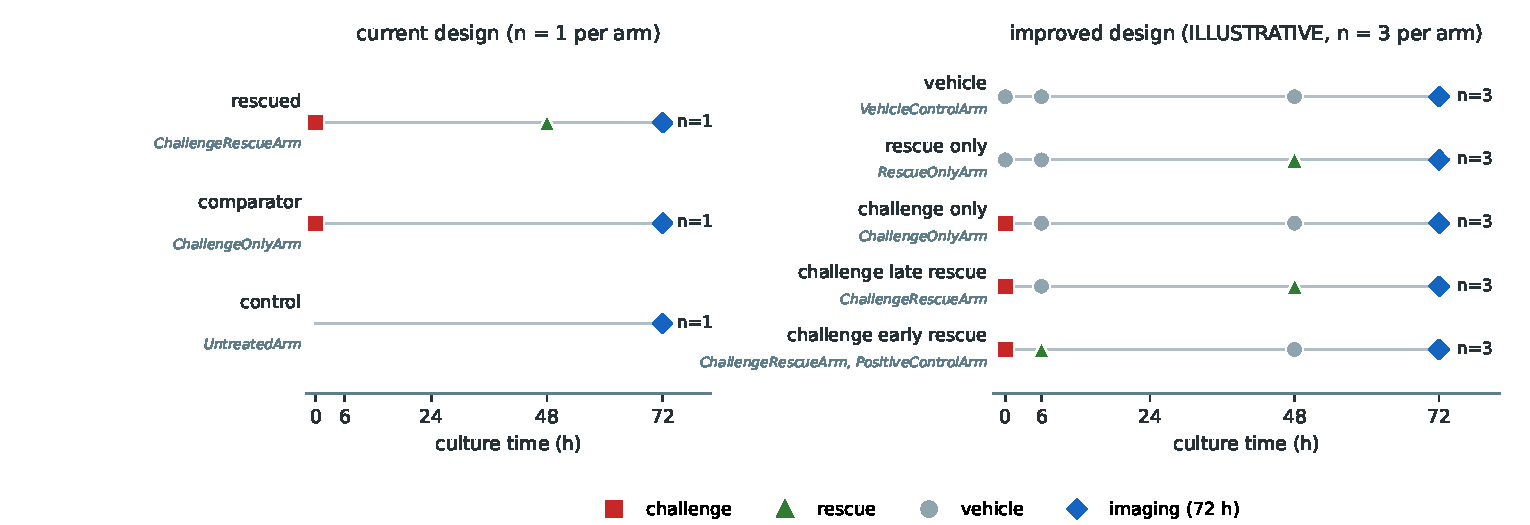
\includegraphics[width=\linewidth,height=0.72\textheight,keepaspectratio]{figures/designs.pdf}
\caption{The two designs on a time axis: administrations of challenge, rescue and vehicle, and imaging at 72~h; under each arm, the classes HermiT infers for it.}\label{fig:designs}\end{figure}


\subsection{An improved design}
The improved design (ILLUSTRATIVE, not run) answers the reviewer: it is a factorial of \emph{challenge} (vehicle,
0.85~au at 0~h) and \emph{time of rescue} (none, 6~h, 48~h), every level vehicle-matched, with 5 of the six
combinations as arms (Table~\ref{tab:imp}). The early-rescue arm is a positive control: its outcome is expected from
prior evidence (rescue at 6~h was effective at every dose tested), so that a null result at 48~h means that the late
rescue fails, not that the agent or the assay failed in this run. Each arm has three units in randomised interior
wells of one plate, and the analysis plan has a rule for each of the 5 comparisons and a deviation rule.
Its expected information gain for the primary contrast is 0.641~bit; the surrogate does not model what the
control arms add.

\begin{table}[tbp]\centering\footnotesize
\caption{Arms of the improved design (ILLUSTRATIVE).}\label{tab:imp}
\begin{tabularx}{\linewidth}{@{}p{3.6cm}p{1.5cm}p{1.7cm}Xp{0.6cm}@{}}\toprule arm & challenge & rescue time & schedule & n \\ \midrule
vehicle & vehicle & none & vehicle 0 au at 0 h; vehicle 0 au at 6 h; vehicle 0 au at 48 h & 3 \\
rescue only & vehicle & h48 & vehicle 0 au at 0 h; vehicle 0 au at 6 h; rescue 0.7 au at 48 h & 3 \\
challenge only & c085 & none & challenge 0.85 au at 0 h; vehicle 0 au at 6 h; vehicle 0 au at 48 h & 3 \\
challenge late rescue & c085 & h48 & challenge 0.85 au at 0 h; vehicle 0 au at 6 h; rescue 0.7 au at 48 h & 3 \\
challenge early rescue & c085 & h6 & challenge 0.85 au at 0 h; rescue 0.7 au at 6 h; vehicle 0 au at 48 h & 3 \\
\bottomrule\end{tabularx}\end{table}

\begin{table}[tbp]\centering\footnotesize
\caption{Comparisons of the improved design.}\label{tab:impcmp}
\begin{tabularx}{\linewidth}{@{}p{2.4cm}Xp{2.0cm}p{1.6cm}p{3.4cm}@{}}\toprule comparison & arms & contrasts & rule & licensed by \\ \midrule
validity & challenge only vs vehicle & challenge & threshold & — \\
primary & challenge late rescue vs challenge only & rescue\_\allowbreak{}time & bayes & validity→primary, positive\_\allowbreak{}control→primary \\
agent\_\allowbreak{}alone & rescue only vs vehicle & rescue\_\allowbreak{}time & estimate & — \\
positive\_\allowbreak{}control & challenge early rescue vs challenge only & rescue\_\allowbreak{}time & threshold & — \\
window & challenge late rescue vs challenge early rescue & rescue\_\allowbreak{}time & estimate & validity→window \\
\bottomrule\end{tabularx}\end{table}

\begin{table}[tbp]\centering\footnotesize
\caption{Realization of the improved design (HermiT).}\label{tab:real2}
\begin{tabularx}{\linewidth}{@{}p{5.0cm}X@{}}\toprule individual & inferred most specific concepts \\ \midrule
\texttt{improved\_\allowbreak{}design} & $\mathsf{AdequatelyControlledInjuryRescueDesign}$, $\mathsf{DeviationAwareDesign}$, $\mathsf{FactorialDesign}$, $\mathsf{HypothesisDiscriminatingDesign}$, $\mathsf{InteractionAwareDesign}$, $\mathsf{RequiresImaging}$, $\mathsf{SufficientlyInformativeDesign}$, $\mathsf{TherapeuticWindowDesign}$ \\
\texttt{improved\_\allowbreak{}objective} & $\mathsf{DiscriminationObjective}$ \\
\texttt{agent\_\allowbreak{}challenge} & $\mathsf{ChallengeAgent}$ \\
\texttt{agent\_\allowbreak{}rescue} & $\mathsf{RescueAgent}$ \\
\texttt{agent\_\allowbreak{}vehicle} & $\mathsf{Vehicle}$ \\
\texttt{improved\_\allowbreak{}arm\_\allowbreak{}vehicle} & $\mathsf{ReplicatedArm}$, $\mathsf{VehicleControlArm}$ \\
\texttt{improved\_\allowbreak{}arm\_\allowbreak{}rescue\_\allowbreak{}only} & $\mathsf{ReplicatedArm}$, $\mathsf{RescueOnlyArm}$ \\
\texttt{improved\_\allowbreak{}arm\_\allowbreak{}challenge\_\allowbreak{}only} & $\mathsf{ChallengeOnlyArm}$, $\mathsf{ReplicatedArm}$ \\
\texttt{improved\_\allowbreak{}arm\_\allowbreak{}challenge\_\allowbreak{}late\_\allowbreak{}rescue} & $\mathsf{ChallengeRescueArm}$, $\mathsf{ReplicatedArm}$ \\
\texttt{improved\_\allowbreak{}arm\_\allowbreak{}challenge\_\allowbreak{}early\_\allowbreak{}rescue} & $\mathsf{ChallengeRescueArm}$, $\mathsf{PositiveControlArm}$, $\mathsf{ReplicatedArm}$ \\
\texttt{improved\_\allowbreak{}cmp\_\allowbreak{}validity} & $\mathsf{CoveredComparison}$, $\mathsf{InjuryValidityComparison}$, $\mathsf{SingleFactorComparison}$ \\
\texttt{improved\_\allowbreak{}cmp\_\allowbreak{}primary} & $\mathsf{CoveredComparison}$, $\mathsf{RescueEffectComparison}$, $\mathsf{SingleFactorComparison}$ \\
\texttt{improved\_\allowbreak{}cmp\_\allowbreak{}agent\_\allowbreak{}alone} & $\mathsf{AgentAloneComparison}$, $\mathsf{CoveredComparison}$, $\mathsf{SingleFactorComparison}$ \\
\texttt{improved\_\allowbreak{}cmp\_\allowbreak{}positive\_\allowbreak{}control} & $\mathsf{CoveredComparison}$, $\mathsf{PositiveControlComparison}$, $\mathsf{RescueEffectComparison}$, $\mathsf{SingleFactorComparison}$ \\
\texttt{improved\_\allowbreak{}cmp\_\allowbreak{}window} & $\mathsf{CoveredComparison}$, $\mathsf{RescueTimingComparison}$, $\mathsf{SingleFactorComparison}$ \\
\bottomrule\end{tabularx}\end{table}


The reasoner classifies the improved design as an \emph{adequately controlled injury--rescue design}, a therapeutic-window
design (two challenge--rescue arms), interaction-aware and deviation-aware (Table~\ref{tab:real2}). The early-rescue
arm is both a challenge--rescue arm and a positive-control arm; the positive-control comparison is also a
rescue-effect comparison, which is correct; and the late-versus-early comparison is a rescue-timing comparison---the
contrast that asks directly whether the rescue's window closes.

\begin{figure}[tbp]\centering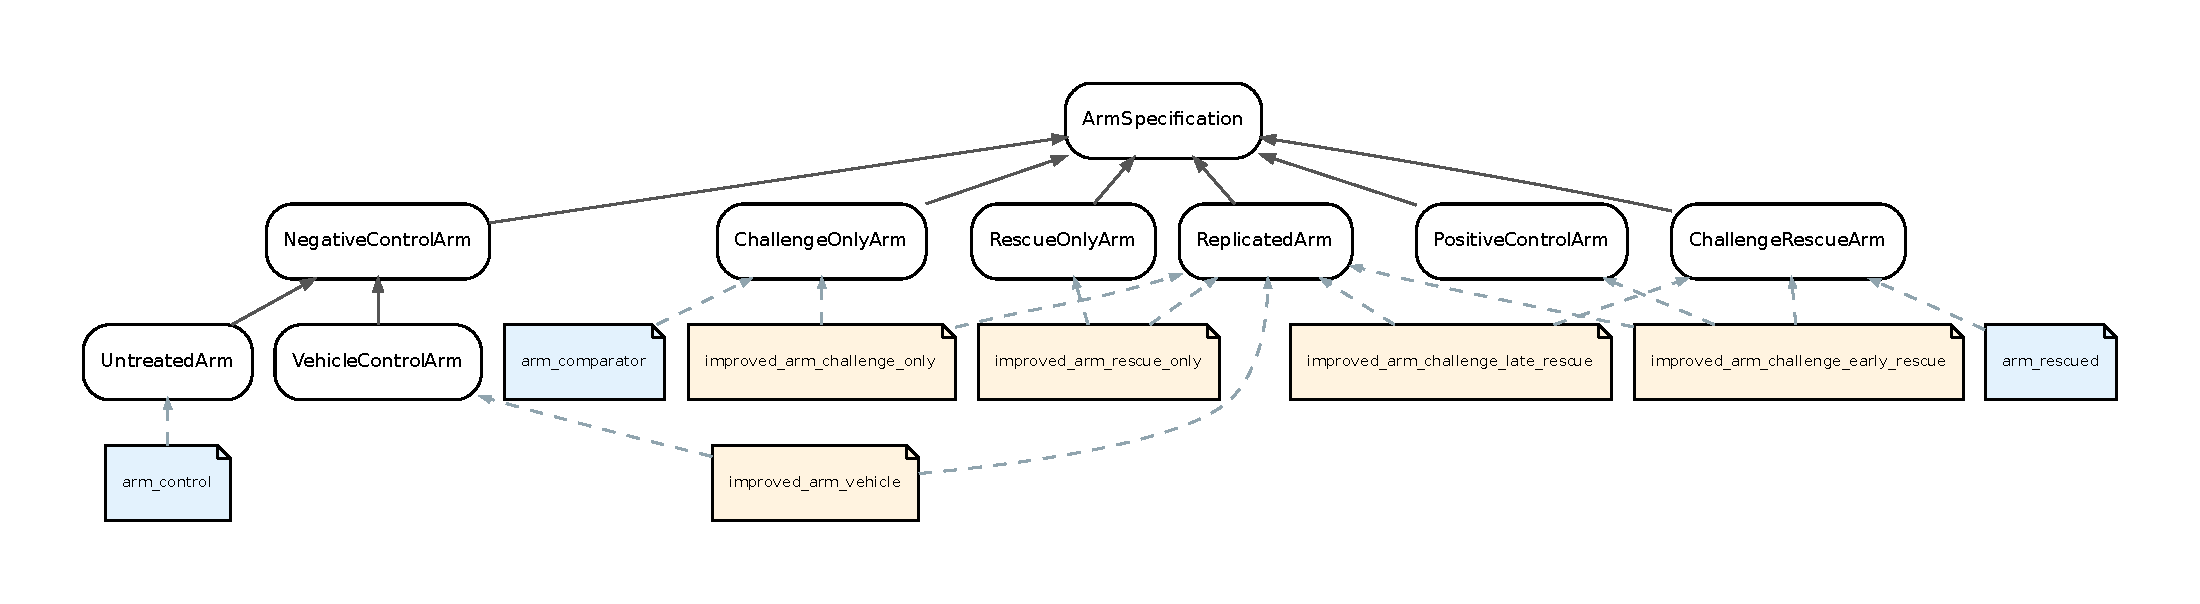
\includegraphics[width=0.92\linewidth,height=0.72\textheight,keepaspectratio]{figures/inferred_arms.pdf}
\caption{Inferred taxonomy of arms, with the arms of the current (blue) and improved (orange) designs realized under it.}\label{fig:infarms}\end{figure}

\begin{figure}[tbp]\centering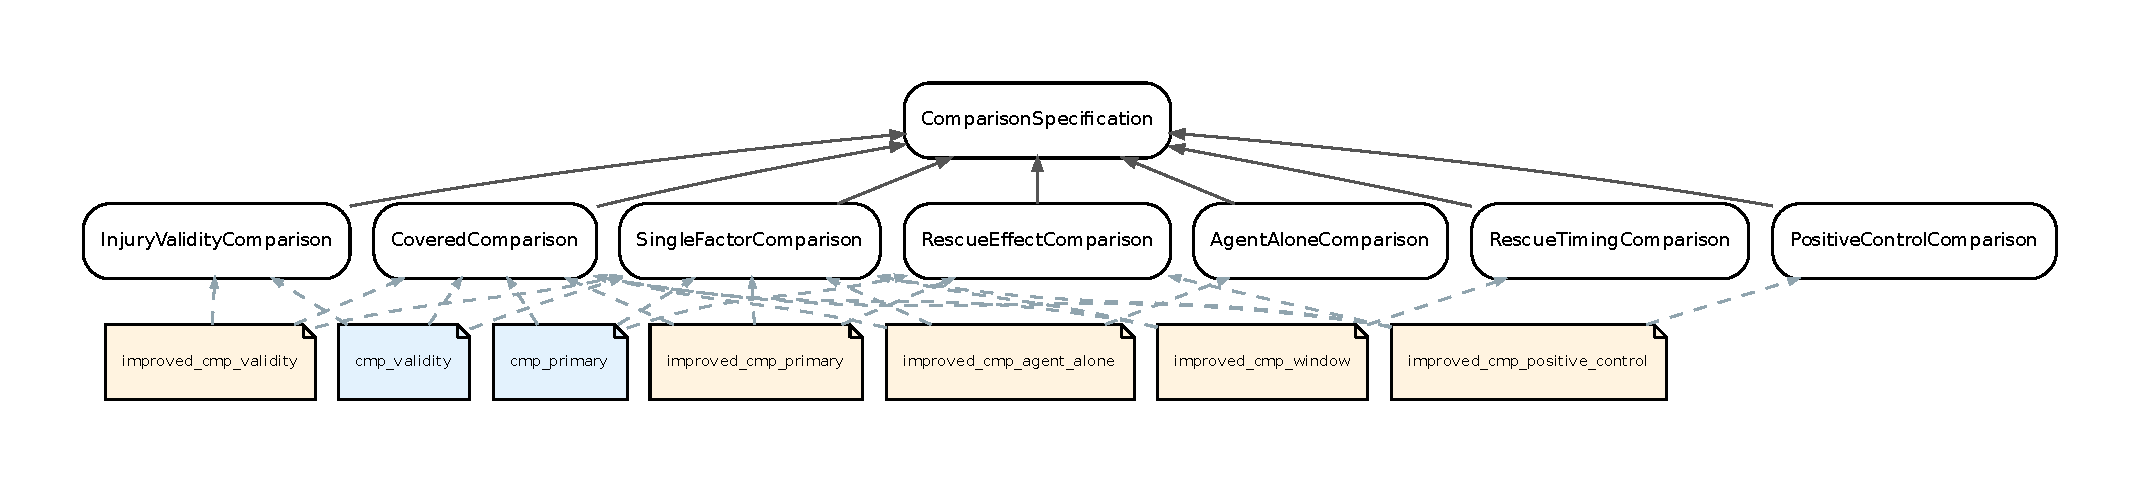
\includegraphics[width=0.92\linewidth,height=0.72\textheight,keepaspectratio]{figures/inferred_comparisons.pdf}
\caption{Inferred taxonomy of comparisons, with both designs' comparisons.}\label{fig:infcmp}\end{figure}

\begin{figure}[tbp]\centering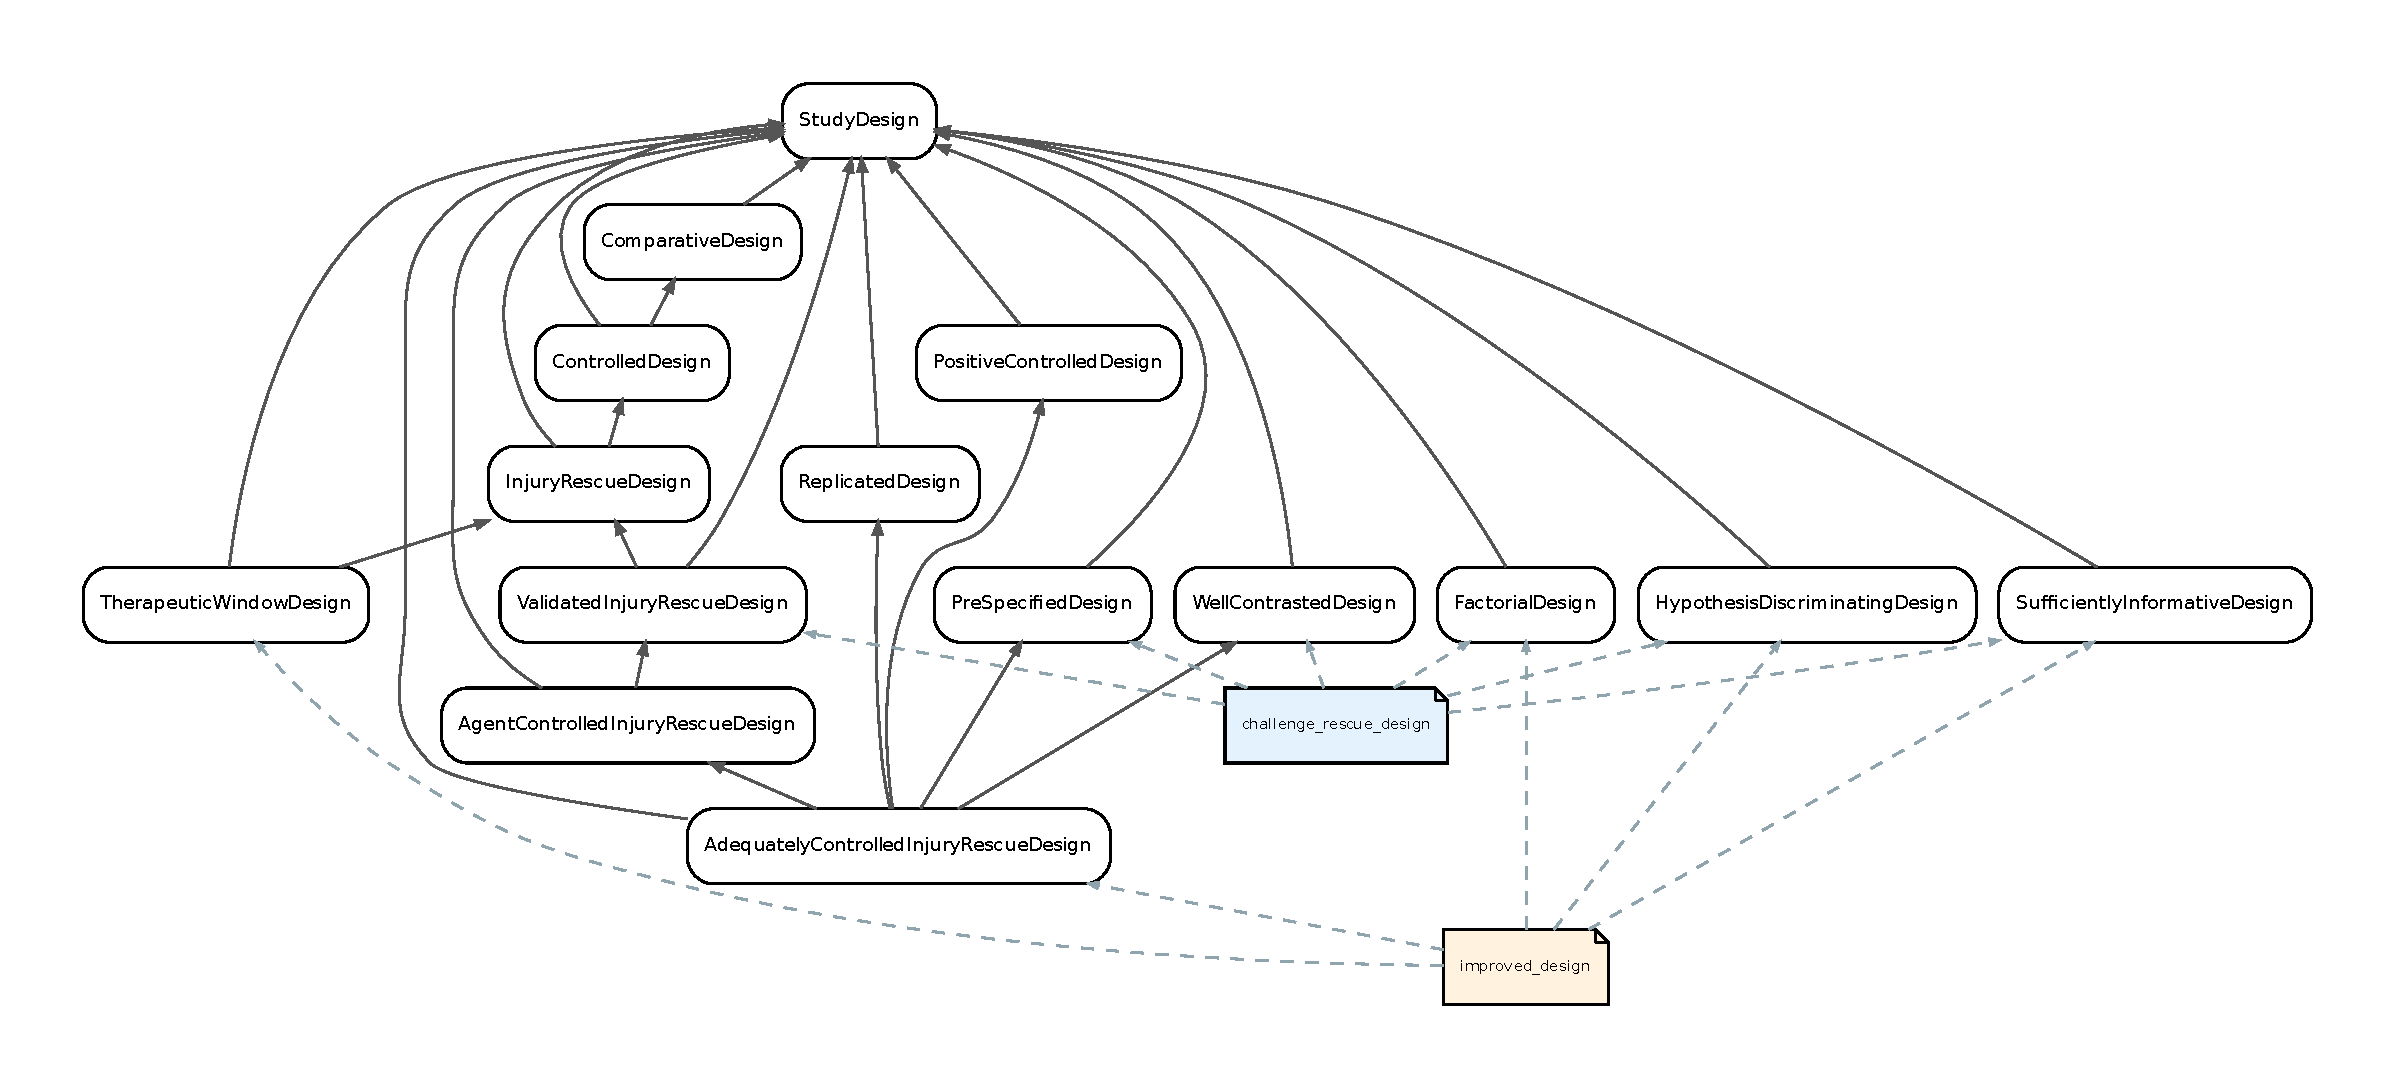
\includegraphics[width=\linewidth,height=0.72\textheight,keepaspectratio]{figures/inferred_designs.pdf}
\caption{Inferred taxonomy of designs, with both designs. Solid edges are subsumptions computed by HermiT; dashed edges are realizations.}\label{fig:infdes}\end{figure}


\subsection{Closed-world checks}
Table~\ref{tab:cw} lists the closed-world checks for both designs. The current design passes the single-factor,
schedule-matching, coverage-by-rules and placement-on-one-plate checks and the execution check, and fails on
interaction estimability (the rescue-only cell is missing), the positive control, replication and edge placement. The
improved design passes every required check; that it is not a full factorial (the vehicle--early-rescue cell is
absent) is reported as information, because no comparison needs that cell.

\begin{table}[tbp]\centering\footnotesize
\caption{Closed-world checks.}\label{tab:cw}
\begin{tabularx}{\linewidth}{@{}p{4.4cm}p{1.2cm}p{1.2cm}X@{}}\toprule check & current & improved & detail (current, else improved) \\ \midrule
every arm has one level of every factor & \textcolor{green!45!black}{pass} & \textcolor{green!45!black}{pass} & 3 arms $\times$ 2 factors \\
single factor: validity & \textcolor{green!45!black}{pass} & \textcolor{green!45!black}{pass} & comparator vs control differ in challenge \\
schedules matched: validity & \textcolor{green!45!black}{pass} & \textcolor{green!45!black}{pass} & administrations differ at 0 h, all belonging to the contrasted factor \\
single factor: primary & \textcolor{green!45!black}{pass} & \textcolor{green!45!black}{pass} & rescued vs comparator differ in rescue \\
schedules matched: primary & \textcolor{green!45!black}{pass} & \textcolor{green!45!black}{pass} & administrations differ at 48 h, all belonging to the contrasted factor \\
full factorial (information, not required) & \textit{info} & \textit{info} & 3 of 4 level combinations; missing: challenge=none, rescue=0p7au\_\allowbreak{}48h \\
interaction estimable & \textcolor{red!65!black}{fail} & \textcolor{green!45!black}{pass} & no complete 2$\times$2 sub-table \\
every comparison has a decision rule & \textcolor{green!45!black}{pass} & \textcolor{green!45!black}{pass} & 2 of 2 \\
positive control licenses the primary comparison & \textcolor{red!65!black}{fail} & \textcolor{green!45!black}{pass} & no positive-control arm \\
replicates $\geq$ 3 per arm & \textcolor{red!65!black}{fail} & \textcolor{green!45!black}{pass} & rescued 1, comparator 1, control 1 \\
units off the plate edge & \textcolor{red!65!black}{fail} & \textcolor{green!45!black}{pass} & edge wells: ['A01', 'A02', 'A05'] \\
all units on one plate & \textcolor{green!45!black}{pass} & \textcolor{green!45!black}{pass} & plate\_\allowbreak{}P17 \\
each administration specification executed once & \textcolor{green!45!black}{pass} & --- & 3 administrations for 3 specifications \\
single factor: agent\_\allowbreak{}alone & --- & \textcolor{green!45!black}{pass} & rescue\_\allowbreak{}only vs vehicle differ in rescue\_\allowbreak{}time \\
schedules matched: agent\_\allowbreak{}alone & --- & \textcolor{green!45!black}{pass} & administrations differ at 48 h, all belonging to the contrasted factor \\
single factor: positive\_\allowbreak{}control & --- & \textcolor{green!45!black}{pass} & challenge\_\allowbreak{}early\_\allowbreak{}rescue vs challenge\_\allowbreak{}only differ in rescue\_\allowbreak{}time \\
schedules matched: positive\_\allowbreak{}control & --- & \textcolor{green!45!black}{pass} & administrations differ at 6 h, all belonging to the contrasted factor \\
single factor: window & --- & \textcolor{green!45!black}{pass} & challenge\_\allowbreak{}late\_\allowbreak{}rescue vs challenge\_\allowbreak{}early\_\allowbreak{}rescue differ in rescue\_\allowbreak{}time \\
schedules matched: window & --- & \textcolor{green!45!black}{pass} & administrations differ at 6 h, 48 h, all belonging to the contrasted factor \\
\bottomrule\end{tabularx}\end{table}


\subsection{Variants}
To check that adequacy is not classified by accident, three variants of the improved design each remove one
ingredient. Each loses exactly the corresponding class and fails exactly the corresponding closed-world check
(Table~\ref{tab:variants}).

\begin{table}[tbp]\centering\footnotesize
\caption{Variants of the improved design.}\label{tab:variants}
\begin{tabularx}{\linewidth}{@{}p{3.8cm}Xp{3.4cm}@{}}\toprule variant & most specific design concepts & closed-world failures \\ \midrule
improved without the positive-control arm & $\mathsf{AgentControlledInjuryRescueDesign}$, $\mathsf{DeviationAwareDesign}$, $\mathsf{FactorialDesign}$, $\mathsf{HypothesisDiscriminatingDesign}$, $\mathsf{InteractionAwareDesign}$, $\mathsf{ReplicatedDesign}$, $\mathsf{RequiresImaging}$, $\mathsf{SufficientlyInformativeDesign}$, $\mathsf{WellContrastedDesign}$ & positive control licenses the primary comparison \\
improved with one unit per arm & $\mathsf{AgentControlledInjuryRescueDesign}$, $\mathsf{DeviationAwareDesign}$, $\mathsf{FactorialDesign}$, $\mathsf{HypothesisDiscriminatingDesign}$, $\mathsf{InteractionAwareDesign}$, $\mathsf{PositiveControlledDesign}$, $\mathsf{RequiresImaging}$, $\mathsf{SufficientlyInformativeDesign}$, $\mathsf{TherapeuticWindowDesign}$, $\mathsf{WellContrastedDesign}$ & replicates $\geq$ 3 per arm \\
improved without a pre-specified analysis & $\mathsf{AgentControlledInjuryRescueDesign}$, $\mathsf{FactorialDesign}$, $\mathsf{HypothesisDiscriminatingDesign}$, $\mathsf{InteractionAwareDesign}$, $\mathsf{PositiveControlledDesign}$, $\mathsf{ReplicatedDesign}$, $\mathsf{RequiresImaging}$, $\mathsf{StudyDesign}$, $\mathsf{SufficientlyInformativeDesign}$, $\mathsf{TherapeuticWindowDesign}$, $\mathsf{WellContrastedDesign}$ & every comparison has a decision rule \\
\bottomrule\end{tabularx}\end{table}


\subsection{Negative controls and inferred subsumptions}
8 modifications must each make the ontology inconsistent; all 8 do (Table~\ref{tab:neg2}). They
exercise kind-preserving parthood, the functionality of assignment, arm closure, the disjointness of what hypotheses
posit, the disjointness of agents, the cardinality of comparison rules, the realization of device functions
(Section~\ref{sec:afford}) and the disjointness of plan parts.

\begin{table}[tbp]\centering\footnotesize
\caption{Negative controls of the OWL axiomatization.}\label{tab:neg2}
\begin{tabularx}{\linewidth}{@{}Xp{4.0cm}@{}}\toprule modification & HermiT \\ \midrule
a well as part of an arm (parthood crosses kinds) & inconsistent, as required \\
a culture assigned to two arms (assignedTo is functional) & inconsistent, as required \\
an administration added to the untreated arm (closure) & inconsistent, as required \\
the graded hypothesis posits a loss of recovery capacity & inconsistent, as required \\
the challenge agent also bears the rescue role (disjoint agents) & inconsistent, as required \\
one decision rule applied to two comparisons & inconsistent, as required \\
an incubation function realized in an imaging assay & inconsistent, as required \\
a factor level that is also an arm (disjoint plan parts) & inconsistent, as required \\
\bottomrule\end{tabularx}\end{table}


The reasoner also derives subsumptions that no axiom states; the 30 found are
$\mathsf{AdequatelyControlledInjuryRescueDesign} \sqsubseteq \mathsf{RequiresDosing}$; $\mathsf{AdequatelyControlledInjuryRescueExperiment} \sqsubseteq \mathsf{ValidatedInjuryRescueExperiment}$; $\mathsf{AgentControlledInjuryRescueDesign} \sqsubseteq \mathsf{RequiresDosing}$; $\mathsf{ComparativeDesign} \sqsubseteq \mathsf{RequiresCultivation}$; $\mathsf{ControlledDesign} \sqsubseteq \mathsf{RequiresCultivation}$; $\mathsf{ControlledExperiment} \sqsubseteq \mathsf{ComparativeExperiment}$; $\mathsf{DeviationAwareDesign} \sqsubseteq \mathsf{RequiresCultivation}$; $\mathsf{FactorialDesign} \sqsubseteq \mathsf{RequiresCultivation}$; $\mathsf{HypothesisDiscriminatingDesign} \sqsubseteq \mathsf{RequiresCultivation}$; $\mathsf{InjuryRescueDesign} \sqsubseteq \mathsf{RequiresDosing}$; $\mathsf{InjuryRescueExperiment} \sqsubseteq \mathsf{ControlledExperiment}$; $\mathsf{InteractionAwareDesign} \sqsubseteq \mathsf{RequiresCultivation}$; $\mathsf{NegativeControlArm} \sqsubseteq \mathsf{ArmSpecification}$; $\mathsf{PositiveControlledDesign} \sqsubseteq \mathsf{RequiresCultivation}$; $\mathsf{PreSpecifiedDesign} \sqsubseteq \mathsf{RequiresCultivation}$; $\mathsf{ReplicatedDesign} \sqsubseteq \mathsf{RequiresCultivation}$; $\mathsf{RequiresAbsorbance} \sqsubseteq \mathsf{RequiresEndpointHandling}$; $\mathsf{RequiresDosing} \sqsubseteq \mathsf{RequiresCultivation}$; $\mathsf{RequiresEndpointHandling} \sqsubseteq \mathsf{RequiresCultivation}$; $\mathsf{RequiresImaging} \sqsubseteq \mathsf{RequiresCultivation}$; $\mathsf{RequiresLuminescence} \sqsubseteq \mathsf{RequiresEndpointHandling}$; $\mathsf{RequiresMultipleEnvironments} \sqsubseteq \mathsf{RequiresCultivation}$; $\mathsf{SufficientlyInformativeDesign} \sqsubseteq \mathsf{RequiresCultivation}$; $\mathsf{TherapeuticWindowDesign} \sqsubseteq \mathsf{RequiresDosing}$; $\mathsf{TherapeuticWindowExperiment} \sqsubseteq \mathsf{InjuryRescueExperiment}$; $\mathsf{UntreatedArm} \sqsubseteq \mathsf{NegativeControlArm}$; $\mathsf{ValidatedInjuryRescueDesign} \sqsubseteq \mathsf{RequiresDosing}$; $\mathsf{ValidatedInjuryRescueExperiment} \sqsubseteq \mathsf{InjuryRescueExperiment}$; $\mathsf{VehicleControlArm} \sqsubseteq \mathsf{NegativeControlArm}$; $\mathsf{WellContrastedDesign} \sqsubseteq \mathsf{RequiresCultivation}$. In particular the whole chain
of experiment classes---adequately controlled, validated, injury--rescue, controlled, comparative---is inferred from
the definitions of the design classes they mirror, and the two negative-control arm classes are recognised as
specializations of their disjunction. The remaining subsumptions place design classes under the requirement classes
of Section~\ref{sec:afford}: whatever has an arm requires cultivation, and every injury--rescue design requires dosing.


\section{What our laboratory affords}\label{sec:afford}
Biomedical laboratories are not general-purpose. What experiments a laboratory affords is fixed by its equipment, the
environments it controls, its containment, the assays it has validated and the reagents it keeps; a cell-culture
laboratory, an imaging core, a plate-reader core and a hypoxia facility afford different experiments, and most
experiments of interest need more than one of them. Cell~01 is a \emph{treatment-and-imaging module}: it incubates,
doses, images, calibrates and quarantines plates, and a clean-sample robot connects it to the rest of the site. A
robot scientist that proposes designs therefore has to know, for each design, whether it can be run here, which of
its steps have to be performed elsewhere, and what is missing. This section adds capability profiles of laboratories
to the ontology, classifies designs by what they require, and matches the two (\texttt{rsa/lab\_\allowbreak{}affordance.py}).

\subsection{Capabilities as device functions}
Following BFO, a capability is modelled as a \emph{function}: a disposition that inheres in a device and is realized
only in processes of one kind. A liquid handler bears a dosing function, realized only in administrations; an imager
bears an imaging function, realized only in imaging assays. A laboratory has its devices as parts, and its capability
classes are \emph{defined} by the functions its devices bear, by the number of controlled environments it provides and
by its validated readout bindings (a binding is information about which quality a device's readout measures, and at
which validation level). The reasoner therefore classifies a laboratory from its devices, and nothing about what a
laboratory can do is asserted directly. Selected axioms:

\ax{\mathsf{Laboratory} ⊑ \mathsf{MaterialEntity} ⊓\allowbreak ∃\mathit{hasDevice}.\mathsf{Device}}
\ax{\mathsf{DeviceFunction} ⊑ \mathsf{Disposition} ⊓\allowbreak ∃\mathit{inheresIn}.\mathsf{Device}}
\ax{\mathsf{DosingFunction} ⊑ \mathsf{DeviceFunction} ⊓\allowbreak ∀\mathit{realizedIn}.\mathsf{Administration}}
\ax{\mathsf{BrightfieldImagingFunction} ⊑ \mathsf{DeviceFunction} ⊓\allowbreak ∀\mathit{realizedIn}.\mathsf{ImagingAssay}}
\ax{\mathsf{DosingLab} ≡ \mathsf{Laboratory} ⊓\allowbreak ∃\mathit{hasDevice}.∃\mathit{bearerOf}.\mathsf{DosingFunction}}
\ax{\mathsf{MultiEnvironmentLab} ≡ \mathsf{Laboratory} ⊓\allowbreak (≥2 \mathit{providesEnvironment}.\mathsf{EnvironmentProfile})}
\ax{\mathsf{ValidatedSizeReadoutLab} ≡ \mathsf{Laboratory} ⊓\allowbreak ∃\mathit{hasReadoutBinding}.(\mathsf{ValidatedReadoutBinding} ⊓\allowbreak ∃\mathit{isAbout}.\mathsf{OrganoidSize})}
\ax{\mathsf{TreatmentAndImagingModule} ≡ \mathsf{DosingLab} ⊓\allowbreak \mathsf{CultivationLab} ⊓\allowbreak \mathsf{BrightfieldImagingLab} ⊓\allowbreak \mathsf{ValidatedSizeReadoutLab}}

Reagent stocks are located in a laboratory (\textit{stocks}), not parts of it, and an environment profile is a plan
specification that a laboratory realizes, so that two incubators running at the same setpoints count as one
environment. Because a function is realized only in processes of its kind, a function realized in the wrong kind of
process is a contradiction: an incubation function realized in an imaging assay is the eighth negative control of
Table~\ref{tab:neg2}.

\subsection{Design requirements}
What a design needs from a laboratory follows from its content, so requirement classes are defined as well: a design
with an administration requires dosing, one with an imaging readout requires imaging, one with an endpoint readout
(luminescence, absorbance) requires the corresponding reader and endpoint handling, and one with an environment factor
requires as many controlled environments as the factor has levels.

\ax{\mathsf{RequiresDosing} ≡ \mathsf{StudyDesign} ⊓\allowbreak ∃\mathit{hasArm}.∃\mathit{hasAdministrationSpec}.\mathsf{AdministrationSpecification}}
\ax{\mathsf{RequiresImaging} ≡ \mathsf{StudyDesign} ⊓\allowbreak ∃\mathit{hasReadout}.\mathsf{ImagingReadout}}
\ax{\mathsf{RequiresLuminescence} ≡ \mathsf{StudyDesign} ⊓\allowbreak ∃\mathit{hasReadout}.\mathsf{LuminescenceReadout}}
\ax{\mathsf{RequiresEndpointHandling} ≡ \mathsf{StudyDesign} ⊓\allowbreak ∃\mathit{hasReadout}.\mathsf{EndpointReadout}}
\ax{\mathsf{RequiresMultipleEnvironments} ≡ \mathsf{StudyDesign} ⊓\allowbreak ∃\mathit{hasFactor}.\mathsf{EnvironmentFactor}}

Each requirement is met by one capability class (Table~\ref{tab:reqcap}). This correspondence is a table, not an
axiom: it relates classes of different categories (designs and laboratories), and stating it as a subsumption would
make every design a laboratory. The reasoner adds requirements no axiom states for a design class: every injury--rescue
design, validated or adequately controlled, requires dosing; every design that has an arm requires cultivation; and
luminescence and absorbance readouts require endpoint handling (Section~\ref{sec:results}).

\begin{table}[tbp]\centering\footnotesize
\caption{Requirements and the capabilities that meet them.}\label{tab:reqcap}
\begin{tabularx}{\linewidth}{@{}XX@{}}\toprule design requirement & met by laboratory capability \\ \midrule
$\mathsf{RequiresDosing}$ & $\mathsf{DosingLab}$ \\
$\mathsf{RequiresCultivation}$ & $\mathsf{CultivationLab}$ \\
$\mathsf{RequiresImaging}$ & $\mathsf{BrightfieldImagingLab}$ \\
$\mathsf{RequiresLuminescence}$ & $\mathsf{LuminescenceReadoutLab}$ \\
$\mathsf{RequiresAbsorbance}$ & $\mathsf{AbsorbanceReadoutLab}$ \\
$\mathsf{RequiresMultipleEnvironments}$ & $\mathsf{MultiEnvironmentLab}$ \\
\bottomrule\end{tabularx}\end{table}


\subsection{Cell~01's profile}
Cell~01's profile is not written by hand; it is read from three sources in the repository. The ten component records
list each device's capability verbs, which a table maps to device functions (Table~\ref{tab:c01dev}); the device
registry lists the reagent stocks and the readout bindings with their validation level; and the twin's measured
durations give the time a dosing session takes. Verbs without a function (aspirate, autofocus, press a button) are
steps of the functions' realizations, not capabilities of their own, and are not mapped.

\begin{table}[tbp]\centering\footnotesize
\caption{Cell~01's devices, their capability verbs and the functions they are evidence of.}\label{tab:c01dev}
\begin{tabularx}{\linewidth}{@{}>{\raggedright\arraybackslash}p{4.0cm}>{\raggedright\arraybackslash}X>{\raggedright\arraybackslash}p{3.6cm}@{}}\toprule device (component record) & capability verbs & functions \\ \midrule
H4 Quarantine Station & isolate\_\allowbreak{}sample, retain\_\allowbreak{}invalid\_\allowbreak{}run, prevent\_\allowbreak{}reentry, release\_\allowbreak{}by\_\allowbreak{}authorization & QuarantineFunction \\
L09 Automated Plate Hotel & buffer\_\allowbreak{}plate, store\_\allowbreak{}plate, retrieve\_\allowbreak{}plate, report\_\allowbreak{}inventory, reserve\_\allowbreak{}slot, verify\_\allowbreak{}identity & StorageFunction \\
L10 Automated CO2 Incubator & incubate\_\allowbreak{}plate, maintain\_\allowbreak{}environment, store\_\allowbreak{}plate, release\_\allowbreak{}plate, report\_\allowbreak{}environment, raise\_\allowbreak{}excursion\_\allowbreak{}alarm & IncubationFunction, StorageFunction \\
L12 Automated Liquid-Handling Station & pick\_\allowbreak{}tip, detect\_\allowbreak{}liquid\_\allowbreak{}surface, aspirate, dispense, mix, dose\_\allowbreak{}well, eject\_\allowbreak{}tip & DosingFunction \\
L17 Bright-Field Imaging Station & load\_\allowbreak{}plate, autofocus, image\_\allowbreak{}well, image\_\allowbreak{}plate\_\allowbreak{}region, compute\_\allowbreak{}focus\_\allowbreak{}quality, export\_\allowbreak{}raw\_\allowbreak{}image & BrightfieldImagingFunction \\
L21 Quality-Control and Calibration Station & run\_\allowbreak{}reference\_\allowbreak{}measurement, validate\_\allowbreak{}imager, validate\_\allowbreak{}barcode, validate\_\allowbreak{}tool\_\allowbreak{}frame & CalibrationFunction \\
R01 Fixed Precision Plate-Handling Arm & pick\_\allowbreak{}sbs\_\allowbreak{}plate, place\_\allowbreak{}sbs\_\allowbreak{}plate, handover\_\allowbreak{}plate, reseat\_\allowbreak{}plate, inspect\_\allowbreak{}grasp, move\_\allowbreak{}plate\_\allowbreak{}between\_\allowbreak{}local\_\allowbreak{}stations & PlateHandlingFunction \\
R02 Rail-Mounted Flexible Manipulation System & translate\_\allowbreak{}workspace, pick\_\allowbreak{}plate, pick\_\allowbreak{}tube, handle\_\allowbreak{}rack, press\_\allowbreak{}button, turn\_\allowbreak{}selector, open\_\allowbreak{}access\_\allowbreak{}door, change\_\allowbreak{}tool, inspect\_\allowbreak{}station & --- \\
R03 Clean Sample AMR with H2 Deterministic Dock & navigate, transport\_\allowbreak{}clean\_\allowbreak{}sample, dock\_\allowbreak{}precisely, handover\_\allowbreak{}carrier, opportunity\_\allowbreak{}charge & TransportFunction \\
R02 Automatic Tool Changer and Tool Magazine & dock\_\allowbreak{}tool, lock\_\allowbreak{}tool, verify\_\allowbreak{}tool, unlock\_\allowbreak{}tool, store\_\allowbreak{}tool, select\_\allowbreak{}tool\_\allowbreak{}for\_\allowbreak{}task & --- \\
\bottomrule\end{tabularx}\end{table}


Cell~01 provides one controlled environment (37\,\textdegree C, 5\,\% CO$_2$,
90\,\% humidity, from the incubator's record), stocks the agents challenge, rescue,
and has one validated readout binding: the imaging station's organoid radius, a readout of organoid size. A plate may
be outside the incubator for at most 600~s per excursion; a dosing session costs about 205~s of
transfers (two legs of each robot arm, retrieval, storage, tool coupling) and 35.6~s per well, so at most
\textbf{11 wells} can be dosed per session (these durations are the twin's, ILLUSTRATIVE).

HermiT classifies the laboratories in 1.76~s, with both laboratories and all four designs in one ontology
(Table~\ref{tab:labcaps}). Cell~01 is a treatment-and-imaging module; it is not an endpoint-reader, metabolic-readout
or multi-environment laboratory, because it has no endpoint reader, no validated metabolic readout and one
environment. A second laboratory, a site core facility with a multimode plate reader and a dock for the clean-sample
robot, is ILLUSTRATIVE (not modelled from records); it stands in for the facilities to which steps that Cell~01
cannot perform are allocated.

\begin{table}[tbp]\centering\footnotesize
\caption{Capability classes of the two laboratories (HermiT).}\label{tab:labcaps}
\begin{tabularx}{\linewidth}{@{}>{\raggedright\arraybackslash}p{3.2cm}>{\raggedright\arraybackslash}X>{\raggedright\arraybackslash}X@{}}\toprule laboratory & is (HermiT) & is not \\ \midrule
Cell 01 (automated treatment-and-imaging module) & $\mathsf{BrightfieldImagingLab}$, $\mathsf{ConnectedLab}$, $\mathsf{ContainmentCapableLab}$, $\mathsf{CultivationLab}$, $\mathsf{DosingLab}$, $\mathsf{QualityControlledLab}$, $\mathsf{TreatmentAndImagingModule}$, $\mathsf{ValidatedSizeReadoutLab}$ & $\mathsf{AbsorbanceReadoutLab}$, $\mathsf{LuminescenceReadoutLab}$, $\mathsf{MultiEnvironmentLab}$, $\mathsf{ValidatedMetabolicReadoutLab}$ \\
Core facility: multimode plate reader (ILLUSTRATIVE) & $\mathsf{AbsorbanceReadoutLab}$, $\mathsf{ConnectedLab}$, $\mathsf{LuminescenceReadoutLab}$, $\mathsf{ValidatedMetabolicReadoutLab}$ & $\mathsf{BrightfieldImagingLab}$, $\mathsf{ContainmentCapableLab}$, $\mathsf{CultivationLab}$, $\mathsf{DosingLab}$, $\mathsf{MultiEnvironmentLab}$, $\mathsf{QualityControlledLab}$, $\mathsf{TreatmentAndImagingModule}$, $\mathsf{ValidatedSizeReadoutLab}$ \\
\bottomrule\end{tabularx}\end{table}


\subsection{Matching designs against laboratories}
Whether a design is executable is a closed-world question over the individuals: it concerns the laboratories and
stocks the site has, not those it might have. For each design, the matcher (i) takes the requirement classes HermiT
infers for it and allocates each to a laboratory with the meeting capability, Cell~01 first; (ii) checks that every
agent the design administers is stocked where the dosing happens; (iii) checks that each readout has a validated
binding to the quality it is about in the allocated laboratory; (iv) counts the environments an environment factor
needs; (v) splits the doses due at each time point into sessions that fit the excursion window; (vi) checks the units
against the 60 interior wells of one plate; (vii) checks that destructive endpoint readouts come
after every imaging; and (viii) checks that a transfer to every other allocated laboratory is possible (both
connected). The verdict is \emph{executable in Cell~01}, \emph{executable on site with transfers}, or \emph{not
executable as modelled} with what is missing; when only reagents are missing, the matcher also reports the verdict
with them stocked.

\begin{table}[tbp]\centering\footnotesize
\caption{What Cell~01 and the site afford: four designs (ILLUSTRATIVE).}\label{tab:afford}
\begin{tabularx}{\linewidth}{@{}>{\raggedright\arraybackslash}p{3.6cm}>{\raggedright\arraybackslash}p{2.8cm}>{\raggedright\arraybackslash}p{2.0cm}>{\raggedright\arraybackslash}X>{\raggedright\arraybackslash}p{2.2cm}@{}}\toprule design & requires (HermiT) & verdict & missing & with reagents stocked \\ \midrule
the current challenge-rescue design & Cultivation, Dosing, Imaging & executable in Cell 01 & --- & --- \\
the improved design (vehicle, rescue-only, early rescue, 3 replicates) & Cultivation, Dosing, Imaging & not executable as modelled & reagent not stocked in Cell 01: vehicle & executable in Cell 01 \\
the improved design with an ATP luminescence endpoint at 72 h & Cultivation, Dosing, EndpointHandling, Imaging, Luminescence & not executable as modelled & reagent not stocked in Cell 01: vehicle & executable on site with transfers \\
a challenge x oxygen design (environment factor) & Cultivation, Dosing, Imaging, MultipleEnvironments & not executable as modelled & RequiresMultipleEnvironments: no laboratory is a MultiEnvironmentLab & --- \\
\bottomrule\end{tabularx}\end{table}

\begin{figure}[tbp]\centering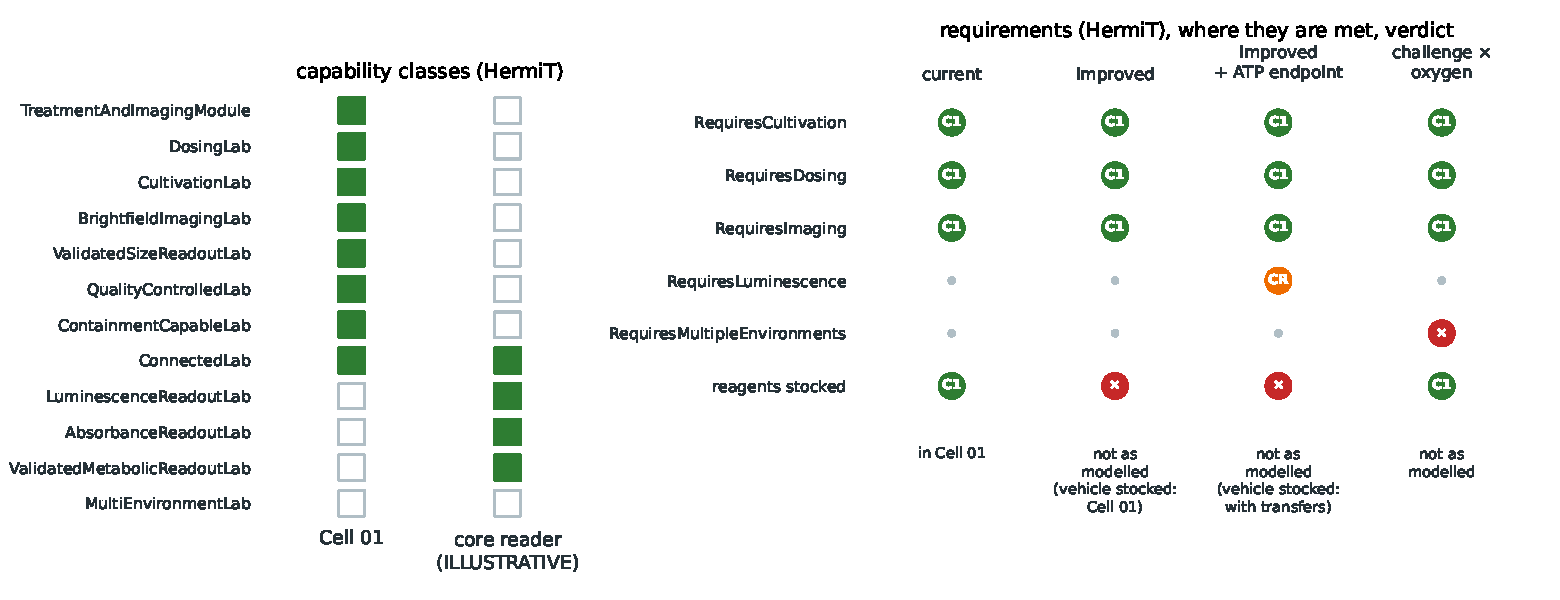
\includegraphics[width=\linewidth,height=0.72\textheight,keepaspectratio]{figures/affordance.pdf}
\caption{Left: capability classes HermiT infers for the two laboratories. Right: the requirements of the four designs and the laboratory each is allocated to (C1 Cell~01, CR core reader, $\times$ unmet), with the verdict below.}\label{fig:afford}\end{figure}


\subsection{Four designs}
\paragraph{The current design} requires cultivation, dosing and imaging, all met by Cell~01, with both agents
stocked and a validated size readout; its three doses (two at 0~h, one at 48~h) take one session each. It is
\emph{executable in Cell 01}.

\paragraph{The improved design} has the same requirements, but administers a vehicle that Cell~01 does not stock, so
it is \emph{not executable as modelled}; with the vehicle stocked it would be
\emph{executable in Cell 01}. Its 15 units receive 15
administrations at each of 0, 6 and 48~h, more than the 11 that fit one excursion, so each time point needs two
sessions and the last wells are dosed about ten minutes after the first. Against a rescue delay of 6 or 48~h this is
small, but it is systematic if the arms are dosed in a fixed order; the sessions should interleave the arms, which is
the same randomisation that the placement check asks for on the plate.

\paragraph{The improved design with an ATP endpoint} adds a luminescence readout of metabolic activity at 72~h,
after the imaging. HermiT classifies it as requiring luminescence and endpoint handling, which no device of Cell~01
offers; the step is allocated to the core reader, which has a validated binding for it, and the transfer is possible
because both laboratories are connected by the clean-sample robot. With the vehicle stocked it is \emph{executable on
site with transfers}. The time the plate spends outside the controlled environment on the way is not modelled; since
the ATP read is the last step and destructive, it does not affect the imaging readout.

\paragraph{The challenge $\times$ oxygen design} varies the environment (normoxia, hypoxia) as a factor. It requires
4 capabilities, among them $\mathsf{MultiEnvironmentLab}$: two controlled
environments, of which Cell~01 provides one and the core facility none. It is \emph{not executable as modelled};
running it would need a second incubator at a different oxygen setpoint, or a hypoxia facility and transfers.

\subsection{What the scope is, and what it is not}
Within the modelled designs, Cell~01 affords in-vitro experiments on cultures in one plate, in one environment, with
treatments by the agents it stocks and imaging of organoid size as the readout: injury, rescue and agent-control
designs, therapeutic-window designs and their factorials, up to 11 administrations per session and
60 interior wells per plate. It affords designs with endpoint assays only together with a core
facility, and designs with environment factors not at all. For the adequately controlled design of
Section~\ref{sec:results} the only missing resource is a vehicle stock.

Three limitations bound this result. The map from capability verbs to functions is hand-written, and the general
manipulation verbs of the rail-mounted robot are not mapped, so capabilities that need a tool change are not
represented. The core facility, the vehicle and the durations are ILLUSTRATIVE, and transfer times between
laboratories are not modelled. And what can be dosed, imaged or read is classified, but whether an assay is suitable
for a question (sensitivity, dynamic range) is not: that is a property of a validated binding, which is recorded as a
level and not reasoned about.


\section{Relation to existing standards}\label{sec:related}
Table~\ref{tab:std} relates the framework to existing standards. None of them combines the three things the robot
scientist needs: a design layer with comparisons and controls defined by purpose, a reasoner that classifies designs
from their content, and a link to the plans the robot executes. OBI is the closest in spirit and would be the natural
upper ontology to import; the reporting guidelines list many of the criteria that the closed-world layer checks, but
for human authors and after the fact.

\begin{table}[tbp]\centering\footnotesize
\caption{Existing standards and the framework.}\label{tab:std}
\begin{tabularx}{\linewidth}{@{}p{3.0cm}Xp{1.8cm}XX@{}}\toprule standard & covers & layers & used here as & gap \\ \midrule
ISA \citep{sansone2012} & investigation, study, assay; factors and factor values per sample & design, data & units, factors, assays & no comparisons, controls by purpose, adequacy, reasoning \\
OBI \citep{bandrowski2016} & planned processes, study designs, assays, roles; BFO & all five & the style of the upper level, roles, assays & this work adds defined design classes and adequacy \\
EXPO \citep{soldatova2006} & investigations, hypotheses, designs, results & epistemic, design & hypothesis--design--result link & no defined control or comparison types \\
CDISC SDM \citep{cdisc_sdm} & arms, epochs, cells, activities (clinical) & design & arms $\times$ epochs = our arms $\times$ phases & clinical only; no logic \\
EXACT \citep{soldatova2008}, LabOP, Autoprotocol & protocol steps, parameters, containers & protocol, execution & our lab designators and CRAM plans & no design layer \\
ARRIVE \citep{kilkenny2010}, CONSORT \citep{schulz2010} & reporting checklists & design (reported) & replication, randomisation, blinding, controls & checked by humans after the fact \\
\bottomrule\end{tabularx}\end{table}


\section{Discussion}\label{sec:discussion}
\paragraph{What the representation buys.} The final representation turns a reviewer's judgement into a computation
before the experiment is run. That the current design lacks agent and positive controls and replication is not a
comment in a report but the absence of a class in a realization; that the improved design has them is a derived fact
with a proof (the reasoner's), not an assertion. The same machinery explains a design: the classes an arm or a
comparison belongs to say what it is for. And because the actions and their order are derived from the design, a
change of design---a new arm, a new comparison---changes the plan the robot executes without hand editing.

\paragraph{Open and closed world.} The division of labour between OWL and the closed-world queries is not a
workaround but a consequence of the questions asked. ``What kind of design is this?'' is a question about what follows
from what is stated, which the open world answers soundly once the design's own extent is closed. ``Does this design
contain three replicates per arm?'' is a question about the design as given, which only the closed world answers.
Making the closure explicit in the ABox, rather than switching to closed-world semantics wholesale, keeps the
classification monotonic: adding an arm can only add classes.

\paragraph{Defined versus primitive concepts.} The LDL concept layer checked an experiment against the concept it
declared; the OWL layer \emph{finds} the concepts an experiment belongs to. The difference matters for a robot
scientist that generates designs: it should not need to know in advance what kind of experiment it has produced.

\paragraph{The proxy and the posit.} Two modelling decisions carry the D016 discipline into the ontology. Data are
proxies: the size datum is about organoid size and a proxy for viability; that viability is what the experiment is
about is visible, and so is the assumption. Hypotheses posit: the threshold hypothesis posits a loss of recovery
capacity; the graded one is defined by not positing it, and a graded hypothesis that posits it is inconsistent. The
ontology can thus represent competing biology without committing to any of it.

\paragraph{The case study as a test.} The case is small, but it exercises every layer: an epistemic objective with
an information target, a design with comparisons of different purposes, a protocol refined into lab actions, an
execution with an audit trail, and a hidden biological state reached through a proxy. The reviewer's critique of
Section~\ref{sec:case} served as an independent specification of what the representation should detect, and it does.


\section{Limitations}\label{sec:limits}
\begin{itemize}
\item \textbf{Not executed.} The CRAM/RPL plans are generated and checked but not executed; no Lisp CRAM is installed.
  The surrogate run is a simulation, and its numbers are ILLUSTRATIVE (D016).
\item \textbf{Two layers not yet joined.} Factors, levels, positive controls and the analysis plan exist in the OWL
  layer; the authored \texttt{experiment.ldl}, the LDL concept checker and the CRAM plans do not have them yet. The
  current design's factors are read off its schedules.
\item \textbf{Upper ontology in style only.} BFO and OBI are followed in style, in an own namespace, not imported;
  the alignment to Cell~01's biology ontology is by subsumption where the meaning is the same.
\item \textbf{Illustrative criteria.} The minimum of three replicates, the 0.5~bit information target and the
  validity criterion (an effect below zero by more than two standard deviations) are placeholders, not recommendations.
\item \textbf{Coverage.} The taxonomy covers in-vitro injury--rescue experiments. Positive controls are defined;
  randomisation is checked only as placement off the plate edge; blinding, blocking, technical versus biological
  replicates, dose--response and time-course designs, and the in vivo and clinical branches are not axiomatized.
\item \textbf{Information of control arms.} The information-gain model covers the primary contrast; it does not
  represent what control arms add (the confounds they exclude are outside the surrogate).
\item \textbf{Laboratory profiles.} Capability verbs are mapped to device functions by a hand-written table; the
  rail-mounted robot's general manipulation is not mapped; the core facility, the vehicle and the durations are
  ILLUSTRATIVE; transfer times between laboratories, assay suitability and costs are not modelled.
\item \textbf{Reproducibility pipeline.} The generators of this report are not yet stages of \texttt{rsa.reproduce};
  adding them would change the manifest hash quoted by the companion report and paper.
\item \textbf{References.} The references were compiled without database access and must be checked before
  publication.
\end{itemize}


\section{Roadmap}\label{sec:roadmap}
\begin{enumerate}
\item \textbf{One source.} Extend \texttt{experiment.ldl} with factors, levels, readouts and the analysis plan; generate
  the OWL ABox, the culture plan and the CRAM plans from it, so that every layer derives from one authored design.
\item \textbf{Adequacy in the loop.} Make the reasoner's classification a constraint of the design planner: among the
  designs that reach the information target, choose the cheapest \emph{adequately controlled} one, and report the
  classes a cheaper design would lose.
\item \textbf{Affordance in the loop.} Restrict the design planner to designs the site affords, and report for
  each rejected design what resource would make it executable (a stock, a reader, an environment).
\item \textbf{Information of controls.} Extend the surrogate and the information-gain model with the confounds the
  control arms exclude (agent effects, vehicle effects, plate position), so that their value is quantified.
\item \textbf{Import the upper ontology.} Replace the BFO-style upper level by BFO and OBI imports, and align the design
  classes with OBI's study-design terms.
\item \textbf{Broaden the taxonomy.} Add blinding, blocking, replicate kinds, dose--response and time-course designs,
  and the in vivo and clinical branches (arms $\times$ epochs).
\item \textbf{Shapes.} Express the closed-world checks as SHACL shapes over the reasoned ABox, so that they are
  portable beyond the RSA.
\item \textbf{Reproducibility.} Add the generators to \texttt{rsa.reproduce} and record the ontology, ABox and reasoner
  results in the manifest.
\end{enumerate}

\FloatBarrier
\bibliographystyle{unsrtnat}
\bibliography{refs}
\appendix
\section{The TBox in DL notation}\label{app:tbox}
The complete TBox as generated from \texttt{rsa/experiment\_\allowbreak{}ontology.py}. Concepts are set in $\mathsf{sans}$, roles in $\mathit{italics}$.
\subsection*{Upper level}{\small A BFO-style upper level. Continuants (material entities, qualities, realizable entities, information content entities) and occurrents (processes) are disjoint; planned processes are distinct from biological processes.}
{\small\begin{multicols}{2}
\ax{\mathsf{MaterialEntity} ⊑ \mathsf{Continuant}}
\ax{\mathsf{SpecificallyDependentContinuant} ⊑ \mathsf{Continuant}}
\ax{\mathsf{Quality} ⊑ \mathsf{SpecificallyDependentContinuant}}
\ax{\mathsf{RealizableEntity} ⊑ \mathsf{SpecificallyDependentContinuant}}
\ax{\mathsf{InformationContentEntity} ⊑ \mathsf{Continuant}}
\ax{\mathsf{Process} ⊑ \mathsf{Occurrent}}
\ax{\mathsf{Continuant} ⊓\allowbreak \mathsf{Occurrent} ⊑ ⊥}
\ax{\mathrm{Disjoint}(\mathsf{MaterialEntity},\allowbreak \mathsf{SpecificallyDependentContinuant},\allowbreak \mathsf{InformationContentEntity})}
\ax{\mathsf{Quality} ⊓\allowbreak \mathsf{RealizableEntity} ⊑ ⊥}
\ax{\mathsf{Role} ⊑ \mathsf{RealizableEntity}}
\ax{\mathsf{Disposition} ⊑ \mathsf{RealizableEntity}}
\ax{\mathsf{Role} ⊓\allowbreak \mathsf{Disposition} ⊑ ⊥}
\ax{\mathsf{PlannedProcess} ⊑ \mathsf{Process}}
\ax{\mathsf{BiologicalProcess} ⊑ \mathsf{Process}}
\ax{\mathsf{PlannedProcess} ⊓\allowbreak \mathsf{BiologicalProcess} ⊑ ⊥}
\ax{\mathsf{PlanSpecification} ⊑ \mathsf{InformationContentEntity}}
\ax{\mathsf{DataItem} ⊑ \mathsf{InformationContentEntity}}
\ax{\mathsf{Hypothesis} ⊑ \mathsf{InformationContentEntity}}
\ax{\mathsf{Objective} ⊑ \mathsf{InformationContentEntity}}
\ax{\mathsf{Conclusion} ⊑ \mathsf{InformationContentEntity}}
\ax{\mathrm{Disjoint}(\mathsf{PlanSpecification},\allowbreak \mathsf{DataItem},\allowbreak \mathsf{Hypothesis},\allowbreak \mathsf{Objective},\allowbreak \mathsf{Conclusion})}
\end{multicols}}
\subsection*{Relations and partonomy}{\small Parthood is transitive and kind-preserving: processes have processes as parts, material entities material entities, information entities information entities. Its kinds are simple sub-roles (so they may be counted). Location, membership, participation, execution and bearing are not parthood.}
{\small\begin{multicols}{2}
\ax{\mathrm{Trans}(\mathit{hasPart})}
\ax{\mathit{partOf} ≡ \mathit{hasPart}^{-}}
\ax{\mathit{hasPhase} ⊑ \mathit{hasPart}}
\ax{\mathit{hasStep} ⊑ \mathit{hasPart}}
\ax{\mathit{hasWell} ⊑ \mathit{hasPart}}
\ax{\mathit{hasOrganoid} ⊑ \mathit{hasPart}}
\ax{\mathit{hasCell} ⊑ \mathit{hasPart}}
\ax{\mathit{hasMedium} ⊑ \mathit{hasPart}}
\ax{\mathit{hasArm} ⊑ \mathit{hasPart}}
\ax{\mathit{hasComparisonSpec} ⊑ \mathit{hasPart}}
\ax{\mathit{hasAdministrationSpec} ⊑ \mathit{hasPart}}
\ax{\mathit{hasObjective} ⊑ \mathit{hasPart}}
\ax{\mathsf{Process} ⊑ ∀\mathit{hasPart}.\mathsf{Process}}
\ax{\mathsf{MaterialEntity} ⊑ ∀\mathit{hasPart}.\mathsf{MaterialEntity}}
\ax{\mathsf{InformationContentEntity} ⊑ ∀\mathit{hasPart}.\mathsf{InformationContentEntity}}
\ax{\mathit{containedIn} ≡ \mathit{contains}^{-}}
\ax{\mathit{containedIn} ∘ \mathit{partOf} ⊑ \mathit{locatedIn}}
\ax{\mathit{participatesIn} ≡ \mathit{hasParticipant}^{-}}
\ax{\mathit{hasPart} ∘ \mathit{hasParticipant} ⊑ \mathit{hasParticipant}}
\ax{\mathit{hasSpecifiedInput} ⊑ \mathit{hasParticipant}}
\ax{\mathit{inheresIn} ≡ \mathit{bearerOf}^{-}}
\ax{\mathrm{Func}(\mathit{inheresIn})}
\ax{\mathit{hasAssignedUnit} ≡ \mathit{assignedTo}^{-}}
\ax{\mathrm{Func}(\mathit{assignedTo})}
\ax{\mathrm{Func}(\mathit{usesAgent})}
\ax{\mathrm{Trans}(\mathit{precedes})}
\ax{∃\mathit{executes}.⊤ ⊑ \mathsf{PlannedProcess}}
\ax{⊤ ⊑ ∀\mathit{executes}.\mathsf{PlanSpecification}}
\ax{∃\mathit{isAbout}.⊤ ⊑ \mathsf{InformationContentEntity}}
\ax{∃\mathit{bearerOf}.⊤ ⊑ \mathsf{Continuant}}
\ax{⊤ ⊑ ∀\mathit{bearerOf}.\mathsf{SpecificallyDependentContinuant}}
\ax{∃\mathit{realizedIn}.⊤ ⊑ \mathsf{RealizableEntity}}
\ax{⊤ ⊑ ∀\mathit{realizedIn}.\mathsf{Process}}
\ax{\mathrm{Func}(\mathit{dose_au})}
\ax{\mathrm{Func}(\mathit{atTime_h})}
\ax{\mathrm{Func}(\mathit{fromTime_h})}
\ax{\mathrm{Func}(\mathit{toTime_h})}
\ax{\mathrm{Func}(\mathit{expectedInformationGain_bits})}
\ax{\mathrm{Func}(\mathit{radius_um})}
\ax{\mathrm{Func}(\mathit{wellRow})}
\ax{\mathrm{Func}(\mathit{wellColumn})}
\end{multicols}}
\subsection*{Biological material and labware}{\small An organoid culture is organoids in medium; an organoid has cells. A well holds at most one culture; a culture is in a well, not part of it. Chemical agents bear roles in the experiment (challenge, rescue, vehicle) and dispositions (toxicity); size is a quality of organoids, viability and recovery capacity are dispositions of cultures.}
{\small
\ax{\mathsf{OrganoidCulture} ⊑ \mathsf{MaterialEntity} ⊓\allowbreak ∃\mathit{hasOrganoid}.\mathsf{Organoid} ⊓\allowbreak ∃\mathit{hasMedium}.\mathsf{CultureMedium}}
\ax{\mathsf{Organoid} ⊑ \mathsf{MaterialEntity} ⊓\allowbreak ∃\mathit{hasCell}.\mathsf{Cell}}
\ax{\mathsf{Cell} ⊑ \mathsf{MaterialEntity}}
\ax{\mathsf{CultureMedium} ⊑ \mathsf{MaterialEntity}}
\ax{\mathsf{ChemicalAgent} ⊑ \mathsf{MaterialEntity}}
\ax{\mathsf{Plate} ⊑ \mathsf{MaterialEntity} ⊓\allowbreak ∃\mathit{hasWell}.\mathsf{Well}}
\ax{\mathsf{Well} ⊑ \mathsf{MaterialEntity} ⊓\allowbreak (≤1 \mathit{contains}.\mathsf{OrganoidCulture})}
\ax{\mathrm{Disjoint}(\mathsf{OrganoidCulture},\allowbreak \mathsf{Organoid},\allowbreak \mathsf{Cell},\allowbreak \mathsf{CultureMedium},\allowbreak \mathsf{ChemicalAgent},\allowbreak \mathsf{Plate},\allowbreak \mathsf{Well})}
\ax{\mathsf{OrganoidSize} ⊑ \mathsf{Quality} ⊓\allowbreak ∃\mathit{inheresIn}.\mathsf{Organoid}}
\ax{\mathsf{Viability} ⊑ \mathsf{Disposition} ⊓\allowbreak ∃\mathit{inheresIn}.\mathsf{OrganoidCulture} ⊓\allowbreak ∀\mathit{realizedIn}.\mathsf{CultureGrowth}}
\ax{\mathsf{RecoveryCapacity} ⊑ \mathsf{Disposition} ⊓\allowbreak ∃\mathit{inheresIn}.\mathsf{OrganoidCulture} ⊓\allowbreak ∀\mathit{realizedIn}.\mathsf{RecoveryProcess}}
\ax{\mathsf{ToxicityDisposition} ⊑ \mathsf{Disposition} ⊓\allowbreak ∃\mathit{inheresIn}.\mathsf{ChemicalAgent} ⊓\allowbreak ∀\mathit{realizedIn}.\mathsf{InjuryProcess}}
\ax{\mathsf{Toxicant} ≡ \mathsf{ChemicalAgent} ⊓\allowbreak ∃\mathit{bearerOf}.\mathsf{ToxicityDisposition}}
\ax{\mathsf{ChallengeAgentRole} ⊑ \mathsf{Role}}
\ax{\mathsf{RescueAgentRole} ⊑ \mathsf{Role}}
\ax{\mathsf{VehicleRole} ⊑ \mathsf{Role}}
\ax{\mathsf{ExperimentalUnitRole} ⊑ \mathsf{Role}}
\ax{\mathrm{Disjoint}(\mathsf{ChallengeAgentRole},\allowbreak \mathsf{RescueAgentRole},\allowbreak \mathsf{VehicleRole},\allowbreak \mathsf{ExperimentalUnitRole})}
\ax{\mathsf{ChallengeAgent} ≡ \mathsf{ChemicalAgent} ⊓\allowbreak ∃\mathit{bearerOf}.\mathsf{ChallengeAgentRole}}
\ax{\mathsf{RescueAgent} ≡ \mathsf{ChemicalAgent} ⊓\allowbreak ∃\mathit{bearerOf}.\mathsf{RescueAgentRole}}
\ax{\mathsf{Vehicle} ≡ \mathsf{ChemicalAgent} ⊓\allowbreak ∃\mathit{bearerOf}.\mathsf{VehicleRole}}
\ax{\mathrm{Disjoint}(\mathsf{ChallengeAgent},\allowbreak \mathsf{RescueAgent},\allowbreak \mathsf{Vehicle})}
\ax{\mathsf{ChallengeAgent} ⊑ \mathsf{Toxicant}}
\ax{\mathsf{ExperimentalUnit} ≡ \mathsf{OrganoidCulture} ⊓\allowbreak ∃\mathit{bearerOf}.\mathsf{ExperimentalUnitRole}}
}
\subsection*{Biological processes}{\small Processes in which the cultures participate. A loss of recovery capacity (a point of no return) is a process type that hypotheses may posit; nothing here asserts that it occurs.}
{\small
\ax{\mathsf{InjuryProcess} ⊑ \mathsf{BiologicalProcess} ⊓\allowbreak ∃\mathit{hasParticipant}.\mathsf{OrganoidCulture}}
\ax{\mathsf{ProtectiveResponse} ⊑ \mathsf{BiologicalProcess} ⊓\allowbreak ∃\mathit{hasParticipant}.\mathsf{OrganoidCulture}}
\ax{\mathsf{RecoveryProcess} ⊑ \mathsf{BiologicalProcess} ⊓\allowbreak ∃\mathit{hasParticipant}.\mathsf{OrganoidCulture}}
\ax{\mathsf{CellDeath} ⊑ \mathsf{BiologicalProcess} ⊓\allowbreak ∃\mathit{hasParticipant}.\mathsf{OrganoidCulture}}
\ax{\mathsf{CultureGrowth} ⊑ \mathsf{BiologicalProcess} ⊓\allowbreak ∃\mathit{hasParticipant}.\mathsf{OrganoidCulture}}
\ax{\mathsf{LossOfRecoveryCapacity} ⊑ \mathsf{BiologicalProcess} ⊓\allowbreak ∃\mathit{hasParticipant}.\mathsf{OrganoidCulture}}
\ax{\mathrm{Disjoint}(\mathsf{InjuryProcess},\allowbreak \mathsf{ProtectiveResponse},\allowbreak \mathsf{RecoveryProcess},\allowbreak \mathsf{CellDeath},\allowbreak \mathsf{CultureGrowth})}
}
\subsection*{Plans: designs, arms, administrations, comparisons}{\small A study design has arms and comparisons; an arm specifies the administrations its units receive (agent, dose, time). Arm types are defined by what is administered, comparison types by the arms compared, design types by their arms and comparisons; the reasoner classifies them. Replication and the information target are ILLUSTRATIVE design criteria.}
{\small
\ax{\mathsf{StudyDesign} ⊑ \mathsf{PlanSpecification} ⊓\allowbreak ∃\mathit{hasObjective}.\mathsf{Objective} ⊓\allowbreak ∃\mathit{hasArm}.\mathsf{ArmSpecification}}
\ax{\mathsf{ArmSpecification} ⊑ \mathsf{PlanSpecification} ⊓\allowbreak ∀\mathit{hasAdministrationSpec}.\mathsf{AdministrationSpecification}}
\ax{\mathsf{AdministrationSpecification} ⊑ \mathsf{PlanSpecification} ⊓\allowbreak (=1 \mathit{usesAgent}.\mathsf{ChemicalAgent}) ⊓\allowbreak ∃\mathit{dose_au}.\mathsf{decimal} ⊓\allowbreak ∃\mathit{atTime_h}.\mathsf{decimal}}
\ax{\mathsf{ComparisonSpecification} ⊑ \mathsf{PlanSpecification} ⊓\allowbreak (=2 \mathit{compares}.\mathsf{ArmSpecification})}
\ax{\mathrm{Disjoint}(\mathsf{StudyDesign},\allowbreak \mathsf{ArmSpecification},\allowbreak \mathsf{AdministrationSpecification},\allowbreak \mathsf{ComparisonSpecification})}
\ax{\mathsf{ChallengeSpec} ≡ \mathsf{AdministrationSpecification} ⊓\allowbreak ∃\mathit{usesAgent}.\mathsf{ChallengeAgent}}
\ax{\mathsf{RescueSpec} ≡ \mathsf{AdministrationSpecification} ⊓\allowbreak ∃\mathit{usesAgent}.\mathsf{RescueAgent}}
\ax{\mathsf{VehicleSpec} ≡ \mathsf{AdministrationSpecification} ⊓\allowbreak ∃\mathit{usesAgent}.\mathsf{Vehicle}}
\ax{\mathsf{UntreatedArm} ≡ \mathsf{ArmSpecification} ⊓\allowbreak ¬∃\mathit{hasAdministrationSpec}.\mathsf{AdministrationSpecification}}
\ax{\mathsf{VehicleControlArm} ≡ \mathsf{ArmSpecification} ⊓\allowbreak ∃\mathit{hasAdministrationSpec}.\mathsf{VehicleSpec} ⊓\allowbreak ¬∃\mathit{hasAdministrationSpec}.(\mathsf{ChallengeSpec} ⊔\allowbreak \mathsf{RescueSpec})}
\ax{\mathsf{NegativeControlArm} ≡ \mathsf{UntreatedArm} ⊔\allowbreak \mathsf{VehicleControlArm}}
\ax{\mathsf{ChallengeOnlyArm} ≡ \mathsf{ArmSpecification} ⊓\allowbreak ∃\mathit{hasAdministrationSpec}.\mathsf{ChallengeSpec} ⊓\allowbreak ¬∃\mathit{hasAdministrationSpec}.\mathsf{RescueSpec}}
\ax{\mathsf{RescueOnlyArm} ≡ \mathsf{ArmSpecification} ⊓\allowbreak ∃\mathit{hasAdministrationSpec}.\mathsf{RescueSpec} ⊓\allowbreak ¬∃\mathit{hasAdministrationSpec}.\mathsf{ChallengeSpec}}
\ax{\mathsf{ChallengeRescueArm} ≡ \mathsf{ArmSpecification} ⊓\allowbreak ∃\mathit{hasAdministrationSpec}.\mathsf{ChallengeSpec} ⊓\allowbreak ∃\mathit{hasAdministrationSpec}.\mathsf{RescueSpec}}
\ax{\mathsf{ReplicatedArm} ≡ \mathsf{ArmSpecification} ⊓\allowbreak (≥3 \mathit{hasAssignedUnit}.\mathsf{ExperimentalUnit})}
\ax{\mathsf{InjuryValidityComparison} ≡ \mathsf{ComparisonSpecification} ⊓\allowbreak ∃\mathit{compares}.\mathsf{ChallengeOnlyArm} ⊓\allowbreak ∃\mathit{compares}.\mathsf{NegativeControlArm}}
\ax{\mathsf{RescueEffectComparison} ≡ \mathsf{ComparisonSpecification} ⊓\allowbreak ∃\mathit{compares}.\mathsf{ChallengeRescueArm} ⊓\allowbreak ∃\mathit{compares}.\mathsf{ChallengeOnlyArm}}
\ax{\mathsf{AgentAloneComparison} ≡ \mathsf{ComparisonSpecification} ⊓\allowbreak ∃\mathit{compares}.\mathsf{RescueOnlyArm} ⊓\allowbreak ∃\mathit{compares}.\mathsf{NegativeControlArm}}
\ax{\mathsf{RescueTimingComparison} ≡ \mathsf{ComparisonSpecification} ⊓\allowbreak (=2 \mathit{compares}.\mathsf{ChallengeRescueArm})}
\ax{\mathsf{DiscriminationObjective} ≡ \mathsf{Objective} ⊓\allowbreak (≥2 \mathit{isAbout}.\mathsf{Hypothesis})}
}
\subsection*{Factors, levels and treatments}{\small A factor is what the experimenter varies (here: the challenge, the time of the rescue); its levels are the values it takes, each specifying administrations. An arm's treatment is one level of every factor (atLevel; a level is shared by arms, so this is not parthood). A comparison contrasts the factors in which its two arms differ; a well-formed comparison contrasts exactly one. Which factors a comparison contrasts, and whether an arm's schedule is the union of its levels, are computed under the closed world and asserted.}
{\small
\ax{\mathsf{Factor} ⊑ \mathsf{PlanSpecification} ⊓\allowbreak (≥2 \mathit{hasLevel}.\mathsf{FactorLevel})}
\ax{\mathsf{FactorLevel} ⊑ \mathsf{PlanSpecification} ⊓\allowbreak (=1 \mathit{levelOf}.\mathsf{Factor})}
\ax{\mathit{levelOf} ≡ \mathit{hasLevel}^{-}}
\ax{\mathit{hasLevel} ⊑ \mathit{hasPart}}
\ax{\mathit{hasFactor} ⊑ \mathit{hasPart}}
\ax{\mathsf{ArmSpecification} ⊑ ∀\mathit{atLevel}.\mathsf{FactorLevel}}
\ax{\mathsf{ComparisonSpecification} ⊑ ∀\mathit{contrasts}.\mathsf{Factor}}
\ax{\mathsf{SingleFactorComparison} ≡ \mathsf{ComparisonSpecification} ⊓\allowbreak (=1 \mathit{contrasts}.\mathsf{Factor})}
\ax{\mathsf{FactorialDesign} ≡ \mathsf{StudyDesign} ⊓\allowbreak (≥2 \mathit{hasFactor}.\mathsf{Factor})}
\ax{\mathsf{WellContrastedDesign} ≡ \mathsf{StudyDesign} ⊓\allowbreak ∀\mathit{hasComparisonSpec}.\mathsf{SingleFactorComparison}}
\ax{\mathsf{InteractionContrast} ⊑ \mathsf{PlanSpecification} ⊓\allowbreak (=2 \mathit{differenceOf}.\mathsf{ComparisonSpecification})}
\ax{\mathit{hasInteractionContrast} ⊑ \mathit{hasPart}}
\ax{\mathsf{InteractionAwareDesign} ≡ \mathsf{StudyDesign} ⊓\allowbreak ∃\mathit{hasInteractionContrast}.\mathsf{InteractionContrast}}
\ax{\mathrm{Disjoint}(\mathsf{Factor},\allowbreak \mathsf{FactorLevel},\allowbreak \mathsf{StudyDesign},\allowbreak \mathsf{ArmSpecification},\allowbreak \mathsf{AdministrationSpecification},\allowbreak \mathsf{ComparisonSpecification},\allowbreak \mathsf{InteractionContrast})}
}
\subsection*{Controls}{\small A control is defined by what it controls for. Negative controls (untreated, vehicle) give the baseline; the agent-alone arm separates the rescue agent's own effect from rescue of injury; a positive control is an arm whose outcome is expected from prior evidence, so that a null result elsewhere can be interpreted (the agent and the assay worked in this run).}
{\small
\ax{\mathsf{Expectation} ⊑ \mathsf{DataItem}}
\ax{\mathsf{PriorEvidence} ⊑ \mathsf{DataItem}}
\ax{\mathsf{EvidenceBasedExpectation} ≡ \mathsf{Expectation} ⊓\allowbreak ∃\mathit{derivedFrom}.\mathsf{PriorEvidence}}
\ax{\mathsf{PositiveControlArm} ≡ \mathsf{ArmSpecification} ⊓\allowbreak ∃\mathit{hasExpectedOutcome}.\mathsf{EvidenceBasedExpectation}}
\ax{\mathsf{PositiveControlComparison} ≡ \mathsf{ComparisonSpecification} ⊓\allowbreak ∃\mathit{compares}.\mathsf{PositiveControlArm} ⊓\allowbreak ∃\mathit{compares}.\mathsf{ChallengeOnlyArm}}
\ax{\mathsf{PositiveControlledDesign} ≡ \mathsf{StudyDesign} ⊓\allowbreak ∃\mathit{hasComparisonSpec}.\mathsf{PositiveControlComparison}}
}
\subsection*{Readouts and analysis plan}{\small A readout (endpoint) specifies what is measured, when and by which assay, and what it is a proxy for. The analysis plan, part of the design and fixed before the run, has one decision rule per comparison (a threshold test, a Bayesian update over the hypotheses, or an estimate) and a rule for deviations. A design is pre-specified when every comparison is covered by a rule.}
{\small
\ax{\mathit{hasReadout} ⊑ \mathit{hasPart}}
\ax{\mathit{hasAnalysisPlan} ⊑ \mathit{hasPart}}
\ax{\mathit{hasDecisionRule} ⊑ \mathit{hasPart}}
\ax{\mathsf{ReadoutSpecification} ⊑ \mathsf{PlanSpecification} ⊓\allowbreak ∃\mathit{measures}.\mathsf{Quality} ⊓\allowbreak ∃\mathit{atTime_h}.\mathsf{decimal}}
\ax{\mathsf{SizeReadout} ≡ \mathsf{ReadoutSpecification} ⊓\allowbreak ∃\mathit{measures}.\mathsf{OrganoidSize} ⊓\allowbreak ∃\mathit{isProxyFor}.\mathsf{Viability}}
\ax{\mathsf{AnalysisPlan} ⊑ \mathsf{PlanSpecification} ⊓\allowbreak ∃\mathit{hasDecisionRule}.\mathsf{DecisionRule}}
\ax{\mathsf{DecisionRule} ⊑ \mathsf{PlanSpecification}}
\ax{\mathsf{ComparisonRule} ⊑ \mathsf{DecisionRule} ⊓\allowbreak (=1 \mathit{appliesTo}.\mathsf{ComparisonSpecification})}
\ax{\mathsf{ThresholdRule} ⊑ \mathsf{ComparisonRule}}
\ax{\mathsf{EstimationRule} ⊑ \mathsf{ComparisonRule}}
\ax{\mathsf{BayesianUpdateRule} ⊑ \mathsf{ComparisonRule} ⊓\allowbreak (≥2 \mathit{isAbout}.\mathsf{Hypothesis})}
\ax{\mathsf{DeviationRule} ⊑ \mathsf{DecisionRule} ⊓\allowbreak ¬∃\mathit{appliesTo}.⊤}
\ax{\mathrm{Disjoint}(\mathsf{ThresholdRule},\allowbreak \mathsf{EstimationRule},\allowbreak \mathsf{BayesianUpdateRule},\allowbreak \mathsf{DeviationRule})}
\ax{\mathrm{Disjoint}(\mathsf{ReadoutSpecification},\allowbreak \mathsf{AnalysisPlan},\allowbreak \mathsf{DecisionRule},\allowbreak \mathsf{Factor},\allowbreak \mathsf{StudyDesign},\allowbreak \mathsf{ArmSpecification},\allowbreak \mathsf{ComparisonSpecification})}
\ax{\mathsf{CoveredComparison} ≡ \mathsf{ComparisonSpecification} ⊓\allowbreak ∃\mathit{appliesTo}^{-}.\mathsf{ComparisonRule}}
\ax{\mathsf{PreSpecifiedDesign} ≡ \mathsf{StudyDesign} ⊓\allowbreak ∃\mathit{hasReadout}.\mathsf{ReadoutSpecification} ⊓\allowbreak ∃\mathit{hasAnalysisPlan}.\mathsf{AnalysisPlan} ⊓\allowbreak ∀\mathit{hasComparisonSpec}.\mathsf{CoveredComparison}}
\ax{\mathsf{DeviationAwareDesign} ≡ \mathsf{PreSpecifiedDesign} ⊓\allowbreak ∃\mathit{hasAnalysisPlan}.∃\mathit{hasDecisionRule}.\mathsf{DeviationRule}}
}
\subsection*{Design classes}{\small Design types are defined by their arms, comparisons, factors and analysis plan; the reasoner places every design under each class it satisfies. Adequate control (the reviewer's standard) requires the agent-alone and vehicle controls, a positive control, replication, single-factor comparisons and a pre-specified analysis. Replication and the information target are ILLUSTRATIVE criteria.}
{\small
\ax{\mathsf{ComparativeDesign} ≡ \mathsf{StudyDesign} ⊓\allowbreak (≥2 \mathit{hasArm}.\mathsf{ArmSpecification}) ⊓\allowbreak ∃\mathit{hasComparisonSpec}.\mathsf{ComparisonSpecification}}
\ax{\mathsf{ControlledDesign} ≡ \mathsf{ComparativeDesign} ⊓\allowbreak ∃\mathit{hasArm}.\mathsf{NegativeControlArm}}
\ax{\mathsf{InjuryRescueDesign} ≡ \mathsf{ControlledDesign} ⊓\allowbreak ∃\mathit{hasArm}.\mathsf{ChallengeRescueArm} ⊓\allowbreak ∃\mathit{hasArm}.\mathsf{ChallengeOnlyArm} ⊓\allowbreak ∃\mathit{hasComparisonSpec}.\mathsf{RescueEffectComparison}}
\ax{\mathsf{ValidatedInjuryRescueDesign} ≡ \mathsf{InjuryRescueDesign} ⊓\allowbreak ∃\mathit{hasComparisonSpec}.\mathsf{InjuryValidityComparison}}
\ax{\mathsf{AgentControlledInjuryRescueDesign} ≡ \mathsf{ValidatedInjuryRescueDesign} ⊓\allowbreak ∃\mathit{hasArm}.\mathsf{RescueOnlyArm} ⊓\allowbreak ∃\mathit{hasArm}.\mathsf{VehicleControlArm} ⊓\allowbreak ∃\mathit{hasComparisonSpec}.\mathsf{AgentAloneComparison}}
\ax{\mathsf{TherapeuticWindowDesign} ≡ \mathsf{InjuryRescueDesign} ⊓\allowbreak (≥2 \mathit{hasArm}.\mathsf{ChallengeRescueArm})}
\ax{\mathsf{ReplicatedDesign} ≡ \mathsf{StudyDesign} ⊓\allowbreak ∀\mathit{hasArm}.\mathsf{ReplicatedArm}}
\ax{\mathsf{AdequatelyControlledInjuryRescueDesign} ≡ \mathsf{AgentControlledInjuryRescueDesign} ⊓\allowbreak \mathsf{PositiveControlledDesign} ⊓\allowbreak \mathsf{ReplicatedDesign} ⊓\allowbreak \mathsf{WellContrastedDesign} ⊓\allowbreak \mathsf{PreSpecifiedDesign}}
\ax{\mathsf{HypothesisDiscriminatingDesign} ≡ \mathsf{StudyDesign} ⊓\allowbreak ∃\mathit{hasObjective}.\mathsf{DiscriminationObjective}}
\ax{\mathsf{SufficientlyInformativeDesign} ≡ \mathsf{StudyDesign} ⊓\allowbreak ∃\mathit{expectedInformationGain_bits}.\mathsf{decimal}_{\geq 0.5}}
}
\subsection*{Experiments, phases and steps}{\small An experiment (investigation) is a planned process that executes exactly one study design; its classification follows its design's. Its parts are three phases, their parts the steps: administrations and incubations, assays, data transformations.}
{\small
\ax{\mathsf{Investigation} ⊑ \mathsf{PlannedProcess} ⊓\allowbreak (=1 \mathit{executes}.\mathsf{StudyDesign})}
\ax{\mathsf{ComparativeExperiment} ≡ \mathsf{Investigation} ⊓\allowbreak ∃\mathit{executes}.\mathsf{ComparativeDesign}}
\ax{\mathsf{ControlledExperiment} ≡ \mathsf{Investigation} ⊓\allowbreak ∃\mathit{executes}.\mathsf{ControlledDesign}}
\ax{\mathsf{InjuryRescueExperiment} ≡ \mathsf{Investigation} ⊓\allowbreak ∃\mathit{executes}.\mathsf{InjuryRescueDesign}}
\ax{\mathsf{ValidatedInjuryRescueExperiment} ≡ \mathsf{Investigation} ⊓\allowbreak ∃\mathit{executes}.\mathsf{ValidatedInjuryRescueDesign}}
\ax{\mathsf{AdequatelyControlledInjuryRescueExperiment} ≡ \mathsf{Investigation} ⊓\allowbreak ∃\mathit{executes}.\mathsf{AdequatelyControlledInjuryRescueDesign}}
\ax{\mathsf{TherapeuticWindowExperiment} ≡ \mathsf{Investigation} ⊓\allowbreak ∃\mathit{executes}.\mathsf{TherapeuticWindowDesign}}
\ax{\mathsf{FactorialExperiment} ≡ \mathsf{Investigation} ⊓\allowbreak ∃\mathit{executes}.\mathsf{FactorialDesign}}
\ax{\mathsf{HypothesisDiscriminatingExperiment} ≡ \mathsf{Investigation} ⊓\allowbreak ∃\mathit{executes}.\mathsf{HypothesisDiscriminatingDesign}}
\ax{\mathsf{ComparativeExperiment} ⊑ (=1 \mathit{hasPhase}.\mathsf{CultivationPhase}) ⊓\allowbreak (=1 \mathit{hasPhase}.\mathsf{ObservationPhase}) ⊓\allowbreak (=1 \mathit{hasPhase}.\mathsf{AnalysisPhase})}
\ax{\mathsf{Phase} ⊑ \mathsf{PlannedProcess}}
\ax{\mathsf{CultivationPhase} ⊑ \mathsf{Phase} ⊓\allowbreak ∀\mathit{hasStep}.(\mathsf{Administration} ⊔\allowbreak \mathsf{Incubation})}
\ax{\mathsf{ObservationPhase} ⊑ \mathsf{Phase} ⊓\allowbreak ∀\mathit{hasStep}.\mathsf{Assay}}
\ax{\mathsf{AnalysisPhase} ⊑ \mathsf{Phase} ⊓\allowbreak ∀\mathit{hasStep}.\mathsf{DataTransformation}}
\ax{\mathrm{Disjoint}(\mathsf{CultivationPhase},\allowbreak \mathsf{ObservationPhase},\allowbreak \mathsf{AnalysisPhase})}
\ax{\mathsf{Administration} ⊑ \mathsf{PlannedProcess} ⊓\allowbreak (=1 \mathit{executes}.\mathsf{AdministrationSpecification}) ⊓\allowbreak ∃\mathit{hasSpecifiedInput}.\mathsf{ChemicalAgent} ⊓\allowbreak ∃\mathit{hasSpecifiedInput}.\mathsf{ExperimentalUnit}}
\ax{\mathsf{ChallengeAdministration} ≡ \mathsf{Administration} ⊓\allowbreak ∃\mathit{executes}.\mathsf{ChallengeSpec}}
\ax{\mathsf{RescueAdministration} ≡ \mathsf{Administration} ⊓\allowbreak ∃\mathit{executes}.\mathsf{RescueSpec}}
\ax{\mathsf{Incubation} ⊑ \mathsf{PlannedProcess} ⊓\allowbreak ∃\mathit{hasParticipant}.\mathsf{OrganoidCulture}}
\ax{\mathsf{Assay} ⊑ \mathsf{PlannedProcess} ⊓\allowbreak ∃\mathit{hasSpecifiedInput}.\mathsf{ExperimentalUnit} ⊓\allowbreak ∃\mathit{hasSpecifiedOutput}.\mathsf{DataItem}}
\ax{\mathsf{ImagingAssay} ⊑ \mathsf{Assay} ⊓\allowbreak ∃\mathit{hasSpecifiedOutput}.\mathsf{Image}}
\ax{\mathsf{DataTransformation} ⊑ \mathsf{PlannedProcess}}
\ax{\mathsf{ImageAnalysis} ⊑ \mathsf{DataTransformation} ⊓\allowbreak ∃\mathit{hasSpecifiedInput}.\mathsf{Image} ⊓\allowbreak ∃\mathit{hasSpecifiedOutput}.\mathsf{SizeDatum}}
\ax{\mathsf{StatisticalComparison} ⊑ \mathsf{DataTransformation} ⊓\allowbreak (=1 \mathit{executes}.\mathsf{ComparisonSpecification}) ⊓\allowbreak ∃\mathit{executes}.\mathsf{ComparisonRule} ⊓\allowbreak ∃\mathit{hasSpecifiedOutput}.\mathsf{EffectEstimate}}
\ax{\mathsf{ModelUpdate} ⊑ \mathsf{DataTransformation} ⊓\allowbreak ∃\mathit{hasSpecifiedOutput}.\mathsf{PosteriorDistribution}}
\ax{\mathrm{Disjoint}(\mathsf{Phase},\allowbreak \mathsf{Administration},\allowbreak \mathsf{Incubation},\allowbreak \mathsf{Assay},\allowbreak \mathsf{DataTransformation})}
}
\subsection*{Data, hypotheses and conclusions}{\small Images are about units; a size datum is about organoid size and is a proxy for viability. Recovery hypotheses are about recovery processes: the graded one posits no loss of recovery capacity, the threshold one posits it, the protective one posits a protective response that delays it. Predictions derive from hypotheses; conclusions (the insights) derive from effect estimates and posteriors.}
{\small
\ax{\mathsf{Image} ⊑ \mathsf{DataItem} ⊓\allowbreak ∃\mathit{isAbout}.\mathsf{ExperimentalUnit}}
\ax{\mathsf{MeasurementDatum} ⊑ \mathsf{DataItem}}
\ax{\mathsf{SizeDatum} ⊑ \mathsf{MeasurementDatum} ⊓\allowbreak ∃\mathit{isAbout}.\mathsf{OrganoidSize} ⊓\allowbreak ∃\mathit{isProxyFor}.\mathsf{Viability}}
\ax{\mathsf{EffectEstimate} ⊑ \mathsf{DataItem} ⊓\allowbreak ∃\mathit{derivedFrom}.\mathsf{SizeDatum}}
\ax{\mathsf{PosteriorDistribution} ⊑ \mathsf{DataItem} ⊓\allowbreak (≥2 \mathit{isAbout}.\mathsf{Hypothesis})}
\ax{\mathsf{Prediction} ⊑ \mathsf{Expectation} ⊓\allowbreak ∃\mathit{derivedFrom}.\mathsf{Hypothesis} ⊓\allowbreak ∃\mathit{isAbout}.\mathsf{ComparisonSpecification}}
\ax{\mathrm{Disjoint}(\mathsf{Image},\allowbreak \mathsf{MeasurementDatum},\allowbreak \mathsf{EffectEstimate},\allowbreak \mathsf{PosteriorDistribution},\allowbreak \mathsf{Expectation},\allowbreak \mathsf{PriorEvidence})}
\ax{\mathsf{RecoveryHypothesis} ⊑ \mathsf{Hypothesis} ⊓\allowbreak ∃\mathit{isAbout}.\mathsf{RecoveryProcess}}
\ax{\mathsf{GradedRecoveryHypothesis} ⊑ \mathsf{RecoveryHypothesis} ⊓\allowbreak ¬∃\mathit{posits}.\mathsf{LossOfRecoveryCapacity}}
\ax{\mathsf{ThresholdRecoveryHypothesis} ⊑ \mathsf{RecoveryHypothesis} ⊓\allowbreak ∃\mathit{posits}.\mathsf{LossOfRecoveryCapacity}}
\ax{\mathsf{ProtectiveResponseHypothesis} ⊑ \mathsf{ThresholdRecoveryHypothesis} ⊓\allowbreak ∃\mathit{posits}.(\mathsf{ProtectiveResponse} ⊓\allowbreak ∃\mathit{delays}.\mathsf{LossOfRecoveryCapacity})}
\ax{\mathsf{Conclusion} ⊑ ∃\mathit{derivedFrom}.(\mathsf{EffectEstimate} ⊔\allowbreak \mathsf{PosteriorDistribution})}
}
\subsection*{Laboratories, devices and capabilities}{\small A laboratory has devices as parts; a device bears functions, dispositions realized only in processes of one kind (a dosing function only in administrations, an imaging function only in imaging assays). A laboratory's capability classes are defined by the functions its devices bear, by the environments it provides and by its validated readout bindings, so the reasoner classifies laboratories from their devices. Reagent stocks are located in a laboratory, not parts of it.}
{\small
\ax{\mathsf{Laboratory} ⊑ \mathsf{MaterialEntity} ⊓\allowbreak ∃\mathit{hasDevice}.\mathsf{Device}}
\ax{\mathit{hasDevice} ⊑ \mathit{hasPart}}
\ax{\mathsf{Device} ⊑ \mathsf{MaterialEntity}}
\ax{\mathrm{Disjoint}(\mathsf{Laboratory},\allowbreak \mathsf{Device},\allowbreak \mathsf{OrganoidCulture},\allowbreak \mathsf{ChemicalAgent},\allowbreak \mathsf{Plate},\allowbreak \mathsf{Well})}
\ax{\mathsf{DeviceFunction} ⊑ \mathsf{Disposition} ⊓\allowbreak ∃\mathit{inheresIn}.\mathsf{Device}}
\ax{\mathsf{DosingFunction} ⊑ \mathsf{DeviceFunction} ⊓\allowbreak ∀\mathit{realizedIn}.\mathsf{Administration}}
\ax{\mathsf{IncubationFunction} ⊑ \mathsf{DeviceFunction} ⊓\allowbreak ∀\mathit{realizedIn}.\mathsf{Incubation}}
\ax{\mathsf{BrightfieldImagingFunction} ⊑ \mathsf{DeviceFunction} ⊓\allowbreak ∀\mathit{realizedIn}.\mathsf{ImagingAssay}}
\ax{\mathsf{LuminescenceReadingFunction} ⊑ \mathsf{DeviceFunction} ⊓\allowbreak ∀\mathit{realizedIn}.\mathsf{LuminescenceAssay}}
\ax{\mathsf{AbsorbanceReadingFunction} ⊑ \mathsf{DeviceFunction} ⊓\allowbreak ∀\mathit{realizedIn}.\mathsf{AbsorbanceAssay}}
\ax{\mathsf{CalibrationFunction} ⊑ \mathsf{DeviceFunction}}
\ax{\mathsf{QuarantineFunction} ⊑ \mathsf{DeviceFunction}}
\ax{\mathsf{TransportFunction} ⊑ \mathsf{DeviceFunction}}
\ax{\mathsf{PlateHandlingFunction} ⊑ \mathsf{DeviceFunction}}
\ax{\mathsf{StorageFunction} ⊑ \mathsf{DeviceFunction}}
\ax{\mathsf{EndpointAssay} ⊑ \mathsf{Assay}}
\ax{\mathsf{LuminescenceAssay} ⊑ \mathsf{EndpointAssay}}
\ax{\mathsf{AbsorbanceAssay} ⊑ \mathsf{EndpointAssay}}
\ax{\mathsf{ImagingAssay} ⊓\allowbreak \mathsf{EndpointAssay} ⊑ ⊥}
\ax{\mathsf{MetabolicActivity} ⊑ \mathsf{Quality} ⊓\allowbreak ∃\mathit{inheresIn}.\mathsf{OrganoidCulture}}
\ax{\mathsf{EnvironmentProfile} ⊑ \mathsf{PlanSpecification}}
\ax{\mathsf{ReadoutBinding} ⊑ \mathsf{InformationContentEntity} ⊓\allowbreak ∃\mathit{isAbout}.\mathsf{Quality}}
\ax{\mathsf{ValidatedReadoutBinding} ⊑ \mathsf{ReadoutBinding}}
\ax{\mathsf{DosingLab} ≡ \mathsf{Laboratory} ⊓\allowbreak ∃\mathit{hasDevice}.∃\mathit{bearerOf}.\mathsf{DosingFunction}}
\ax{\mathsf{CultivationLab} ≡ \mathsf{Laboratory} ⊓\allowbreak ∃\mathit{hasDevice}.∃\mathit{bearerOf}.\mathsf{IncubationFunction}}
\ax{\mathsf{BrightfieldImagingLab} ≡ \mathsf{Laboratory} ⊓\allowbreak ∃\mathit{hasDevice}.∃\mathit{bearerOf}.\mathsf{BrightfieldImagingFunction}}
\ax{\mathsf{LuminescenceReadoutLab} ≡ \mathsf{Laboratory} ⊓\allowbreak ∃\mathit{hasDevice}.∃\mathit{bearerOf}.\mathsf{LuminescenceReadingFunction}}
\ax{\mathsf{AbsorbanceReadoutLab} ≡ \mathsf{Laboratory} ⊓\allowbreak ∃\mathit{hasDevice}.∃\mathit{bearerOf}.\mathsf{AbsorbanceReadingFunction}}
\ax{\mathsf{QualityControlledLab} ≡ \mathsf{Laboratory} ⊓\allowbreak ∃\mathit{hasDevice}.∃\mathit{bearerOf}.\mathsf{CalibrationFunction}}
\ax{\mathsf{ContainmentCapableLab} ≡ \mathsf{Laboratory} ⊓\allowbreak ∃\mathit{hasDevice}.∃\mathit{bearerOf}.\mathsf{QuarantineFunction}}
\ax{\mathsf{ConnectedLab} ≡ \mathsf{Laboratory} ⊓\allowbreak ∃\mathit{hasDevice}.∃\mathit{bearerOf}.\mathsf{TransportFunction}}
\ax{\mathsf{MultiEnvironmentLab} ≡ \mathsf{Laboratory} ⊓\allowbreak (≥2 \mathit{providesEnvironment}.\mathsf{EnvironmentProfile})}
\ax{\mathsf{ValidatedSizeReadoutLab} ≡ \mathsf{Laboratory} ⊓\allowbreak ∃\mathit{hasReadoutBinding}.(\mathsf{ValidatedReadoutBinding} ⊓\allowbreak ∃\mathit{isAbout}.\mathsf{OrganoidSize})}
\ax{\mathsf{ValidatedMetabolicReadoutLab} ≡ \mathsf{Laboratory} ⊓\allowbreak ∃\mathit{hasReadoutBinding}.(\mathsf{ValidatedReadoutBinding} ⊓\allowbreak ∃\mathit{isAbout}.\mathsf{MetabolicActivity})}
\ax{\mathsf{TreatmentAndImagingModule} ≡ \mathsf{DosingLab} ⊓\allowbreak \mathsf{CultivationLab} ⊓\allowbreak \mathsf{BrightfieldImagingLab} ⊓\allowbreak \mathsf{ValidatedSizeReadoutLab}}
}
\subsection*{Design requirements}{\small What a design needs from a laboratory follows from its content: administrations need dosing, an imaging readout needs imaging, an endpoint readout needs the corresponding reader and comes after every non-destructive observation, an environment factor needs as many controlled environments as it has levels. Requirement classes are defined, so the reasoner classifies designs by their needs. Each requirement is met by one laboratory capability class; whether the laboratories of a site meet all of a design's requirements, with its reagents, readout bindings and timing, is a closed-world question over the individuals.}
{\small
\ax{\mathsf{RequiresDosing} ≡ \mathsf{StudyDesign} ⊓\allowbreak ∃\mathit{hasArm}.∃\mathit{hasAdministrationSpec}.\mathsf{AdministrationSpecification}}
\ax{\mathsf{RequiresCultivation} ≡ \mathsf{StudyDesign} ⊓\allowbreak ∃\mathit{hasArm}.\mathsf{ArmSpecification}}
\ax{\mathsf{ImagingReadout} ⊑ \mathsf{ReadoutSpecification}}
\ax{\mathsf{EndpointReadout} ⊑ \mathsf{ReadoutSpecification}}
\ax{\mathsf{LuminescenceReadout} ⊑ \mathsf{EndpointReadout}}
\ax{\mathsf{AbsorbanceReadout} ⊑ \mathsf{EndpointReadout}}
\ax{\mathsf{ImagingReadout} ⊓\allowbreak \mathsf{EndpointReadout} ⊑ ⊥}
\ax{\mathsf{RequiresImaging} ≡ \mathsf{StudyDesign} ⊓\allowbreak ∃\mathit{hasReadout}.\mathsf{ImagingReadout}}
\ax{\mathsf{RequiresLuminescence} ≡ \mathsf{StudyDesign} ⊓\allowbreak ∃\mathit{hasReadout}.\mathsf{LuminescenceReadout}}
\ax{\mathsf{RequiresAbsorbance} ≡ \mathsf{StudyDesign} ⊓\allowbreak ∃\mathit{hasReadout}.\mathsf{AbsorbanceReadout}}
\ax{\mathsf{RequiresEndpointHandling} ≡ \mathsf{StudyDesign} ⊓\allowbreak ∃\mathit{hasReadout}.\mathsf{EndpointReadout}}
\ax{\mathsf{EnvironmentFactor} ⊑ \mathsf{Factor}}
\ax{\mathsf{RequiresMultipleEnvironments} ≡ \mathsf{StudyDesign} ⊓\allowbreak ∃\mathit{hasFactor}.\mathsf{EnvironmentFactor}}
}
\subsection*{Alignment to Cell~01's biology ontology}{\small\begin{multicols}{2}\ax{\mathsf{Organoid} ⊑ \mathsf{bio{:}Organoid}}
\ax{\mathsf{CultureMedium} ⊑ \mathsf{bio{:}CultureMedium}}
\ax{\mathsf{Toxicant} ⊑ \mathsf{bio{:}Toxicant}}
\ax{\mathsf{RescueAgent} ⊑ \mathsf{bio{:}RescueAgent}}
\ax{\mathsf{ChallengeAdministration} ⊑ \mathsf{bio{:}ControlledToxicChallenge}}
\ax{\mathsf{RescueAdministration} ⊑ \mathsf{bio{:}RescueIntervention}}
\ax{\mathsf{ImagingAssay} ⊑ \mathsf{bio{:}ImagingProcess}}
\ax{\mathsf{Incubation} ⊑ \mathsf{bio{:}IncubationProcess}}
\ax{\mathsf{Hypothesis} ⊑ \mathsf{bio{:}Hypothesis}}
\ax{\mathsf{Prediction} ⊑ \mathsf{bio{:}Prediction}}
\ax{\mathsf{ProtectiveResponse} ⊑ \mathsf{bio{:}ProtectiveResponse}}
\ax{\mathsf{RecoveryProcess} ⊑ \mathsf{bio{:}RecoveryProcess}}
\ax{\mathsf{CellDeath} ⊑ \mathsf{bio{:}CellDeathProcess}}
\ax{\mathsf{CultureGrowth} ⊑ \mathsf{bio{:}CultureGrowth}}
\ax{\mathsf{InjuryProcess} ⊑ \mathsf{bio{:}DamageAccumulation}}
\ax{\mathsf{Plate} ⊑ \mathsf{bio{:}CulturePlate}}
\ax{\mathsf{Well} ⊑ \mathsf{bio{:}CultureWell}}\end{multicols}}
\section{ABox of the current experiment (excerpt)}\label{app:abox}
The first assertions of the current experiment's ABox, as rendered from the same source as the OWL file.
{\scriptsize\begin{multicols}{2}$\mathsf{StudyDesign}(\mathtt{challenge\_\allowbreak{}\allowbreak{}rescue\_\allowbreak{}\allowbreak{}design})$\par
$\mathsf{Objective}(\mathtt{objective})$\par
$\mathsf{GradedRecoveryHypothesis}(\mathtt{M1\_\allowbreak{}\allowbreak{}graded})$\par
$\mathsf{ThresholdRecoveryHypothesis}(\mathtt{M2\_\allowbreak{}\allowbreak{}threshold})$\par
$\mathsf{ProtectiveResponseHypothesis}(\mathtt{M3\_\allowbreak{}\allowbreak{}protective})$\par
$\mathsf{ChemicalAgent}(\mathtt{agent\_\allowbreak{}\allowbreak{}challenge})$\par
$\mathsf{ChallengeAgentRole}(\mathtt{role\_\allowbreak{}\allowbreak{}challenge})$\par
$\mathsf{ChemicalAgent}(\mathtt{agent\_\allowbreak{}\allowbreak{}rescue})$\par
$\mathsf{RescueAgentRole}(\mathtt{role\_\allowbreak{}\allowbreak{}rescue})$\par
$\mathsf{ToxicityDisposition}(\mathtt{toxicity})$\par
$\mathsf{Factor}(\mathtt{factor\_\allowbreak{}\allowbreak{}challenge})$\par
$\mathsf{FactorLevel}(\mathtt{level\_\allowbreak{}\allowbreak{}challenge\_\allowbreak{}\allowbreak{}none})$\par
$\mathsf{FactorLevel}(\mathtt{level\_\allowbreak{}\allowbreak{}challenge\_\allowbreak{}\allowbreak{}0p85au\_\allowbreak{}\allowbreak{}0h})$\par
$\mathsf{Factor}(\mathtt{factor\_\allowbreak{}\allowbreak{}rescue})$\par
$\mathsf{FactorLevel}(\mathtt{level\_\allowbreak{}\allowbreak{}rescue\_\allowbreak{}\allowbreak{}none})$\par
$\mathsf{FactorLevel}(\mathtt{level\_\allowbreak{}\allowbreak{}rescue\_\allowbreak{}\allowbreak{}0p7au\_\allowbreak{}\allowbreak{}48h})$\par
$\mathsf{ArmSpecification}(\mathtt{arm\_\allowbreak{}\allowbreak{}rescued})$\par
$\mathsf{AdministrationSpecification}(\mathtt{admin\_\allowbreak{}\allowbreak{}rescued\_\allowbreak{}\allowbreak{}challenge\_\allowbreak{}\allowbreak{}0h})$\par
$\mathsf{AdministrationSpecification}(\mathtt{admin\_\allowbreak{}\allowbreak{}rescued\_\allowbreak{}\allowbreak{}rescue\_\allowbreak{}\allowbreak{}48h})$\par
$(≤2 \mathit{hasAdministrationSpec}.\mathsf{AdministrationSpecification})(\mathtt{arm\_\allowbreak{}\allowbreak{}rescued})$\par
$\mathsf{OrganoidCulture}(\mathtt{unit\_\allowbreak{}\allowbreak{}rescued\_\allowbreak{}\allowbreak{}1})$\par
$\mathsf{ExperimentalUnitRole}(\mathtt{unit\_\allowbreak{}\allowbreak{}rescued\_\allowbreak{}\allowbreak{}1\_\allowbreak{}\allowbreak{}role})$\par
$(≤1 \mathit{hasAssignedUnit}.\mathsf{ExperimentalUnit})(\mathtt{arm\_\allowbreak{}\allowbreak{}rescued})$\par
$\mathsf{ArmSpecification}(\mathtt{arm\_\allowbreak{}\allowbreak{}comparator})$\par
$\mathsf{AdministrationSpecification}(\mathtt{admin\_\allowbreak{}\allowbreak{}comparator\_\allowbreak{}\allowbreak{}challenge\_\allowbreak{}\allowbreak{}0h})$\par
$(≤1 \mathit{hasAdministrationSpec}.\mathsf{AdministrationSpecification})(\mathtt{arm\_\allowbreak{}\allowbreak{}comparator})$\par
$\mathsf{OrganoidCulture}(\mathtt{unit\_\allowbreak{}\allowbreak{}comparator\_\allowbreak{}\allowbreak{}1})$\par
$\mathsf{ExperimentalUnitRole}(\mathtt{unit\_\allowbreak{}\allowbreak{}comparator\_\allowbreak{}\allowbreak{}1\_\allowbreak{}\allowbreak{}role})$\par
$(≤1 \mathit{hasAssignedUnit}.\mathsf{ExperimentalUnit})(\mathtt{arm\_\allowbreak{}\allowbreak{}comparator})$\par
$\mathsf{ArmSpecification}(\mathtt{arm\_\allowbreak{}\allowbreak{}control})$\par
$(≤0 \mathit{hasAdministrationSpec}.\mathsf{AdministrationSpecification})(\mathtt{arm\_\allowbreak{}\allowbreak{}control})$\par
$\mathsf{OrganoidCulture}(\mathtt{unit\_\allowbreak{}\allowbreak{}control\_\allowbreak{}\allowbreak{}1})$\par
$\mathsf{ExperimentalUnitRole}(\mathtt{unit\_\allowbreak{}\allowbreak{}control\_\allowbreak{}\allowbreak{}1\_\allowbreak{}\allowbreak{}role})$\par
$(≤1 \mathit{hasAssignedUnit}.\mathsf{ExperimentalUnit})(\mathtt{arm\_\allowbreak{}\allowbreak{}control})$\par
$(≤3 \mathit{hasArm}.⊤)(\mathtt{challenge\_\allowbreak{}\allowbreak{}rescue\_\allowbreak{}\allowbreak{}design})$\par
$\mathsf{ComparisonSpecification}(\mathtt{cmp\_\allowbreak{}\allowbreak{}validity})$\par
$(≤1 \mathit{contrasts}.⊤)(\mathtt{cmp\_\allowbreak{}\allowbreak{}validity})$\par
$\mathsf{ComparisonSpecification}(\mathtt{cmp\_\allowbreak{}\allowbreak{}primary})$\par
$(≤1 \mathit{contrasts}.⊤)(\mathtt{cmp\_\allowbreak{}\allowbreak{}primary})$\par
$(≤2 \mathit{hasComparisonSpec}.⊤)(\mathtt{challenge\_\allowbreak{}\allowbreak{}rescue\_\allowbreak{}\allowbreak{}design})$\par
$\mathsf{Viability}(\mathtt{viability})$\par
$\mathsf{ReadoutSpecification}(\mathtt{readout})$\par
$\mathsf{ImagingReadout}(\mathtt{readout})$\par
$\mathsf{OrganoidSize}(\mathtt{organoid\_\allowbreak{}\allowbreak{}size})$\par
$\mathsf{AnalysisPlan}(\mathtt{analysis\_\allowbreak{}\allowbreak{}plan})$\par
$\mathsf{ThresholdRule}(\mathtt{rule\_\allowbreak{}\allowbreak{}validity})$\par
$\mathsf{BayesianUpdateRule}(\mathtt{rule\_\allowbreak{}\allowbreak{}primary})$\par
$\mathsf{Plate}(\mathtt{plate\_\allowbreak{}\allowbreak{}P17})$\par
$\mathsf{Well}(\mathtt{well\_\allowbreak{}\allowbreak{}A01})$\par
$\mathsf{Well}(\mathtt{well\_\allowbreak{}\allowbreak{}A02})$\par
$\mathsf{Well}(\mathtt{well\_\allowbreak{}\allowbreak{}A05})$\par
$\mathsf{Investigation}(\mathtt{experiment\_\allowbreak{}\allowbreak{}challenge\_\allowbreak{}\allowbreak{}rescue})$\par
$\mathsf{CultivationPhase}(\mathtt{phase\_\allowbreak{}\allowbreak{}cultivation})$\par
$\mathsf{ObservationPhase}(\mathtt{phase\_\allowbreak{}\allowbreak{}observation})$\par
$\mathsf{AnalysisPhase}(\mathtt{phase\_\allowbreak{}\allowbreak{}analysis})$\par
$\mathsf{Administration}(\mathtt{step\_\allowbreak{}\allowbreak{}x1})$\par
$\mathsf{Administration}(\mathtt{step\_\allowbreak{}\allowbreak{}x2})$\par
$\mathsf{Incubation}(\mathtt{step\_\allowbreak{}\allowbreak{}g1})$\par
$\mathsf{Administration}(\mathtt{step\_\allowbreak{}\allowbreak{}x3})$\par
$\mathsf{Incubation}(\mathtt{step\_\allowbreak{}\allowbreak{}g2})$\par
$\mathsf{ImagingAssay}(\mathtt{step\_\allowbreak{}\allowbreak{}o1})$\par
$\mathsf{Image}(\mathtt{image\_\allowbreak{}\allowbreak{}rescued})$\par
$\mathsf{ImagingAssay}(\mathtt{step\_\allowbreak{}\allowbreak{}o2})$\par
$\mathsf{Image}(\mathtt{image\_\allowbreak{}\allowbreak{}comparator})$\par
$\mathsf{ImagingAssay}(\mathtt{step\_\allowbreak{}\allowbreak{}o3})$\par
$\mathsf{Image}(\mathtt{image\_\allowbreak{}\allowbreak{}control})$\par
$\mathsf{ImageAnalysis}(\mathtt{step\_\allowbreak{}\allowbreak{}i1})$\par
$\mathsf{SizeDatum}(\mathtt{size\_\allowbreak{}\allowbreak{}rescued})$\par
$\mathsf{ImageAnalysis}(\mathtt{step\_\allowbreak{}\allowbreak{}i2})$\par
$\mathsf{SizeDatum}(\mathtt{size\_\allowbreak{}\allowbreak{}comparator})$\par
$\mathsf{ImageAnalysis}(\mathtt{step\_\allowbreak{}\allowbreak{}i3})$\par
$\mathsf{SizeDatum}(\mathtt{size\_\allowbreak{}\allowbreak{}control})$\par
$\mathsf{StatisticalComparison}(\mathtt{step\_\allowbreak{}\allowbreak{}v1})$\par
$\mathsf{EffectEstimate}(\mathtt{effect\_\allowbreak{}\allowbreak{}validity})$\par
$\mathsf{StatisticalComparison}(\mathtt{step\_\allowbreak{}\allowbreak{}a1})$\par
$\mathsf{EffectEstimate}(\mathtt{effect\_\allowbreak{}\allowbreak{}primary})$\par
$\mathsf{ModelUpdate}(\mathtt{step\_\allowbreak{}\allowbreak{}a1})$\par
$\mathsf{PosteriorDistribution}(\mathtt{posterior})$\par
$\mathsf{Prediction}(\mathtt{prediction\_\allowbreak{}\allowbreak{}M1\_\allowbreak{}\allowbreak{}graded})$\par
$\mathsf{Prediction}(\mathtt{prediction\_\allowbreak{}\allowbreak{}M2\_\allowbreak{}\allowbreak{}threshold})$\par
$\mathsf{Prediction}(\mathtt{prediction\_\allowbreak{}\allowbreak{}M3\_\allowbreak{}\allowbreak{}protective})$\par
$\mathsf{Conclusion}(\mathtt{conclusion\_\allowbreak{}\allowbreak{}answer})$\par
$\mathsf{Conclusion}(\mathtt{conclusion\_\allowbreak{}\allowbreak{}rescue\_\allowbreak{}\allowbreak{}effect})$\par
$\mathsf{Conclusion}(\mathtt{conclusion\_\allowbreak{}\allowbreak{}challenge\_\allowbreak{}\allowbreak{}effect})$\par
$\mathit{hasObjective}(\mathtt{challenge\_\allowbreak{}\allowbreak{}rescue\_\allowbreak{}\allowbreak{}design}, \mathtt{objective})$\par
$\mathit{isAbout}(\mathtt{objective}, \mathtt{M1\_\allowbreak{}\allowbreak{}graded})$\par
$\mathit{isAbout}(\mathtt{objective}, \mathtt{M2\_\allowbreak{}\allowbreak{}threshold})$\par
$\mathit{isAbout}(\mathtt{objective}, \mathtt{M3\_\allowbreak{}\allowbreak{}protective})$\par
$\mathit{bearerOf}(\mathtt{agent\_\allowbreak{}\allowbreak{}challenge}, \mathtt{role\_\allowbreak{}\allowbreak{}challenge})$\par
$\mathit{bearerOf}(\mathtt{agent\_\allowbreak{}\allowbreak{}rescue}, \mathtt{role\_\allowbreak{}\allowbreak{}rescue})$\par
$\mathit{bearerOf}(\mathtt{agent\_\allowbreak{}\allowbreak{}challenge}, \mathtt{toxicity})$\par
$\mathit{hasFactor}(\mathtt{challenge\_\allowbreak{}\allowbreak{}rescue\_\allowbreak{}\allowbreak{}design}, \mathtt{factor\_\allowbreak{}\allowbreak{}challenge})$\par
$\mathit{hasLevel}(\mathtt{factor\_\allowbreak{}\allowbreak{}challenge}, \mathtt{level\_\allowbreak{}\allowbreak{}challenge\_\allowbreak{}\allowbreak{}none})$\par
$\mathit{hasLevel}(\mathtt{factor\_\allowbreak{}\allowbreak{}challenge}, \mathtt{level\_\allowbreak{}\allowbreak{}challenge\_\allowbreak{}\allowbreak{}0p85au\_\allowbreak{}\allowbreak{}0h})$\par
$\mathit{hasFactor}(\mathtt{challenge\_\allowbreak{}\allowbreak{}rescue\_\allowbreak{}\allowbreak{}design}, \mathtt{factor\_\allowbreak{}\allowbreak{}rescue})$\par
$\mathit{hasLevel}(\mathtt{factor\_\allowbreak{}\allowbreak{}rescue}, \mathtt{level\_\allowbreak{}\allowbreak{}rescue\_\allowbreak{}\allowbreak{}none})$\par
$\mathit{hasLevel}(\mathtt{factor\_\allowbreak{}\allowbreak{}rescue}, \mathtt{level\_\allowbreak{}\allowbreak{}rescue\_\allowbreak{}\allowbreak{}0p7au\_\allowbreak{}\allowbreak{}48h})$\par
$\mathit{hasArm}(\mathtt{challenge\_\allowbreak{}\allowbreak{}rescue\_\allowbreak{}\allowbreak{}design}, \mathtt{arm\_\allowbreak{}\allowbreak{}rescued})$\par
$\mathit{atLevel}(\mathtt{arm\_\allowbreak{}\allowbreak{}rescued}, \mathtt{level\_\allowbreak{}\allowbreak{}challenge\_\allowbreak{}\allowbreak{}0p85au\_\allowbreak{}\allowbreak{}0h})$\par
$\mathit{atLevel}(\mathtt{arm\_\allowbreak{}\allowbreak{}rescued}, \mathtt{level\_\allowbreak{}\allowbreak{}rescue\_\allowbreak{}\allowbreak{}0p7au\_\allowbreak{}\allowbreak{}48h})$\par
$\mathit{hasAdministrationSpec}(\mathtt{arm\_\allowbreak{}\allowbreak{}rescued}, \mathtt{admin\_\allowbreak{}\allowbreak{}rescued\_\allowbreak{}\allowbreak{}challenge\_\allowbreak{}\allowbreak{}0h})$\par
$\mathit{usesAgent}(\mathtt{admin\_\allowbreak{}\allowbreak{}rescued\_\allowbreak{}\allowbreak{}challenge\_\allowbreak{}\allowbreak{}0h}, \mathtt{agent\_\allowbreak{}\allowbreak{}challenge})$\par
$\mathit{hasAdministrationSpec}(\mathtt{arm\_\allowbreak{}\allowbreak{}rescued}, \mathtt{admin\_\allowbreak{}\allowbreak{}rescued\_\allowbreak{}\allowbreak{}rescue\_\allowbreak{}\allowbreak{}48h})$\par
$\mathit{usesAgent}(\mathtt{admin\_\allowbreak{}\allowbreak{}rescued\_\allowbreak{}\allowbreak{}rescue\_\allowbreak{}\allowbreak{}48h}, \mathtt{agent\_\allowbreak{}\allowbreak{}rescue})$\par
$\mathit{bearerOf}(\mathtt{unit\_\allowbreak{}\allowbreak{}rescued\_\allowbreak{}\allowbreak{}1}, \mathtt{unit\_\allowbreak{}\allowbreak{}rescued\_\allowbreak{}\allowbreak{}1\_\allowbreak{}\allowbreak{}role})$\par
$\mathit{assignedTo}(\mathtt{unit\_\allowbreak{}\allowbreak{}rescued\_\allowbreak{}\allowbreak{}1}, \mathtt{arm\_\allowbreak{}\allowbreak{}rescued})$\par
$\mathit{hasArm}(\mathtt{challenge\_\allowbreak{}\allowbreak{}rescue\_\allowbreak{}\allowbreak{}design}, \mathtt{arm\_\allowbreak{}\allowbreak{}comparator})$\par
$\mathit{atLevel}(\mathtt{arm\_\allowbreak{}\allowbreak{}comparator}, \mathtt{level\_\allowbreak{}\allowbreak{}challenge\_\allowbreak{}\allowbreak{}0p85au\_\allowbreak{}\allowbreak{}0h})$\par
$\mathit{atLevel}(\mathtt{arm\_\allowbreak{}\allowbreak{}comparator}, \mathtt{level\_\allowbreak{}\allowbreak{}rescue\_\allowbreak{}\allowbreak{}none})$\par
$\mathit{hasAdministrationSpec}(\mathtt{arm\_\allowbreak{}\allowbreak{}comparator}, \mathtt{admin\_\allowbreak{}\allowbreak{}comparator\_\allowbreak{}\allowbreak{}challenge\_\allowbreak{}\allowbreak{}0h})$\par
$\mathit{usesAgent}(\mathtt{admin\_\allowbreak{}\allowbreak{}comparator\_\allowbreak{}\allowbreak{}challenge\_\allowbreak{}\allowbreak{}0h}, \mathtt{agent\_\allowbreak{}\allowbreak{}challenge})$\par
$\mathit{bearerOf}(\mathtt{unit\_\allowbreak{}\allowbreak{}comparator\_\allowbreak{}\allowbreak{}1}, \mathtt{unit\_\allowbreak{}\allowbreak{}comparator\_\allowbreak{}\allowbreak{}1\_\allowbreak{}\allowbreak{}role})$\par
$\mathit{assignedTo}(\mathtt{unit\_\allowbreak{}\allowbreak{}comparator\_\allowbreak{}\allowbreak{}1}, \mathtt{arm\_\allowbreak{}\allowbreak{}comparator})$\par
$\mathit{hasArm}(\mathtt{challenge\_\allowbreak{}\allowbreak{}rescue\_\allowbreak{}\allowbreak{}design}, \mathtt{arm\_\allowbreak{}\allowbreak{}control})$\par
$\mathit{atLevel}(\mathtt{arm\_\allowbreak{}\allowbreak{}control}, \mathtt{level\_\allowbreak{}\allowbreak{}challenge\_\allowbreak{}\allowbreak{}none})$\par
$\mathit{atLevel}(\mathtt{arm\_\allowbreak{}\allowbreak{}control}, \mathtt{level\_\allowbreak{}\allowbreak{}rescue\_\allowbreak{}\allowbreak{}none})$\par
$\mathit{bearerOf}(\mathtt{unit\_\allowbreak{}\allowbreak{}control\_\allowbreak{}\allowbreak{}1}, \mathtt{unit\_\allowbreak{}\allowbreak{}control\_\allowbreak{}\allowbreak{}1\_\allowbreak{}\allowbreak{}role})$\par
$\mathit{assignedTo}(\mathtt{unit\_\allowbreak{}\allowbreak{}control\_\allowbreak{}\allowbreak{}1}, \mathtt{arm\_\allowbreak{}\allowbreak{}control})$\par
$\mathit{hasComparisonSpec}(\mathtt{challenge\_\allowbreak{}\allowbreak{}rescue\_\allowbreak{}\allowbreak{}design}, \mathtt{cmp\_\allowbreak{}\allowbreak{}validity})$\par
$\mathit{compares}(\mathtt{cmp\_\allowbreak{}\allowbreak{}validity}, \mathtt{arm\_\allowbreak{}\allowbreak{}comparator})$\par\end{multicols}}
\section{OWL functional syntax (excerpt)}\label{app:ofn}
\begin{Verbatim}[fontsize=\tiny,breaklines,frame=lines,framesep=2mm]
SubObjectPropertyOf(ObjectPropertyChain(xp:containedIn xp:partOf) xp:locatedIn)
SubObjectPropertyOf(ObjectPropertyChain(xp:hasPart xp:hasParticipant) xp:hasParticipant)
EquivalentClasses(xp:ChallengeOnlyArm ObjectIntersectionOf(xp:ArmSpecification ObjectSomeValuesFrom(xp:hasAdministrationSpec xp:ChallengeSpec) ObjectComplementOf(ObjectSomeValuesFrom(xp:hasAdministrationSpec xp:RescueSpec))))
EquivalentClasses(xp:SingleFactorComparison ObjectIntersectionOf(xp:ComparisonSpecification ObjectExactCardinality(1 xp:contrasts xp:Factor)))
EquivalentClasses(xp:AdequatelyControlledInjuryRescueDesign ObjectIntersectionOf(xp:AgentControlledInjuryRescueDesign xp:PositiveControlledDesign xp:ReplicatedDesign xp:WellContrastedDesign xp:PreSpecifiedDesign))
EquivalentClasses(xp:AdequatelyControlledInjuryRescueExperiment ObjectIntersectionOf(xp:Investigation ObjectSomeValuesFrom(xp:executes xp:AdequatelyControlledInjuryRescueDesign)))
ClassAssertion(xp:ArmSpecification xp:arm_comparator)
ClassAssertion(ObjectMaxCardinality(1 xp:hasAdministrationSpec xp:AdministrationSpecification) xp:arm_comparator)
ClassAssertion(ObjectMaxCardinality(1 xp:hasAssignedUnit xp:ExperimentalUnit) xp:arm_comparator)
\end{Verbatim}
\vspace{-4pt}\captionof{listing}{Selected axioms and closure assertions in OWL functional syntax (\texttt{rsa/out/experiment\_\allowbreak{}ontology/experiment.ofn}).}\label{lst:ofn}\medskip

\section{Files and rebuilding}\label{app:files}
\begin{table}[tbp]\centering\footnotesize
\caption{Files of the experiment layer.}\label{tab:files}
\begin{tabularx}{\linewidth}{@{}p{6.6cm}X@{}}\toprule file & content \\ \midrule
rsa/registry/lab/experiment.ldl & the authored experiment designator \\
rsa/registry/lab/experiment\_\allowbreak{}concepts.ldl & LDL concept hierarchy with partonomy \\
rsa/experiment\_\allowbreak{}designator.py & logic check, action derivation, top-level designator \\
rsa/experiment\_\allowbreak{}concepts.py & closed-world conformance, classification, partonomy figure \\
rsa/experiment\_\allowbreak{}dl.py & first DL statement (v1) \\
rsa/experiment\_\allowbreak{}ontology.py & OWL~2~DL axiomatization, HermiT reasoning, closed-world checks (v2) \\
rsa/culture\_\allowbreak{}plan.py, rsa/culture\_\allowbreak{}to\_\allowbreak{}cram.py & culture-level plan; CRAM/RPL controller \\
rsa/lab\_\allowbreak{}affordance.py & laboratory capability profiles, design requirements, matching \\
rsa/out/experiment\_\allowbreak{}ontology/ & experiment.ofn, experiment.owl, experiment\_\allowbreak{}owl.pdf, lab\_\allowbreak{}affordance.pdf, JSON results \\
report/experiments/build\_\allowbreak{}experiments\_\allowbreak{}report.py & this report \\
\bottomrule\end{tabularx}\end{table}


To rebuild, run from the repository root:
\begin{itemize}
\item \texttt{env\_\allowbreak{}cad/bin/python -m rsa.experiment\_\allowbreak{}designator}
\item \texttt{env\_\allowbreak{}cad/bin/python -m rsa.experiment\_\allowbreak{}concepts}
\item \texttt{env\_\allowbreak{}cad/bin/python -m rsa.experiment\_\allowbreak{}ontology}
\item \texttt{env\_\allowbreak{}cad/bin/python -m rsa.lab\_\allowbreak{}affordance}
\item \texttt{env\_\allowbreak{}cad/bin/python report/experiments/build\_\allowbreak{}experiments\_\allowbreak{}report.py}
\end{itemize}
The report builder re-runs all generators first (\texttt{--no-regen} skips them).

\end{document}
